\documentclass[12pt]{article}

\usepackage[english]{babel}
\usepackage[utf8x]{inputenc}
\usepackage{pdfpages}
\usepackage{lastpage} % Required to determine the last page for the footer
\usepackage{extramarks} % Required for headers and footers
\usepackage{graphicx} % Required to insert images
\usepackage{caption} % Required for sub figures
\usepackage{subcaption} % subfigures
\usepackage{listings} % Required for insertion of code
\usepackage{courier} % Required for the courier font
\usepackage{color}
\usepackage{grffile}
\usepackage{float}
\usepackage{longtable}
\usepackage{titlesec}

\usepackage[a4paper, total={6in, 8in}]{geometry}

% Margins
\topmargin=-0.45in
\evensidemargin=0in
\oddsidemargin=0in
\textwidth=6.5in
\textheight=9.0in
\headsep=0.25in
\fboxsep=0mm%padding thickness
\fboxrule=2pt%border thickness

\linespread{1.1} % Line spacing



\newcommand{\Title}{Functional requirements and application design document} % Assignment title
\newcommand{\Class}{COS\ 301 Final year project} % Course/class
\newcommand{\pd}{Post-Doctoral}
\newcommand{\ssr}{Soft\color{green}{Serve }\color{black}}
\newcommand{\version}{4.0 (Final)}
\newcommand{\iteration}{6}
\newcommand{\client}{Ms. Cathy Sandis (UP DRIS)}
\newcommand{\supervisor}{Prof. Stefan Gruner (SSFM Group)}
\newcommand{\project}{Post-Doctoral management System}
\newcommand{\repo}{https://github.com/mox1990/Project-Postdoc.git}

\begin{document}


\vspace{4em}

\begin{center}%

\begin{figure}[ht!]
\centering

\includegraphics{../Images_Docs/logo.png}
\end{figure}
\LARGE \bf \Class \\[0.25em]
\LARGE \bf \project \\[1em]
\LARGE \bf \Title \\[0.25em]
\large \bf \today\\
\bf Version \version\\
\bf Iteration \iteration\\[0.5em]
\Large \bf Prepared for \\Client: \client\\Supervisor: \supervisor
\Large \\\bf by \\
\Large {\bf \ssr Group }\\[0.5em]
\LARGE {\bf Group members}\\[0.25em]
\large
Kgothatso Phatedi Alfred Ngako (12236731) \\[0.5em]
Tokologo “Carlo” Machaba (12078027) \\[0.5em]
Mathys Ellis (12019837) \\[8em]

\end{center}%

%\newpage
%{\LARGE \bf Change log}\\[2em]

\begin{center}
\begin{longtable}{|l|p{1.4cm}|p{8cm}|p{2.8cm}|}
\hline
\multicolumn{4}{|c|}{\bf Change log} \\
\hline
 Date & Version & Description &  Person \\
\hline
10/02/2014 & v 0.0 & Original SRS document created & Mathys Ellis \\
\hline
02/03/2014 & v 0.1 & Added to glossary & Mathys Ellis \\
\hline
11/03/2014 & v 0.2 & Added more functional requirements which relate more to the use case diagrams & Alfred Ngako \\
\hline
16/03/2014 & v 0.3 & Added domain objects data relation diagrams & Alfred Ngako \\
\hline
16/03/2014 & v 0.4 & Added some preconditions and did some formatting & Mathys Ellis \\
\hline
17/03/2014 & v 0.5 & Added rest of preconditions and all the postconditions. Also added to the glossary & Mathys Ellis \\
\hline
20/03/2014 & v 0.6 & Updated the domain objects diagram  & Mathys Ellis \\
\hline
20/03/2014 & v 0.65 & Updated the domain objects plus diagram  & Alfred Ngako \\
\hline
20/03/2014 & v 0.7 & Updated the use case prioritization  & Alfred Ngako \\
\hline
16/03/2014 & v 0.75 & Did some restructuring and document formatting & Mathys Ellis \\
\hline
17/03/2014 & v 0.8 & Added to the glossary & Mathys Ellis \\
\hline
12/05/2014 & v 0.9 & Created new Functional requirements and application design document. & Mathys Ellis \\
\hline
15/05/2014 & v 0.91 & Transferred necessary content from old SRS document. Performed editing and restructuring of document. & Mathys Ellis \\
\hline
15/05/2014 & v 0.92 & Added and redefined domain objects. & Mathys Ellis \\
\hline
15/05/2014 & v 0.93 & Added and redefined use case diagrams and preconditions. & Mathys Ellis \\
\hline
16/05/2014 & v 0.95 & Added and redefined use case diagrams and preconditions and postconditions. Also updated domain objects. & Mathys Ellis \\
\hline
19/05/2014 & v 0.97 & Added process specifications and added approval levels of applications. & Mathys Ellis \\
\hline
21/05/2014 & v 0.98 & Added all details for imports and exports service use case diagram and process specification for generate on-demand user account. & Mathys Ellis \\
\hline
23/05/2014 & v 0.99 & Added user acceptance test. & Alfred Ngako \\
\hline
01/08/2014 & v 1.01 & Added interface diagrams. & Carlo Machaba \\
\hline
13/08/2014 & v 2.01 & Started with iteration 3 documentation. & Mathys Ellis \\
\hline
13/08/2014 & v 2.4 & Added and updated use case diagrams and descriptions. Added and updated post conditions and also domain objects. & Mathys Ellis \\
\hline
02/10/2014 & v 2.5 & Added and updated use case diagrams and descriptions. Added and updated preconditions conditions. & Mathys Ellis \\
\hline
03/10/2014 & v 3.0 & Added and updated use case diagrams and descriptions. Added and updated preconditions and postconditions also update data flow diagrams and domain objects. Added application design section and restructured the whole document. & Mathys Ellis \\
\hline
03/10/2014 & v 3.01 & Added and updated activity and interface diagrams & Alfred Ngako \\
\hline

%\end{tabbing}
\end{longtable}
\end{center}
\newpage
\tableofcontents

\listoffigures
\newpage
\section{Project Repository}
\textbf{\repo}
\newpage
\section{Document description:}

\subsection{Document purpose:}
\vspace{0.2in}
This functional requirements and application design document serves the purpose of providing a detailed breakdown of the SoftServe's Post-Doctoral management system's expected functionality and how it will be realised in terms of application design. Further it defines the services contracts required by each of the stakeholders from the proposed software system. Thus this document serves as a contract between SoftServe and the client, Mrs Cathy Sandis of the DRIS of the University of Pretoria in terms of project functional requirements and realisation thereof.

\vspace{0.2in}

\subsection{Documentation methodology}
\vspace{0.2in}
\begin{flushleft}
The documentation and software development methodology used by the project adhere to the guidelines set out by the scrum agile methodology. Thus this document has undergone and will undergo various iterations that may extend or reduce the contents of the document.\\

This document was created using the requirement elicitation techniques and requirement definitions as specified by Klaus Pohl’s book Requirements Engineering: Fundamentals, Principles, and Techniques [Dr.Phol, K., 2010].
The requirements, vision and scope were elicited from the following sources:
\begin{itemize}
	\item Numerous interviews with the client.
	\item On-line research into UP Post doctoral applications.
	\item Correspondence with the UP IT department.
	\item Collecting and analysing various documents such as:
		\begin{itemize}
			\item The initial project request document
			\item Application forms
			\item Renewal forms
			\item CV templates
			\item Approval and recommendation forms
		\end{itemize}
\end{itemize}
\end{flushleft}	

\vspace{0.5in}

\subsection{Document conventions:}
\vspace{0.1in}
\begin{itemize}
\item Documentation formulation tool: LaTeX
\item Modelling language: UML 2.0, ERD Crow-Foot notation
\end{itemize}

\vspace{0.2in}

\subsection{References:}
\vspace{0.1in}
\begin{itemize}
\item Dr.Phol, K., 2010, \textit{Requirements Engineering: Fundamentals, Principles, and Techniques}, Springer, Heidelberg.
\item DRIS homepage. [online] Available: \textit{http://web.up.ac.za/default.asp?ipkCategoryID=1630} [Accessed on: 31 March 2014].
\end{itemize}	

\vspace{0.5in}

\newpage
\section{Functional requirements}
\subsection{Introduction} %Alfred
\vspace{0.2in}
This section outlines the functional requirements for SoftServe's Post-Doctoral management system.
The required functionality, domain objects, process specification and use cases related to the functional requirements of the project will be discussed in this sections.
\vspace{0.2in}

\subsection{Required functionality} %Alfred
\vspace{0.2in}
The following sections will discuss the required functionality of all the major services handled by the system. Namely:
\begin{itemize}
	\item User gateway
	\item Application services
	\item Non-Application services
\end{itemize}

\subsubsection{User gateway}
	The user gateway provides the access control services of the system and acts as a centralised gateway through which all users have to go in order to gain access to the system and its services. 
	\begin{itemize}
		\item The gateway must provide a user login facility which allows the users to authenticate themselves using their account user name or email address and their account password.
		\item The gateway must insure that the correct user privileges are loaded before allowing the system to proceed.
		\item The gateway must insure that the user is allocated a session so that the system can identify the user.
		\item All internal stakeholders should be able to log in with their PeopleSoft account details once the system is integrated but until such time they should login with the credentials specified at the time of account creation. 
		\item The gateway needs to facilitate user account recovery.
		 
	\end{itemize}

\subsubsection{Application services}
	The application services encompasses the entirety of the of the Post-Doctoral application processes undergone by prospective and research fellows namely new and renewal applications.\\\\
	The main users of these services will be the prospective and research fellows who wishes to apply for a new Post-Doctoral fellowship or renew their current fellowship or track the progress of any of their applications within the application work-flow. The majority of stakeholders will only make use of particular set of services which are provided under the Application services. Therefore most of the different stakeholders' usage of the system will be focused in this set of services only as these services capture the work-flow of the application processes. \\\\As specified in the vision and scope document under section 7.2 the application process of each application is broken up into stages. These stages run concurrently until they reach the stage where the post-doctoral committee meeting is to take place. In this particular stage the applications are batch reviewed. After which all reviewed eligible applications are once again processed individually. In order to manage the work flow of applications a notification event will trigger after each stage is complete and the applications will be automatically forwarded to the next by means of changing the application status. Only the DRIS will have the power to forward or rewind any application through the stages. It should be noted that if the DRIS moves an application back then all the data of the stages that have been complete will be removed.\\\\These services will capture the work-flow diagram in the Vision and Scope document, section 7.2 - Figure 2 as follows:
	
	
	\begin{itemize}
		\item\textbf{Application status levels:} Each stage the application goes through requires a different type of task to be preformed or group of tasks to be preformed by the appropriate user. Thus a status level is assigned to each stage in order to manage this work-flow. The status levels are list below in order of first to last. Note * indicates that the stage is different for new and renewal applications: 
		\begin{enumerate}
			\item \textbf{*Open application} - This application is a newly created prospective or renewal application.
			\item \textbf{*Submitted application} - This application is submitted by the fellow and awaits referral if referral is required else it is automatically moved to Referred status.
			\item \textbf{*Referred application} - This application has a completed list of referral reports from the specified referees or if the application is a renewal that that has been submitted. Note no referees are required for UP PhD Postdoc or Externally funded applications. 
			\item \textbf{Finalised application} - This application has been finalised by the respective grant holder.
			\item \textbf{Recommended application} - This application has been recommended by the respective HOD.
			\item \textbf{Endorsed application} - This application has been endorsed by the respective Dean's office.
			\item \textbf{Eligible application} - This application has been checked for eligibility by the DRIS and has been found to be eligible.
			\item \textbf{Funded application} - This application has been approved for funding and is active.
			\item \textbf{Completed application} - This application has passed its expiry date and has been completed.			
		\end{enumerate}
		Special application status levels are as follow:
		\begin{enumerate}
			\item \textbf{Declined application} - This is any application that has been declined by some authority in the process change.
			\item \textbf{Terminated application} - This application has been completed or ended by the DRIS before its expiry date.	
			\item \textbf{Closed application} - This application has been closed by the DRIS before due to the fellow not taking up the application.	
		\end{enumerate}
		\item\textbf{ New application service:}	
		This service deals with the creation and opening of prospective applications for prospective fellows.	
		\begin{enumerate}			
			\item A prospective fellow should be able to open only one new application at a time.
			\item A prospective fellow should be able to add their CV in the required format.
			\item A specified grant holder should be able to add their CV in the required format. If they are a NRF A or B rated researcher they are not required to enter their CV.
			\item A owner of a CV should be able to add various qualifications and work experience to their CV. 
			\item A owner of a CV should be able to update their CV if it has been created. 
			\item Once the application has been finalised the CV will be locked until the application is complete or denied.
			\item A prospective fellow should be able to specify their intended grant holder.	
			\item A prospective fellow should be able to specify their intended referees.				
			\item A application should be made available for stakeholders such as the DRIS, HOD and Dean to deny or approve it at the correct stage in the process. 		
		\end{enumerate}			
		\item\textbf{ Application renewal service:}
		This service deals with the renewal currently active applications for research fellows.
		\begin{enumerate}					
			\item A research fellow should be able to open a new renewal application for a particularly current active application. 
			\item A research fellow should be able to add their progress report on all the work they have been working on.	
			\item A owner of a CV should be able to add various qualifications and work experience to their CV. 
			\item A owner of a CV should be able to update their CV if it has been created. 
			\item Once the application has been finalised the CV will be locked until the application is complete or denied.
			\item A renewal application should be made available for stakeholders such as the DRIS, HOD and Dean to deny or approve it at the correct stage in the process.							 					
		\end{enumerate}
		\item \textbf{Referees' report service:}
		This service provides the functionality required by the referees of an application to create referral reports.
		\begin{enumerate}		
			\item A referee should be able to login and create a referral report for the prospective fellow that has identified him/her as referee of there application.				 					
		\end{enumerate}
		\item \textbf{Grant holder application finalisation service:}
		This service provides the functionality required by the grant holders of an application to review and update the application as they see fit.
		\begin{enumerate}		
			\item A research fellow's grant holder should be able to finalise the renewal application of that research fellow.
			\item A prospective fellow's grant holder should be able to finalise the prospective fellows application who he wishes to  supervises.
			\item A grant holder should be able to decline any application.
			\item A grant holder should be able to request amendment for any application and be able to state the reason why.  				 					
		\end{enumerate}
		\item \textbf{HOD approval service:}
		This service provides the functionality required by the HODs to review and create recommendation reports for the applications sent to them.
		\begin{enumerate}		
			\item A HOD of a department should be able to login and approve, decline or ask for amendment of any pending applications.
			\item A HOD of a department must be able to create a recommendation report for applications they approve.				 					
		\end{enumerate}
		\item \textbf{Dean endorsement service:}
		This service provides the functionality required by the Deans to review and endorse the applications sent to them.
		\begin{enumerate}		
			\item A member of the dean's office should be able to login and endorse the applications, that they approve of, with a motivation and be able to rank them.
			\item A member of the dean's office should be able to login and deny applications that they disprove of.				 					
		\end{enumerate}
		\item \textbf{DRIS approval service:}
		This service provides the functionality required by the DRIS to check the eligibility, approve funding and maintain active applications sent to them.
		\begin{enumerate}		
			\item A DRIS member must be able to review pending applications that need to be to automatically check applications for eligibility and manually approve or deny them thereof.
			\item A DRIS member must be able to finally approve and create funding reports for them or deny the funding of any eligible applications and also be able to provide motivation and details thereof.
			\item A DRIS member must be able update the funding reports of currently active applications.
			\item A DRIS member must be able to update the progress report of an application.
			\item A DRIS member must be able to terminate or close a currently active application.				 					
		\end{enumerate}
		\item\textbf{Meeting management Service:}
		This service provides the functionality required by the DRIS to create and manage Post-Doctoral committee meetings and committee members the ability to comment on meetings.
		\begin{enumerate}
			\item A DRIS member must be able to schedule a meeting for a particular date and add endorsed applications and committee members who need to attend. 
			\item A DRIS member must be able to edit any meeting that is still to be held.
			\item A DRIS member must be able to start, close or review meetings.
			\item Committee members attending a meeting must be able to comment on the meeting.  
			\item The convener of meeting must also be able to comment on a meeting.
			\item Attendees of a meeting must be able to see the content of all applications attached to the meeting.		
		\end{enumerate}	
		\item\textbf{Application progress viewer service:}
		This service provides the functionality required by the prospective fellows, research fellows, grant holders and DRIS to check the progress of any application in pipeline and data concerning the application.
		\begin{enumerate}
			\item A prospective fellow's prospective or a research fellow's renewal application status changes should be made available for their review if they have an application in the system.
			\item The grant holder of an application should be able to view the status changes of the application.
			\item The DRIS must be able to view the status changes for any of the applications in the system.
			\item Owners of an application should be able to review the attachments of any of the applications.			
		\end{enumerate}
		\item\textbf{Progress report management service:}
		This service provides the functionality required by the research fellows to check the application for any outstanding progress reports so that they can create them and provide edit functionality of such reports for the DRIS.
		\begin{enumerate}
			\item A research fellow should be able see which applications of theirs have outstanding reports. 
			\item A research fellow should be able to create any outstanding progress report for a particular application. 
			\item The number of progress reports for a particular application is equivalent to the number of years that application is active for.			
		\end{enumerate}
		\item\textbf{Forward and Rewind Service:}
		This service provides the functionality required by the DRIS to forward and rewind applications through stages in the application work-flow.
		\begin{enumerate}
			\item A DRIS member must be able to forward any application through the various stages in the application pipeline (Submitted to recommend). 
			\item A DRIS member must be able to rewind any application through the various stages in the application pipeline (Submitted to declined).  
			\item Must allow the DRIS member to create forward and rewind report.		
		\end{enumerate}
		\item\textbf{Application success evaluation Services:}
		This service provides the functionality required by the system to evaluate applications using a neural network which is stored on the system in order to determine the success of the application.
		\begin{enumerate}
			\item A DRIS member, Dean's Office member and HOD must be able to query the neural network for a particular application.
			\item A System administrator must be able to create neural network for such an evaluation.
			\item A system administrator must be able to train the neural network using already stored applications.					
		\end{enumerate}		
	\end{itemize}

\subsubsection{Non-Application services}
	\begin{itemize}
		\item\textbf{Report services:}
		The report services provides the reporting generation facilities for the DRIS in order to extract valuable information and allow them to provide electronic and hard copy data for review or archiving. The DRIS is the only stakeholder that will make use of this service. Note reports are temporal objects and do not get saved by the system.
		\begin{itemize}
			\item The DRIS member must be able to access a report generation tool which effectively allows them to:
			\begin{enumerate}
				\item Open new report.
				\item Select report data from the database.
				\item Generate report.
				\item View report.
			\end{enumerate}
			\item The DRIS member viewing the report must be allowed to be exported the report to either a pdf or a spreadsheet format.	
		\end{itemize}

		\item\textbf{User account management services:}
		The user account management services provide each user who has an account on the system with the facilities to manage their account and also a facility for the system administrator to manage the accounts on the system.
		\begin{enumerate}
			\item A prospective fellow will be create a new account if they don't have one.
			\item Any identified user that is not already on the system should be allowed to create a new account.
			\item If integrated with peoplesoft the system should be able to pull all the account information of personnel but until such time the system administrator will have to be allowed create the accounts of all DRIS members, Dean's office members, HODs and post-doctoral committee members.	
			\item A user should be able to modify their account details.
			\item A administrator should be able to modify any user account details.
			\item A administrator should be able to remove any user account.
			\item Allow the creation and activation of On-demand users which are users which don't have an account but need an account with other privileges than a prospective fellow account.
		\end{enumerate}
	
		\item\textbf{Notification services:}
		The system will need to generate automated notifications that are sent internally and to the corresponding email of the recipient. To prevent spamming the system will only allow users with the correct security roles to make use of the service. It is important that this service runs asynchronously after it has been engaged since the service makes use of external systems that may be un-responsive. In case where the external systems fail this services needs to handle it. 
		\begin{enumerate}
			\item The system must be able to create a new notification.
			\item Stakeholders with the correct security roles must be able to create a new notification.
			\item A notification must allow for the specification of recipient.
			\item A notification must allow for the specification of a message.
			\item The service must allow the notification to be sent to both the user account and recipient's email address.
			\item The service must allow a batch of notifications to be sent.
			\item The service must be able to send emails not associated with any internal notification.
			\item The service must be able to see if there are any notifications that have an unsent email counterpart and attempt to resend it.
		\end{enumerate}

		\item\textbf{Audit-Trail services:}
		The Audit-Trail services provide a means for the system administrator or DRIS members to view all the actions that were performed by a user of the system. It is important to note that the audit entries is read-only and can only be inserted by the system itself. The monitored actions are hard wired into the system so to prevent any tampering.
		\begin{enumerate}
			\item An authorised user must be able to generate a report via the reporting services for the audit log.
			\item The system should be able to insert audit log entries when the monitored actions occur.
		\end{enumerate}
		
		\item\textbf{Archival services:}
		The archival services of the system will be able to back up the current state of the database to a specified location. Further it should be able to remove old records from the working database that are no longer in use and store then in a location so that they can be retrieved on a on-demand basis.
		\begin{enumerate}		
			\item The system administrator needs to be able to perform a automatic archival of old data.
			\item The system administrator needs to be able to perform a backup of the current database.
			\item The system should be able to notify the system administrator of any possible archival data.
			\item The system administrator needs to be able to restore any backed up or archived data.
		\end{enumerate}
		
		\item\textbf{Application import services}
		The application import services will be used to import existing applications into the system via a GUI wizard. It will not make use of batch import, nor will it import from files.
		\begin{enumerate}		
			\item The DRIS member will be able to import applications: to the extend where they include their core application information, fellow, grant holder and funding report as the other information is not required to manage a already approved application.
			\item Once the data is finalised it cannot be changed by this service.
		\end{enumerate}
		
		\item\textbf{Location management services:}
		The system will need to manage the current locations that exist with in the institutions that are registered with the system. A location is the a department, faculty or institution. Departments may be fictional and used as a simple place holder for cross departmental applications. Also if integration with peoplesoft or another system is to occur it will allow this service to synchronise with it. This will be a system service and not be exposed directly to users except in the case of the system administrator wishing to edit or create new locations. Though in order to preserve data integrity locations cannot be removed.
		\begin{enumerate}		
			\item The service must allow the creation and update of locations.
			\item The service needs to be able to retrieve all institutions.
			\item The service needs to be able to retrieve all faculties in the institution.
			\item The service needs to be able to retrieve all departments under a faculty of a particular institution.
		\end{enumerate}
		
		\item\textbf{CV management services:}
		Each grant holder, prospective fellow and research fellow will have a CV. Thus this service will provide the management there of. This will be a system service which will be used indirectly the users of the system. 
		\begin{enumerate}		
			\item The service must be able to create and update a CV for a particular user.
			\item Prospective fellows can only update/create their CVs at the start of a new application.
			\item Research fellows can only update/create their CVs at the start of a renewal or new application.
			\item Grant holders can only update/create their CVs at the start of a finalisation stage of an application.   
		\end{enumerate}
		
		\item\textbf{Notifier services:}
		This system service is used to provide tracking of outstanding tasks for users and to notify them.
		\begin{enumerate}		
			\item The service must be able to determine any outstanding issues for a particular user.
			\item The service must be able to send out daily reminders of outstanding issues to users.   
		\end{enumerate}		
		
		\item\textbf{Announcement services:}
		This service will give system administrators and DRIS members the ability to publish global announcements on the systems that can be viewed by users.
		\begin{enumerate}		
			\item System administrators and DRIS members must be able to create and manage announcements.
			\item Announcements must be duration based.
			\item The service must be able to automatically remove expired announcements from the system. 
		\end{enumerate}
		
		\item\textbf{Google scholar services:}
		This service is used to interface with Google scholar through HTML scrapping. It will be used to retrieve search results from custom queries 
		\begin{enumerate}		
			\item The service must be able to communicate with Google scholar and preform searches that is in accordance to fair usage policy.
			\item Must be able to return the results of searches to the system in a system interpretable manner.  
		\end{enumerate}
		
		\item\textbf{Pre post condition management services:}
		This service must be able to load all the methods which have been demarcated to have pre post conditions and provide a means to evaluate them. 
		\begin{enumerate}		
			\item A system administrator must be able to edit the pre or post condition of any method in a scripting language.
			\item The system must be able to evaluate pre and post conditions for any demarcated method.
			\item The system may not be allowed to remove any records of such pre and post conditions.  
		\end{enumerate}
		
		\item\textbf{Neural network management services:}
		This service provides the system with a means to manage the neural networks store by the system. 
		\begin{enumerate}		
			\item A system administrator must be able to create, edit and remove a Neural network on the system.
			\item A system administrator must be able to select the default neural network for the system.			
			\item The system must be able to run an input vector through a neural network.
			\item The system must be able to correct the neural network using back propagation and gradient descent and update the synapses accordingly. 
		\end{enumerate}
	\end{itemize}		
\vspace{0.2in}

\newpage
\subsection{Use case diagrams}
\begin{figure}[H]
\centering	
\framebox{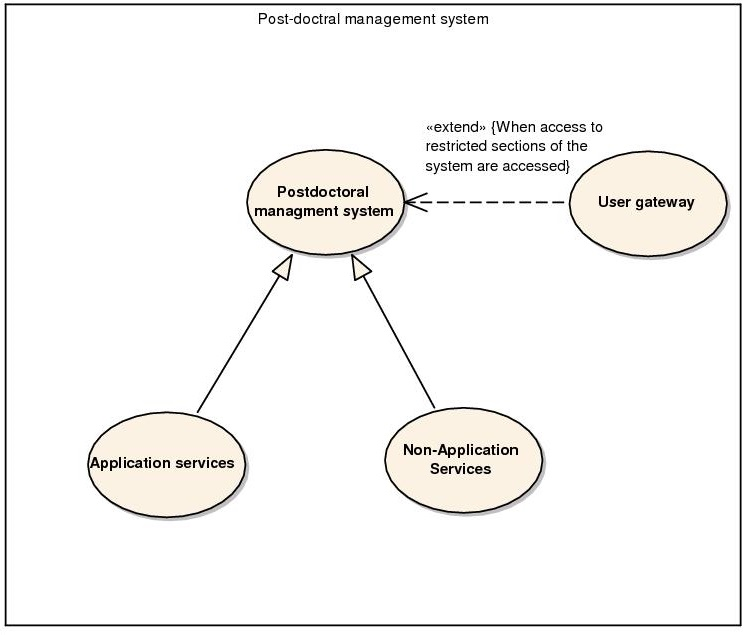
\includegraphics[scale=0.8]{../Images_Docs/Diagrams/Use case diagrams/Post-doctral fellowship management system1.jpg}}
\caption{Use case diagram of Post-doctoral application management system}
\end{figure}

\begin{figure}[H]
\centering	
\framebox{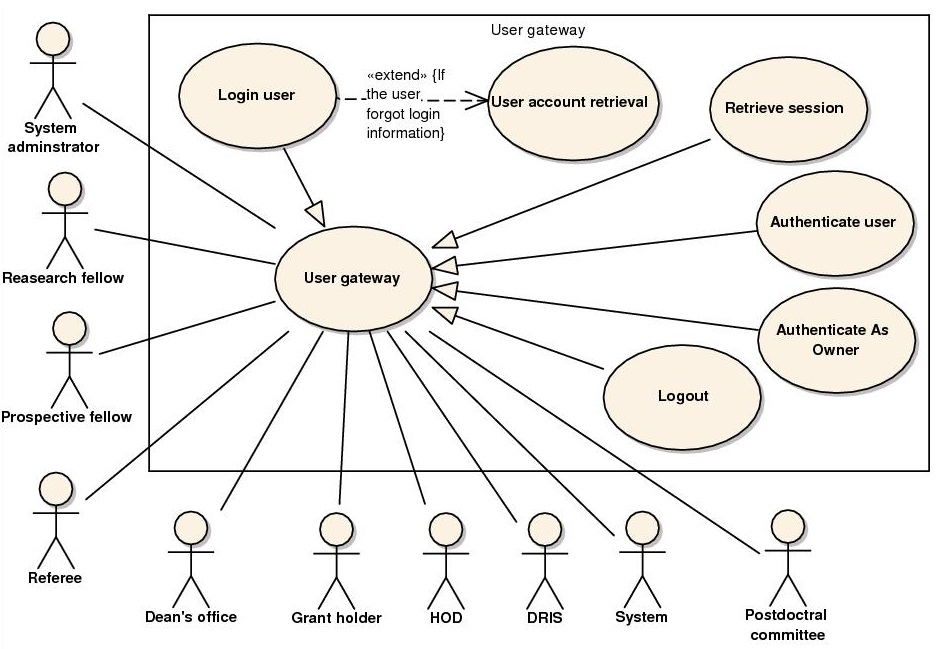
\includegraphics[scale=0.75]{../Images_Docs/Diagrams/Use case diagrams/User gateway1.jpg}}
\caption{Use case diagram of User gateway}
\end{figure}

\begin{figure}[H]
\centering	
\framebox{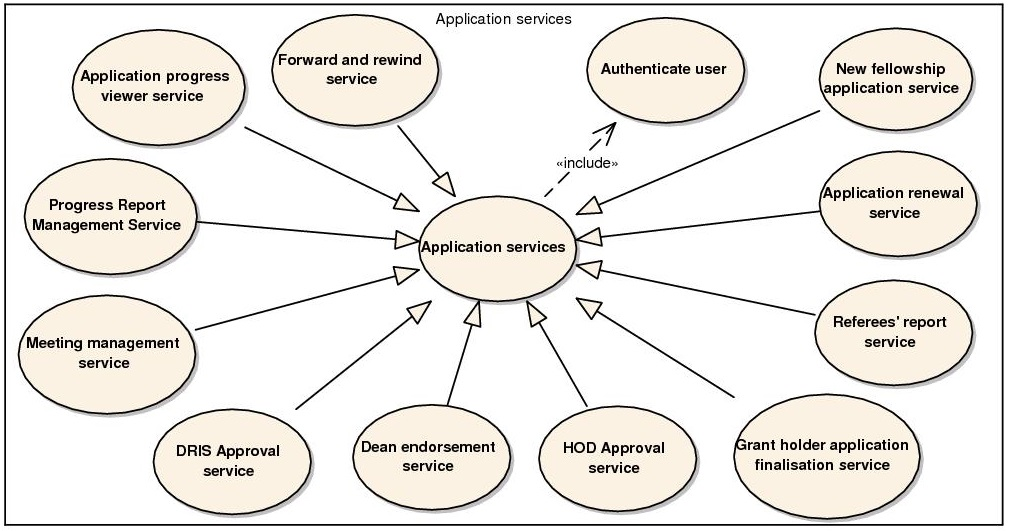
\includegraphics[scale=0.9]{../Images_Docs/Diagrams/Use case diagrams/Application services1.jpg}}
\caption{Use case diagram of Application services}
\end{figure}

\begin{figure}[H]
\centering	
\framebox{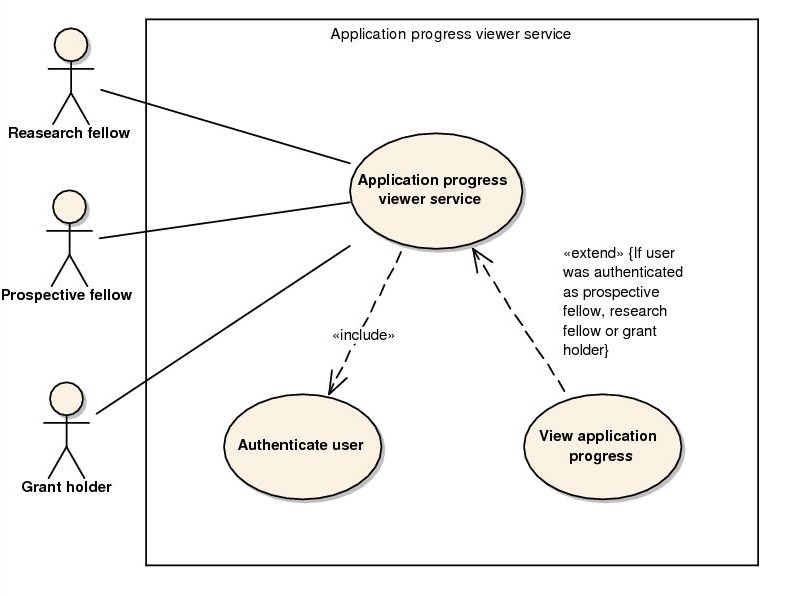
\includegraphics[scale=1]{../Images_Docs/Diagrams/Use case diagrams/Application progress viewer service1.jpg}}
\caption{Use case diagram of Application progress viewer service}
\end{figure}

\begin{figure}[H]
\centering	
\framebox{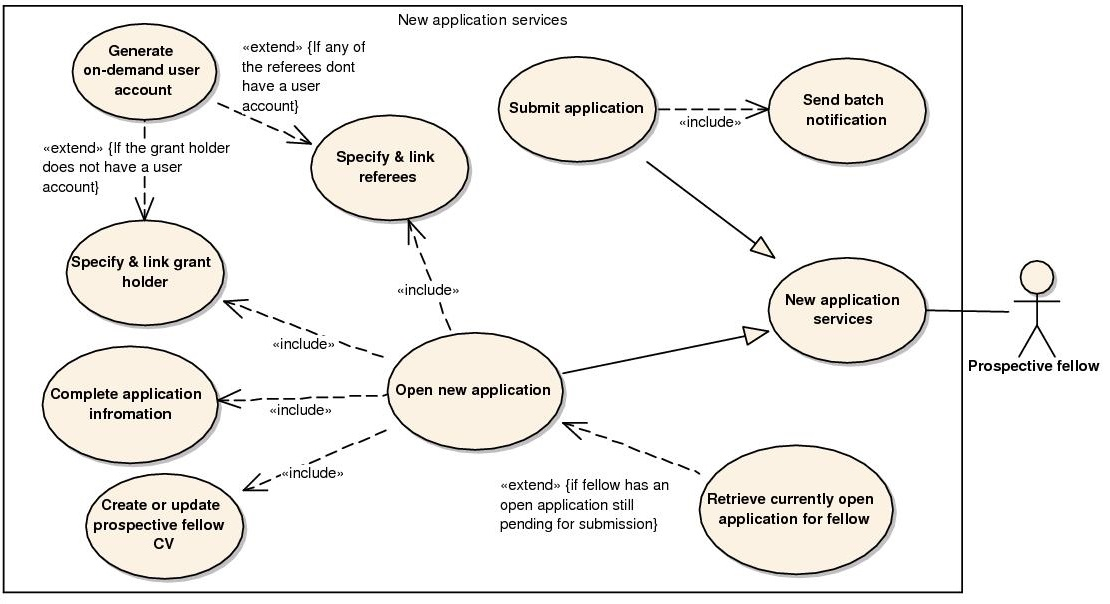
\includegraphics[scale=0.9]{../Images_Docs/Diagrams/Use case diagrams/New application service1.jpg}}
\caption{Use case diagram of New application services}
\end{figure}

\begin{figure}[H]
\centering	
\framebox{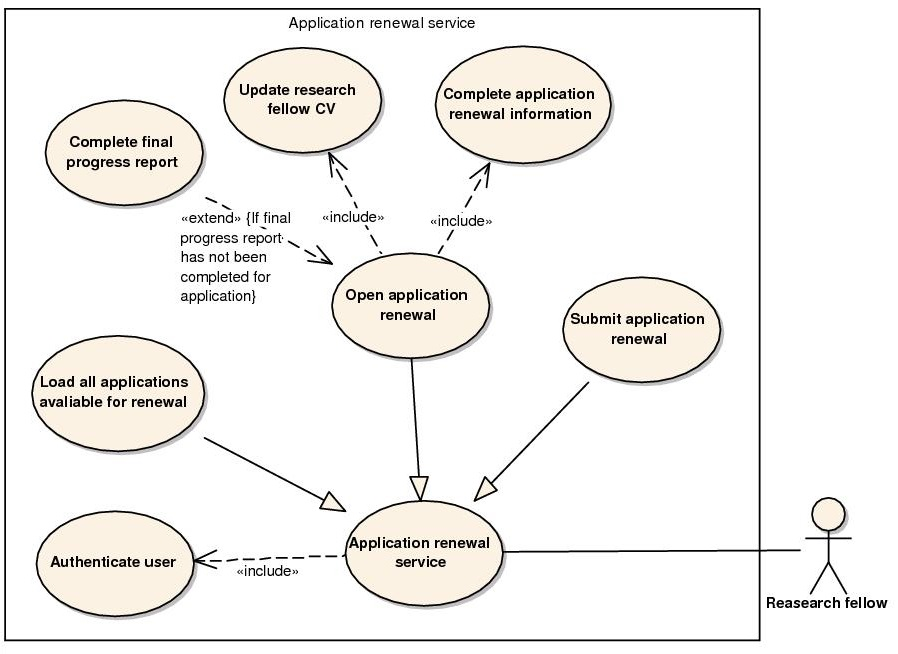
\includegraphics[scale=0.9]{../Images_Docs/Diagrams/Use case diagrams/Application renewal service1.jpg}}
\caption{Use case diagram of Application renewal service}
\end{figure}

\begin{figure}[H]
\centering	
\framebox{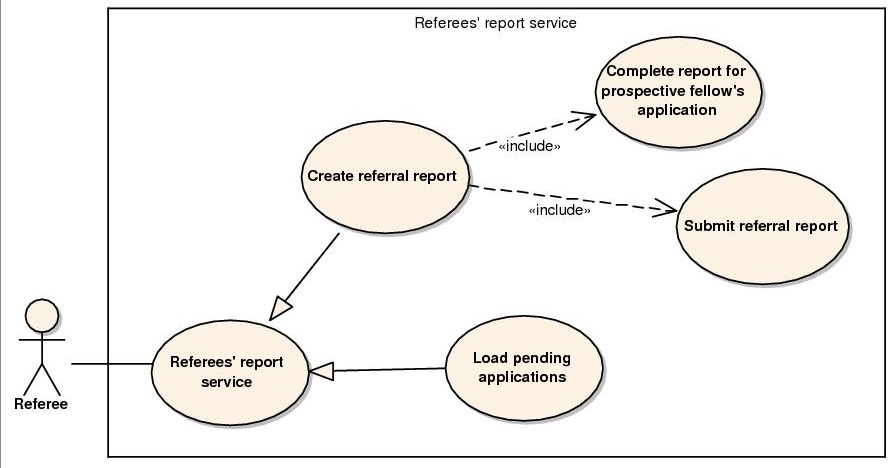
\includegraphics[scale=0.8]{../Images_Docs/Diagrams/Use case diagrams/Referees' report service1.jpg}}
\caption{Use case diagram of Referees' report service}
\end{figure}

\begin{figure}[H]
\centering	
\framebox{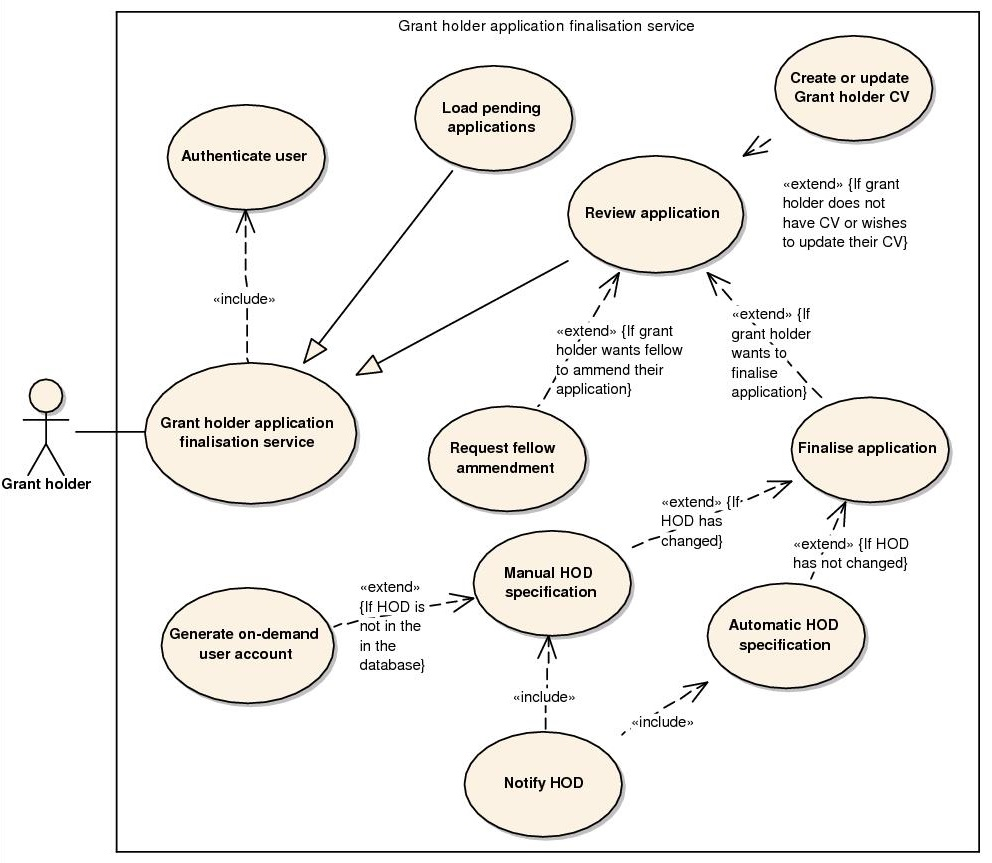
\includegraphics[scale=0.85]{../Images_Docs/Diagrams/Use case diagrams/Grant holder application finalisation service1.jpg}}
\caption{Use case diagram of Grant holder application finalisation service}
\end{figure}

\begin{figure}[H]
\centering	
\framebox{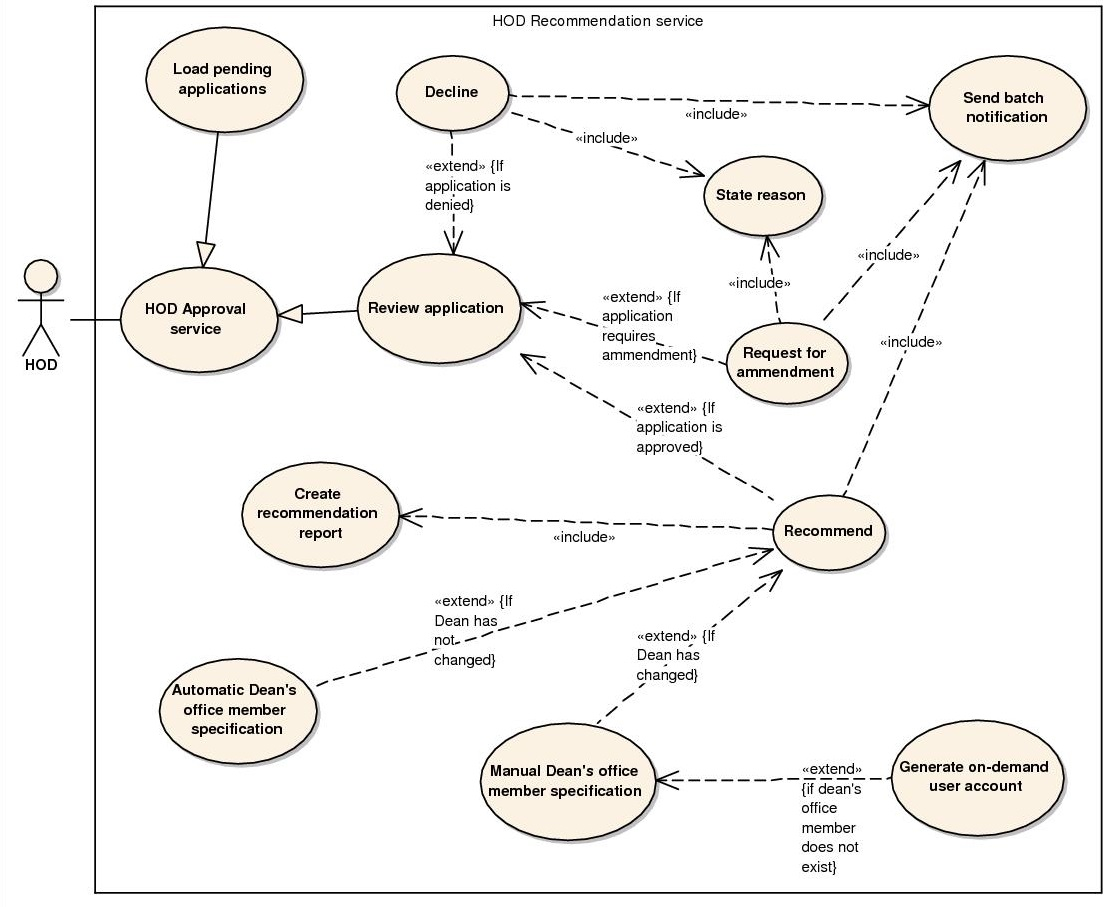
\includegraphics[scale=0.75]{../Images_Docs/Diagrams/Use case diagrams/HOD Recommendation service1.jpg}}
\caption{Use case diagram of HOD Recommendation service}
\end{figure}

\begin{figure}[H]
\centering	
\framebox{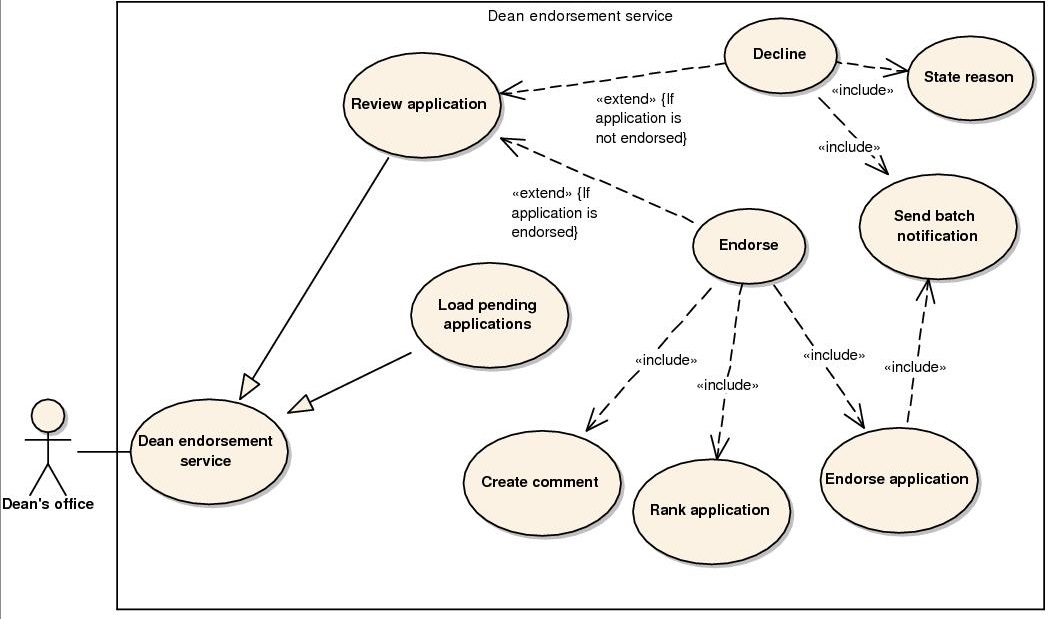
\includegraphics[scale=0.7]{../Images_Docs/Diagrams/Use case diagrams/Dean endorsement service1.jpg}}
\caption{Use case diagram of Dean endorsement service}
\end{figure}

\begin{figure}[H]
\centering	
\framebox{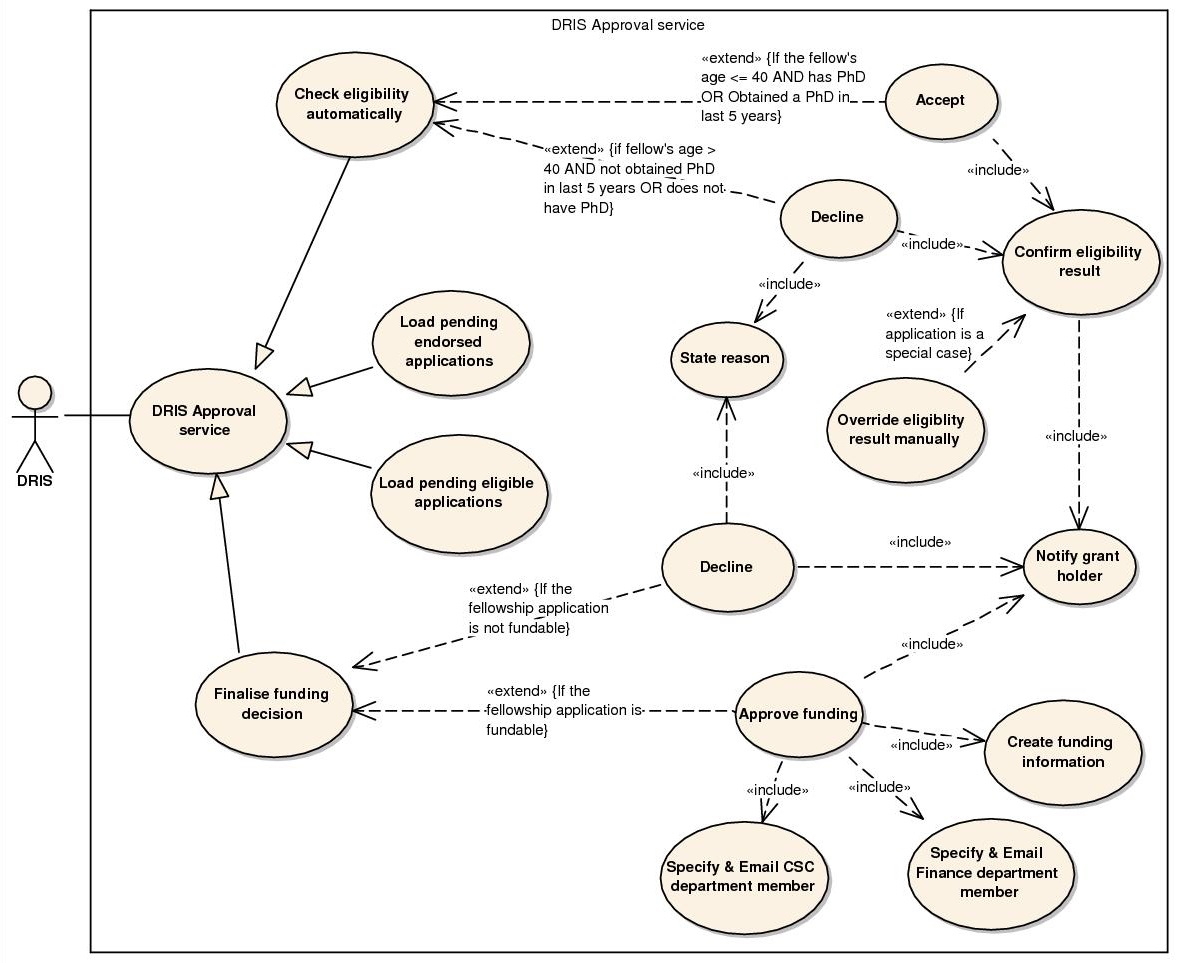
\includegraphics[scale=0.7]{../Images_Docs/Diagrams/Use case diagrams/DRIS approval service1.jpg}}
\caption{Use case diagram of DRIS approval service}
\end{figure}

\begin{figure}[H]
\centering	
\framebox{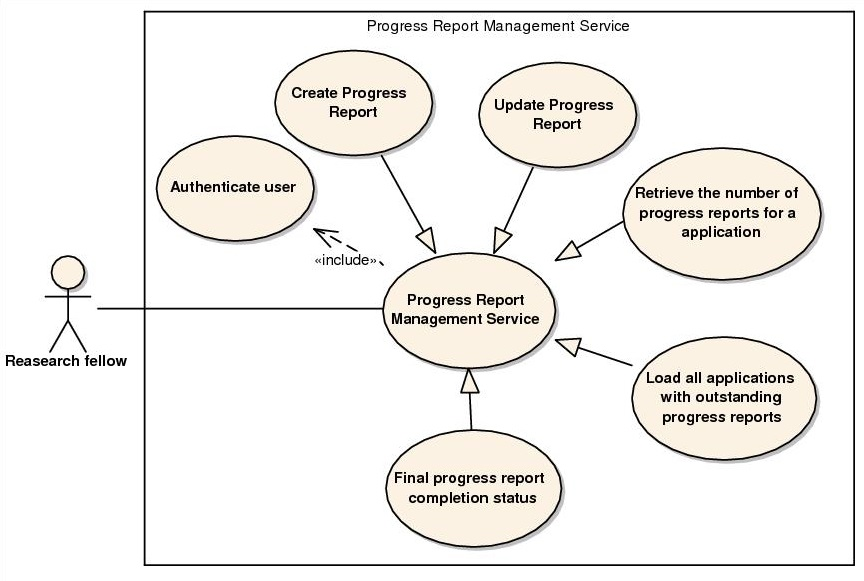
\includegraphics[scale=0.75]{../Images_Docs/Diagrams/Use case diagrams/Progress Report Management Service1.jpg}}
\caption{Use case diagram of Progress Report Management Service}
\end{figure}

\begin{figure}[H]
\centering	
\framebox{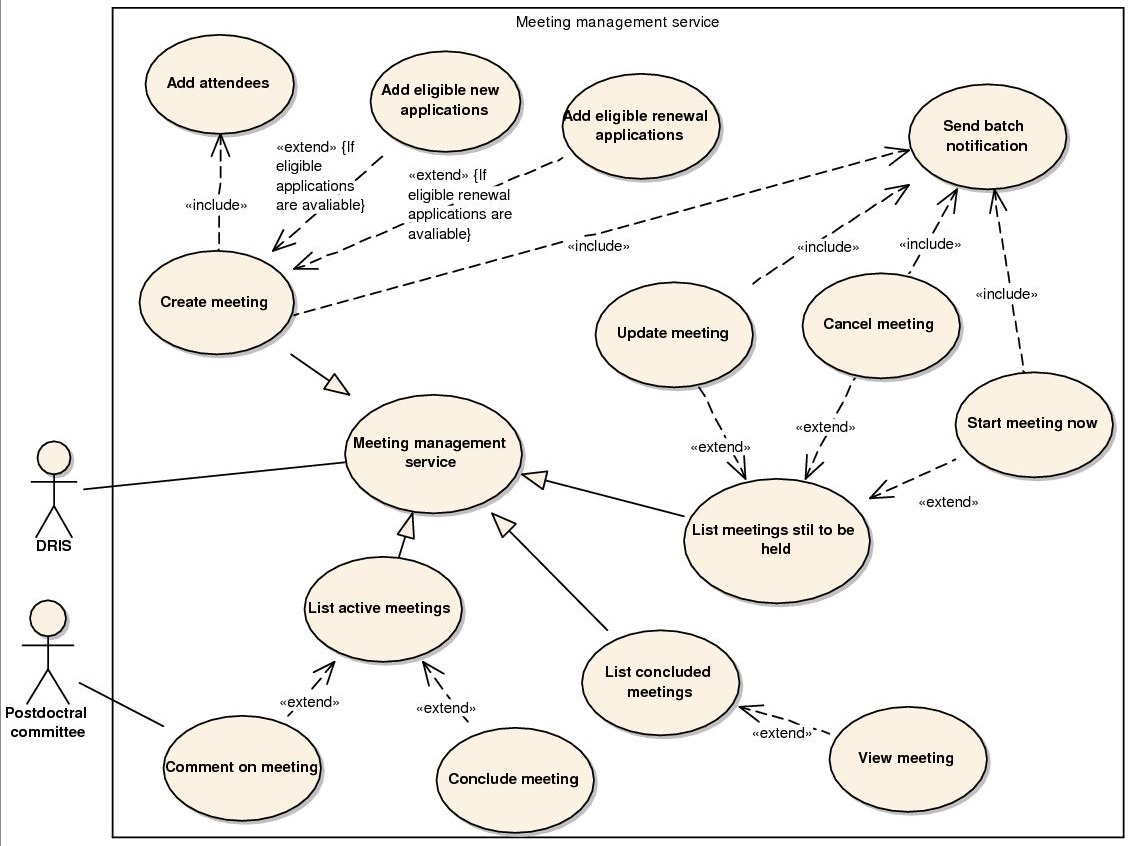
\includegraphics[scale=0.9]{../Images_Docs/Diagrams/Use case diagrams/Meeting management service1.jpg}}
\caption{Use case diagram of Meeting management service}
\end{figure}

\begin{figure}[H]
\centering	
\framebox{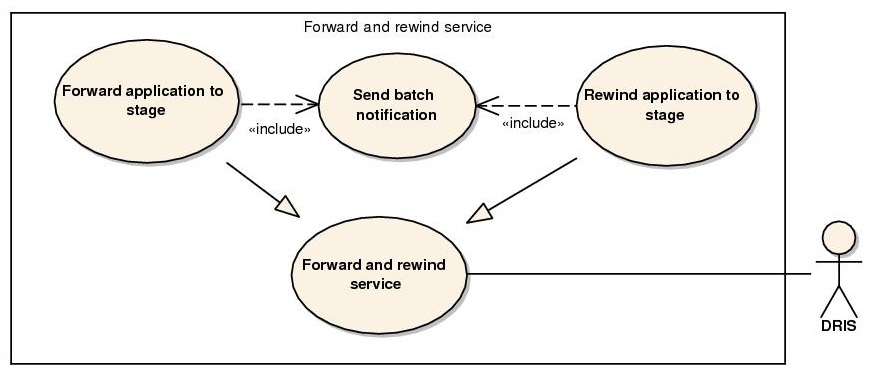
\includegraphics[scale=0.9]{../Images_Docs/Diagrams/Use case diagrams/Forward and Rewind Service1.jpg}}
\caption{Use case diagram of Forward and Rewind Service}
\end{figure}

\begin{figure}[H]
\centering	
\framebox{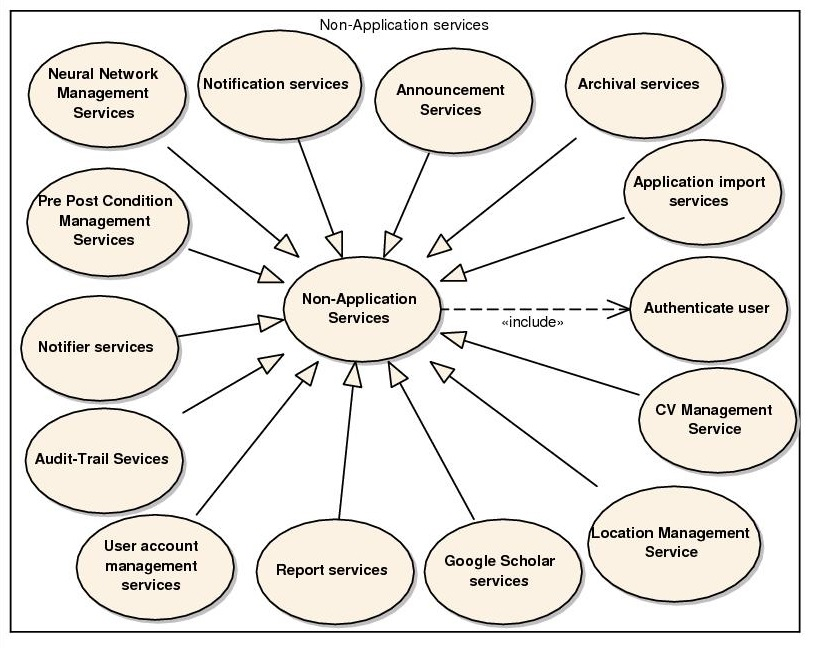
\includegraphics[scale=1]{../Images_Docs/Diagrams/Use case diagrams/Non-Application Services1.jpg}}
\caption{Use case diagram of Non-Application services}
\end{figure}

\begin{figure}[H]
\centering	
\framebox{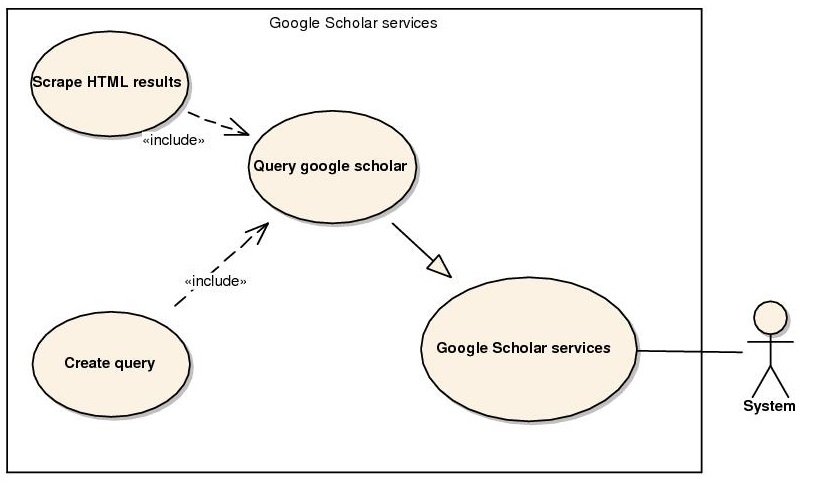
\includegraphics[scale=1]{../Images_Docs/Diagrams/Use case diagrams/Google Scholar services1.jpg}}
\caption{Use case diagram of Google Scholar services}
\end{figure}

\begin{figure}[H]
\centering	
\framebox{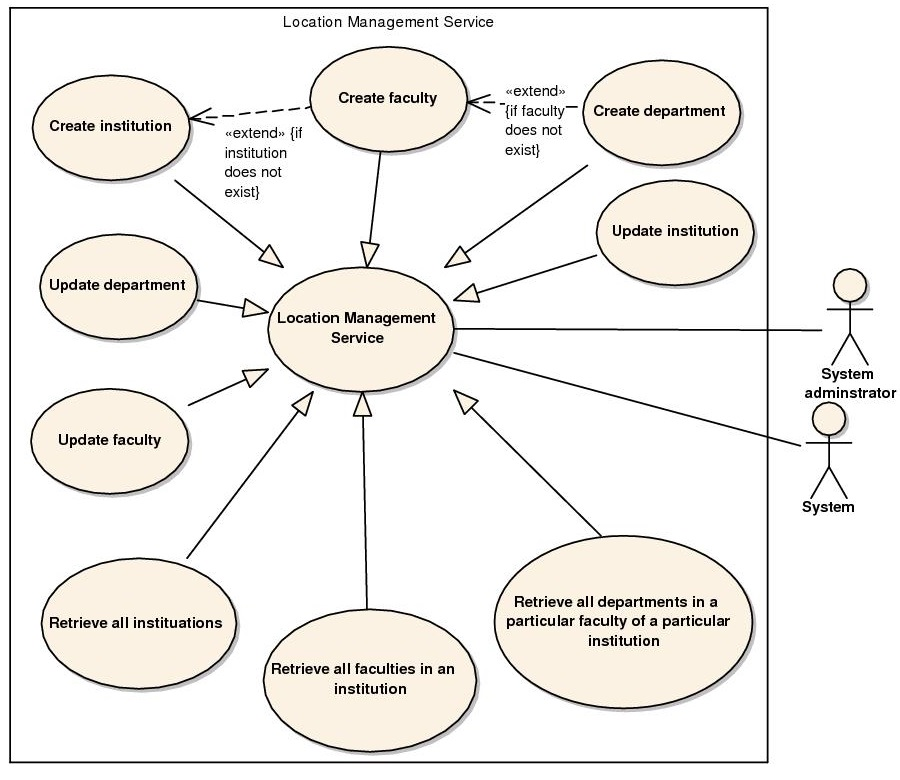
\includegraphics[scale=0.8]{../Images_Docs/Diagrams/Use case diagrams/Location Management Service1.jpg}}
\caption{Use case diagram of Location Management Service}
\end{figure}

\begin{figure}[H]
\centering	
\framebox{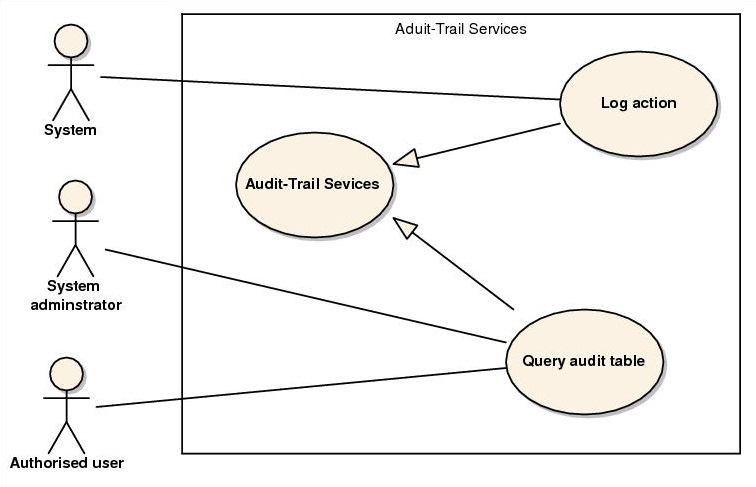
\includegraphics[scale=1]{../Images_Docs/Diagrams/Use case diagrams/Audit-Trail services1.jpg}}
\caption{Use case diagram of Audit-Trail services}
\end{figure}

\begin{figure}[H]
\centering	
\framebox{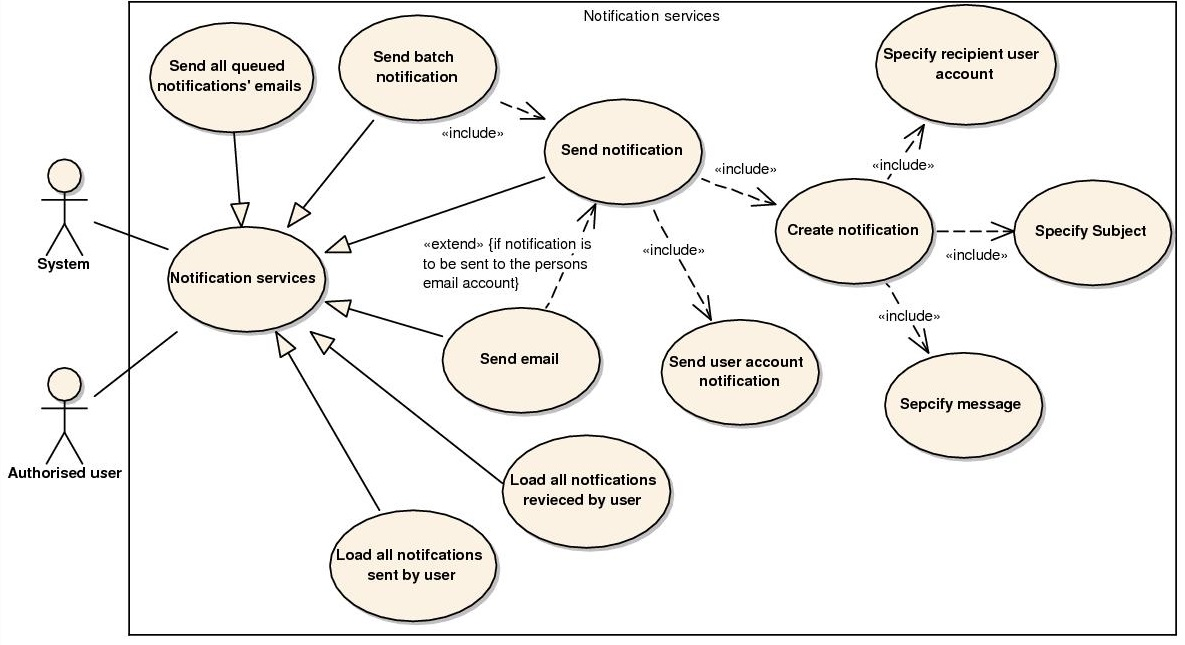
\includegraphics[scale=0.8]{../Images_Docs/Diagrams/Use case diagrams/Notification services1.jpg}}
\caption{Use case diagram of Notification services}
\end{figure}

\begin{figure}[H]
\centering	
\framebox{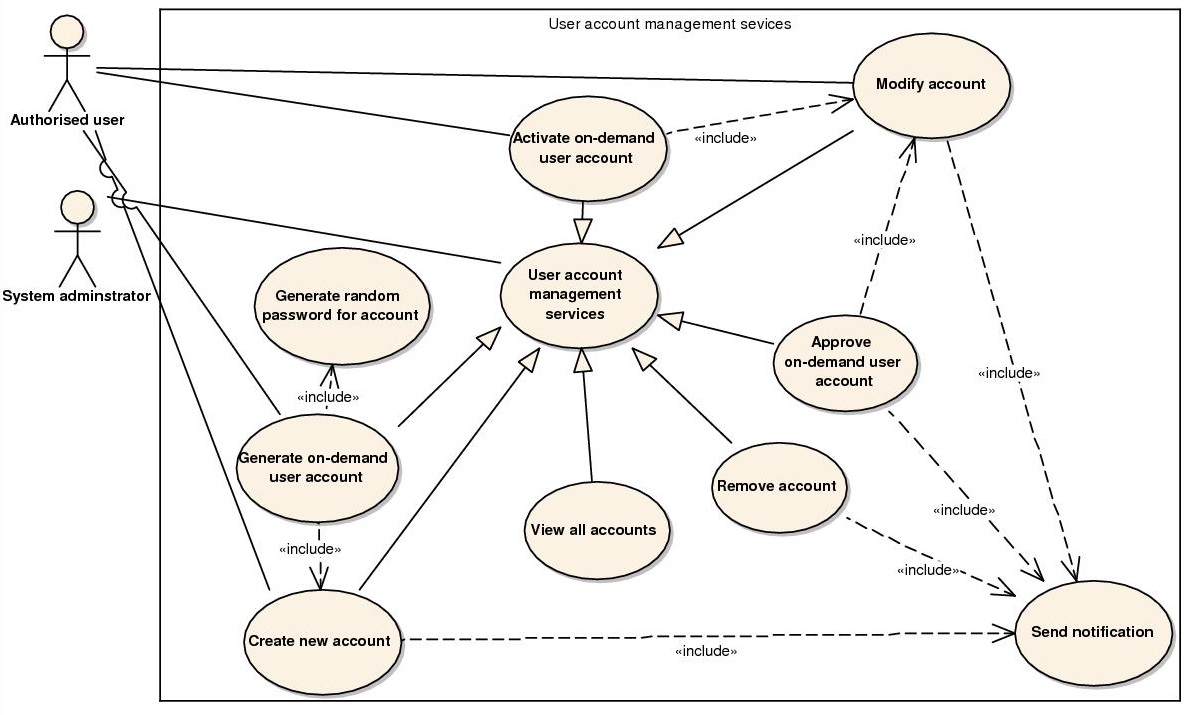
\includegraphics[scale=0.8]{../Images_Docs/Diagrams/Use case diagrams/User account management services1.jpg}}
\caption{Use case diagram of User account management services}
\end{figure}

\begin{figure}[H]
\centering	
\framebox{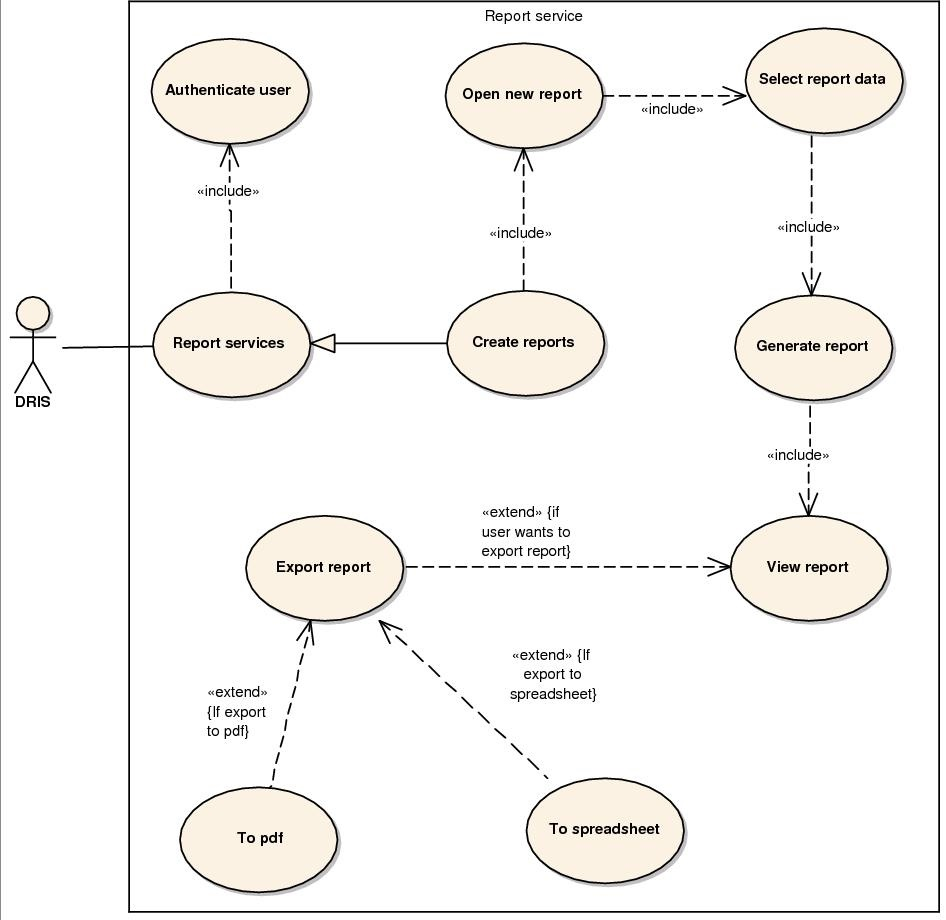
\includegraphics[scale=0.8]{../Images_Docs/Diagrams/Use case diagrams/Report services1.jpg}}
\caption{Use case diagram of Report service}
\end{figure}

\begin{figure}[H]
\centering	
\framebox{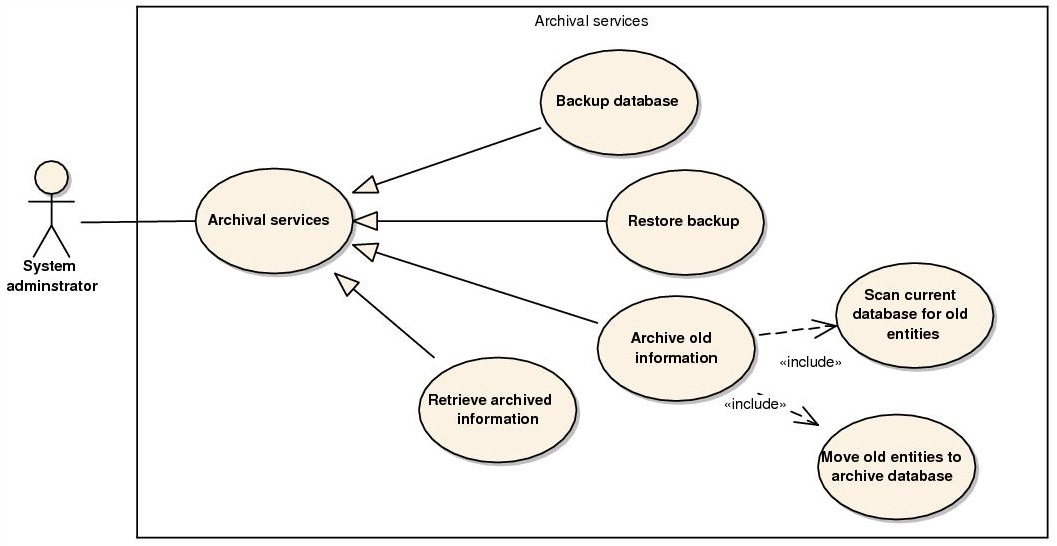
\includegraphics[scale=0.75]{../Images_Docs/Diagrams/Use case diagrams/Archival services1.jpg}}
\caption{Use case diagram of Archival services}
\end{figure}

\begin{figure}[H]
\centering	
\framebox{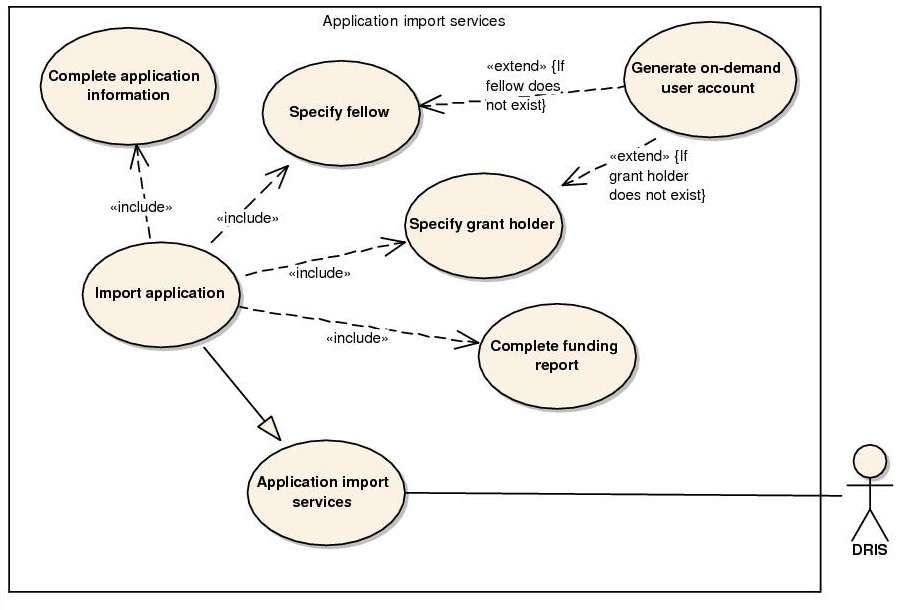
\includegraphics[scale=0.9]{../Images_Docs/Diagrams/Use case diagrams/Application import services1.jpg}}
\caption{Use case diagram of Application import services}
\end{figure}

\begin{figure}[H]
\centering	
\framebox{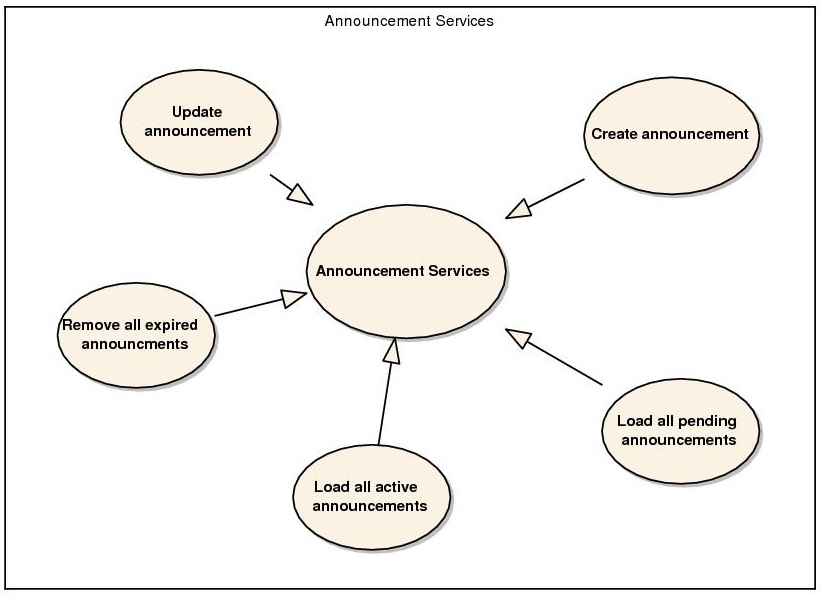
\includegraphics[scale=0.9]{../Images_Docs/Diagrams/Use case diagrams/Announcement Services1.jpg}}
\caption{Use case diagram of Announcement Services}
\end{figure}

\begin{figure}[H]
\centering	
\framebox{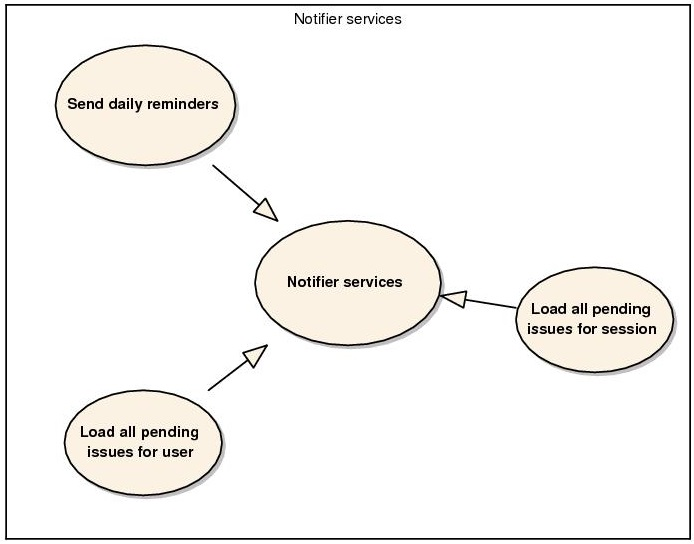
\includegraphics[scale=0.9]{../Images_Docs/Diagrams/Use case diagrams/Notifier services1.jpg}}
\caption{Use case diagram of Notifier services}
\end{figure}

\begin{figure}[H]
\centering	
\framebox{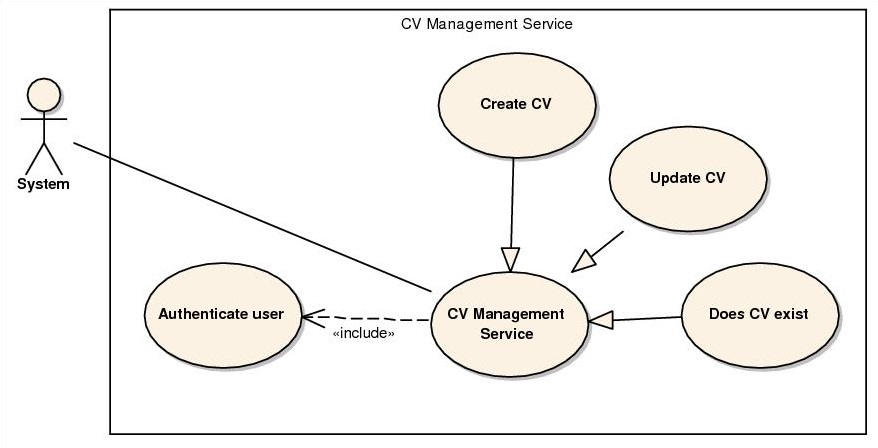
\includegraphics[scale=0.9]{../Images_Docs/Diagrams/Use case diagrams/CV Management Service1.jpg}}
\caption{Use case diagram of CV management service}
\end{figure}

\begin{figure}[H]
\centering	
\framebox{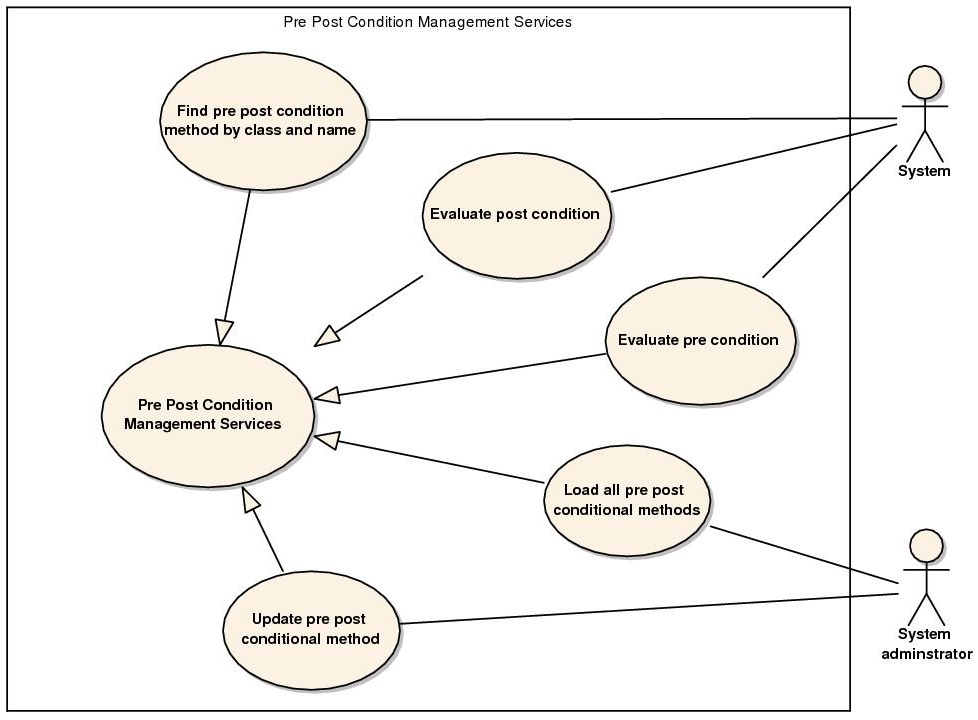
\includegraphics[scale=0.8]{../Images_Docs/Diagrams/Use case diagrams/Pre Post Condition Management Services1.jpg}}
\caption{Use case diagram of Pre post condition management services}
\end{figure}

\begin{figure}[H]
\centering	
\framebox{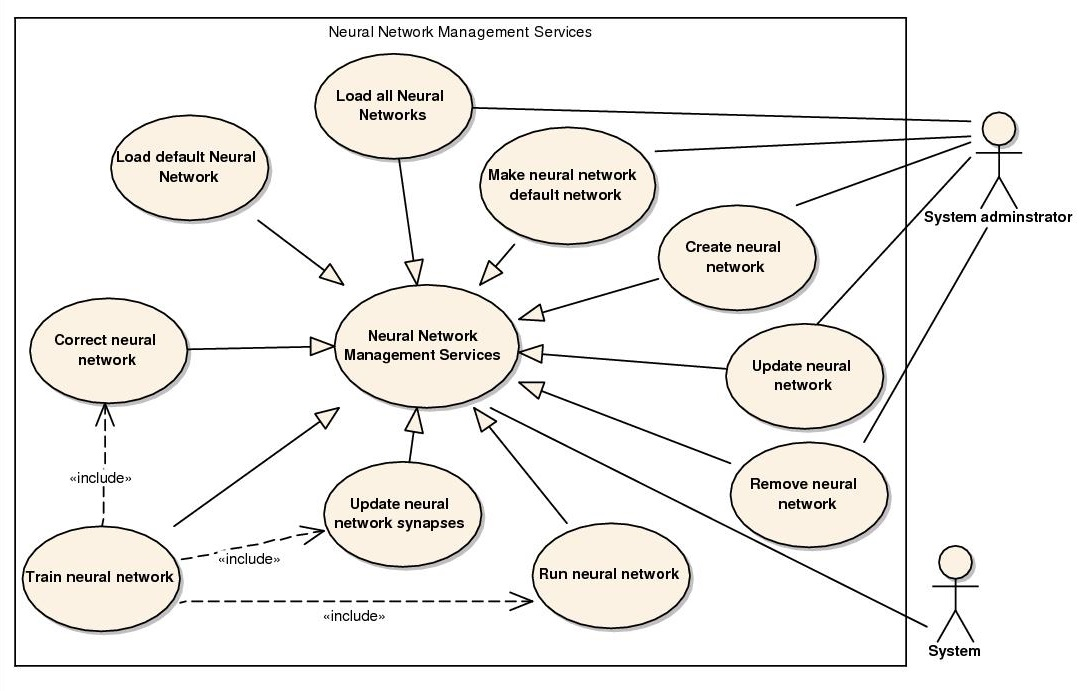
\includegraphics[scale=0.8]{../Images_Docs/Diagrams/Use case diagrams/Neural Network Management Services1.jpg}}
\caption{Use case diagram of Neural Network Management Services}
\end{figure}

\begin{figure}[H]
\centering	
\framebox{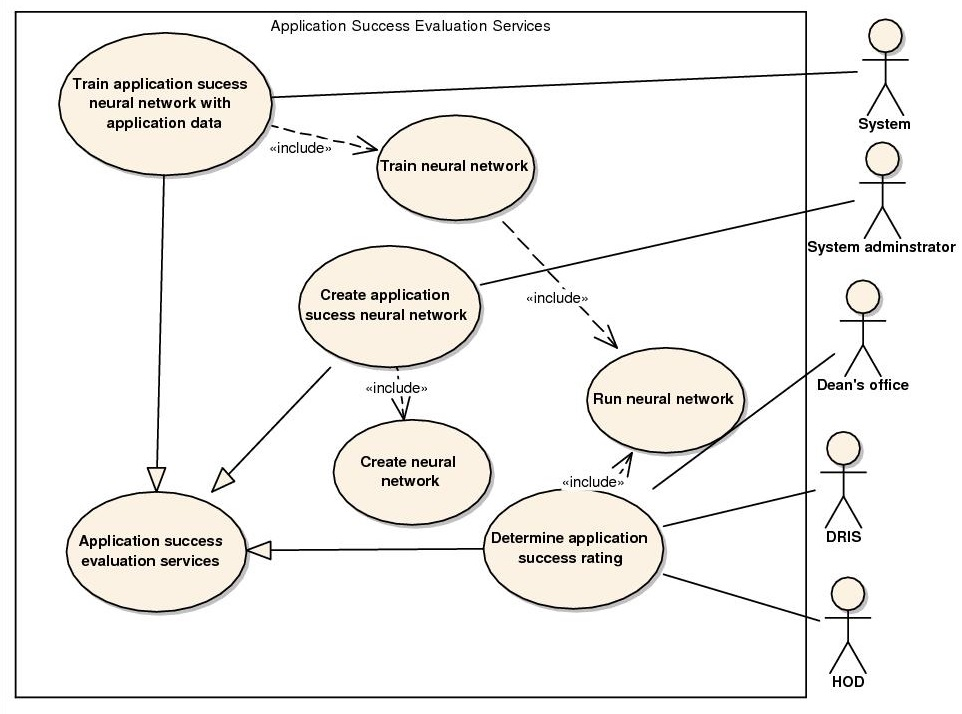
\includegraphics[scale=1]{../Images_Docs/Diagrams/Use case diagrams/Application Success Evaluation Services1.jpg}}
\caption{Use case diagram of Application success evaluation services}
\end{figure}



\newpage
\subsection{Use case prioritization}
\vspace{0.2in}
This section states the ranking in terms of priority of the service use case per use case diagram figure. The priorities are: Critical, Important and Nice to have.\\ 

\subsubsection{User gateway}
\begin{itemize}
	\item Login user: Critical	
	\item Create prospective fellow user account: Critical
	\item Generate on-demand user account: Critical
	\item Activate on-demand user account: Critical
	\item Authenticate user: Critical
	\item User account retrieval: Important
\end{itemize}
\subsubsection{Application services}
\begin{itemize}
	\item New application service: Critical
	\item Application renewal service: Critical
	\item Referees' report service: Critical
	\item Grant holder application finalisation service: Critical
	\item HOD Approval service: Critical
	\item Dean endorsement service: Critical
	\item DRIS approval service: Critical
	\item Progress report management service: Critical		
	\item Meeting management service: Important
	\item Application progress viewer service: Important
	\item Fast-forward and rewind service: Important
	\item Application success evaluation service: Nice to have 		
\end{itemize}

\subsubsection{Non-Application services}
\begin{itemize}
	\item Notification services: Critical
	\item User account management services: Critical
	\item Audit-Trail services: Critical
	\item CV management service: Critical
	\item Location management service: Critical
	\item Report services: Important
	\item Notifier services: Important
	\item Archival services: Nice to have
	\item Application import services: Nice to have
	\item Google scholar services: Nice to have
	\item Announcement services: Nice to have
	\item Neural network management services: Nice to have
	\item Pre post condition management services: Nice to have								
\end{itemize}



\vspace{0.2in}
\newpage
\subsection{Services contracts for use cases} %Mathys
\vspace{0.2in}

This section states the preconditions and postconditions of the each use case per use case diagram figure. \\

\subsubsection{Preconditions}
These are conditions that must be met by the system or user before they are allowed to use the use case.\\
\begin{itemize}
	\item \textbf{User gateway}
		\begin{itemize}
			\item Login user: Requesting user is a user of the system and not logged in.
			\item User account retrieval: Requesting user has forgotten their user credentials.				
			\item Authenticate user: User is logged in.	
			\item Authenticate as owner: User is logged in and an object has been selected for ownership testing.
			\item Logout: The user is logged in.
			\item Retrieve session: The user is logged in.						
		\end{itemize}
		
	\item\textbf{Application services}
		\begin{itemize}
			\item New application services: The user is a prospective fellow.
			\item Application renewal service: Renewals are open and the user is a research fellow that is still in possession of active fellowship.
			\item Referees' report service: If user is a referee.
			\item Grant holder application finalisation service:  The user is a grant holder.
			\item HOD Approval service: The user is a HOD.
			\item Dean endorsement service: The user is a member of the dean's office.
			\item DRIS Approval service:  The user is a member of the DRIS.
			\item Meeting management service:  The user is a member of the DRIS or post-doctoral committee.
			\item Application progress viewer service: The user is a prospective fellow or research fellow or grant holder or DRIS member.
			\item Forward and rewind service: The user is a member of the DRIS.
			\item Progress report management service: The user is a research fellow or a member of the DRIS.	
		\end{itemize}
		
	\item \textbf{Application progress viewer service}
		\begin{itemize}
			\item View application progress: A application is selected.
			\item View application stage attachments: A application is selected.
		\end{itemize}
		
	\item \textbf{New application services}
		\begin{itemize}
			\item Generate on-demand user account: The prospective fellow has identified a referee or grant holder not on the system.
			\item Submit information: The fellow's cv, application information, grant holder and referee information is complete.
			\item Open new application: An application is currently open for the fellow or all applications owned by the fellow are completed/closed/terminated.			
		\end{itemize}
	
	\item \textbf{Application renewal service}
		\begin{itemize}
			\item Load all applications available for renewal: There are applications of the research fellow that are available for renewal.
			\item Open renewal application: The research fellow has a fellowship that is renewable or has a currently open renewal application.
			\item Complete progress report: The final progress report has not been completed.				
			\item Submit renewal application: If all the required information for the renewal has been completed.									
		\end{itemize}
	
	\item \textbf{Referees' report service}
		\begin{itemize}
			\item Load pending applications: There are submitted applications that need a referral report form the referee.
			\item Create referral report: The application selected needs a referral report from the referee.				
			\item Submit referral report: If the referral report has been completed.									
		\end{itemize}
		
	\item \textbf{Grant holder application finalisation service}
		\begin{itemize}
			\item Load pending applications: There are referred applications that need to be finalised by the grant holder.
			\item Create or Update Grant holder CV: The grant holder does not have a CV or has a CV.
			\item Review application: There are pending applications.
			\item Finalise application: The grant holder has selected an application that is pending. 
			\item Request fellow amendment: The grant holder has selected an application that is pending.
			\item Decline application: The grant holder has selected an application that is pending.
			\item Generate on-demand user account: The grant holder has identified a HOD not on the system.								
		\end{itemize}
			
	\item \textbf{HOD Recommendation service}
		\begin{itemize}
			\item Load pending applications: There are finalised applications that need to be recommended by the HOD.
			\item Review application: There are pending applications.
			\item Recommend: The HOD has selected an application that is pending. 
			\item Decline: The HOD has selected an application that is pending. 
			\item Request for amendment: The HOD has selected an application that is pending. 
			\item Create recommendation report: The selected application has been marked for recommendation.				
			\item Generate on-demand user account: The grant holder has identified a Dean's office member not on the system.										
		\end{itemize}
		
	\item \textbf{Dean endorsement service}
		\begin{itemize}
			\item Load pending applications: There are recommend applications that need to be endorsed by the Dean's office.
			\item Review application: There are pending applications.
			\item Endorse: The Dean's office member has selected an application that is pending.  
			\item Decline: The Dean's office member has selected an application that is pending.										
		\end{itemize}
	
	\item \textbf{DRIS approval service}
		\begin{itemize}
			\item Load pending endorsed applications: There are endorsed applications that need to be checked for eligibility by the DRIS.
			\item Load pending eligible applications: There are eligible applications that need to be approved for funding by the DRIS.
			\item Check eligibility automatically: There are endorsed application available for  eligibility check.
			\item Decline eligibility: The fellow is older than 40 and has not obtained their PhD in the last 5 years or if the prospective fellow does not have a PhD.
			\item Accept: The fellow is younger than 40 or is 40 and they have a PhD or if they have obtained a PhD in the last 5 years.
			\item Override eligibility result manually: Application is a special case.
			\item Confirm eligibility result: A eligibility result for the selected application is determined. 
			\item Finalise funding decision: There are eligible applications available for  funding approval.			
			\item Approve funding: The Dean's office member has selected an application that has a pending funding decision.	
			\item Decline funding: The Dean's office member has selected an application that has a pending funding decision.
			\item Fund application: All funding information is complete.											
		\end{itemize}
	
	\item \textbf{Progress report management service}
		\begin{itemize}
			\item Create progress report: The research fellow has an outstanding progress report.
			\item Update progress report: A valid progress report has been selected.
			\item Retrieve the number of progress reports for a application: A valid application has been selected.
			\item Load all applications with outstanding progress reports: There are applications with outstanding progress reports.
			\item Final progress report completion status: A valid application has been selected.						
		\end{itemize}

	\item \textbf{Meeting management service}
		\begin{itemize}			
			\item Create meeting: The user is a DRIS member.
			\item Add eligible new applications: There are eligible new applications available.
			\item Add eligible renewal applications: There are eligible renewal applications available.
			\item Add attendees: There are post doctoral committee members available.
			\item List meetings still to be held: There are meetings still to be held available.
			\item Update meeting: The meeting is not active nor concluded and the user is a DRIS member.
			\item Cancel meeting: The meeting is not active nor concluded and the user is a DRIS member.
			\item Start meeting: The meeting is not active nor concluded and the user is a DRIS member.
			\item List active meetings: There are active meetings available.
			\item Comment on meeting: The selected meeting is active and the user is a attendee.
			\item Conclude meeting: The selected meeting is active and the user is a DRIS member.	
			\item List concluded meetings: There are meetings that have been concluded available.						
		\end{itemize}

	\item \textbf{Forward and rewind service}
		\begin{itemize}
			\item Forward application to stage: The selected application has a status between Open and recommended.
			\item Rewind application to stage: The selected application has a status between Submitted and Declined.						
		\end{itemize}

	\item \textbf{Non-Application services}
		\begin{itemize}
			\item Notification services: The user is the system or authorised user.
			\item User account management services: The user is the system or system administrator or owner of an account.
			\item Archival services: The user is a system administrator.
			\item CV Management service: The user has a CV or needs to create a CV.
			\item Location management service: The user is the system administrator or the system.
			\item Google scholar services: The user is the system.
			\item Report services: The user is a DRIS member or system administrator.
			\item Announcement services: The user is a DRIS member or system administrator.
			\item Audit-Trail service: The user is a system administrator or the system.
			\item Notifier service: The user is the system.						
		\end{itemize}
		
	\item \textbf{Google scholar services}
		\begin{itemize}
			\item Query Google scholar: Google scholar is available and the query is valid.							
		\end{itemize}
		
	\item \textbf{Location management services}
		\begin{itemize}
			\item Create Faculty: The institution exists.
			\item Create Department: The faculty under which it falls exist.
			\item Update Institution: A valid institution is selected.
			\item Update Faculty: A valid faculty is selected. 	
			\item Update Department: A valid department is selected. 
			\item Retrieve all Institutions: There are institutions available.
			\item Retrieve all faculties in an institution: There are faculties available under the institution.
			\item Retrieve all departments in a particular faculty of a particular institution: There are departments available under the faculty.	 						
		\end{itemize}
	
	\item \textbf{Audit-Trail services}
		\begin{itemize}
			\item Log action: If requesting user is the system and a User has preformed a critical task.
			\item Query audit table: If the user is system administrator.										
		\end{itemize}
	
	\item \textbf{Notification services}
		\begin{itemize}
			\item Send all queued notifications' emails: There are unsent emails available and 1 minute has passed since the last check.
			\item Create notification: The message has a recipient and message.				
			\item Send user account notification: If notification is ready to be sent.
			\item Send email: If notification is ready to be sent or a standalone email is to be sent.
			\item Send batch notifications: There is more then one notification request waiting.
			\item Load all notifications received by user: There are notifications that the user has received available.
			\item Load all notifications sent by user: There are notifications that the user has sent available.	
		\end{itemize}
	
	\item \textbf{User account management services}
		\begin{itemize}
			\item Create new account: The user is a system administrator or is a prospective fellow.
			\item Modify account: The user is a system administrator or is the owner of the account.				
			\item Remove account: The user is a system administrator.	
			\item View all accounts: The user is a system administrator.
			\item Generate on-demand user account: The system requires a new account to be created for a person not the system.
			\item Approve on-demand user account: The user is a system administrator and there are pending on-demand user accounts available.
			\item Activate on-demand user account: The user is the owner of the account and the account is a dormant user account.				
		\end{itemize}
	
	\item \textbf{Report service}
		\begin{itemize}
			\item Create report: The user is a system administrator or a DRIS member.
			\item Open new report: No report is currently open.
			\item Select report data: A report is open and there is data available for report.
			\item Generate report: Data has been selected for the report.
			\item View report: The report has been generated.
			\item Export report: The user wants to export report and the user is busy viewing the report.
			\item To Spreadsheet: The user wants to export report to a MS Excel spreadsheet file.
			\item To pdf: The user wants to export report to a PDF.	
		\end{itemize}
	
	
	\item \textbf{Archival services}
		\begin{itemize}
			\item Retrieve archived information: The user is a system administrator or the system and there is any archived information available.
			\item Archive old information: The user is a system administrator or the system.	
			\item Backup database: The user is a system administrator or the system.	
			\item Restore backup: The user is a system administrator or the system and there are backups available.			
		\end{itemize}
		
	\item \textbf{Application import services}
		\begin{itemize}
			\item Import application: The user wants to create a already funded and still active application that already exists but not on the system.
			\item Generate on-demand user account: If the fellow or grant holder of the application does not exist. 					
		\end{itemize}
		
	\item \textbf{Announcement services}
		\begin{itemize}
			\item Create announcement: The user wants to create a new announcement.
			\item Update announcement: The user wants to update the selected pending/active announcement.
			\item Remove all expired announcements: There are expired announcements on the system and a 1 Day has passed since the last check.
			\item Load all active announcements: There are active announcements available.
			\item Load all pending announcements: There are pending announcements available. 				
		\end{itemize}
		
	\item \textbf{Notifier services}
		\begin{itemize}
			\item Send daily reminders: There are issues outstanding for any user and a day has passed since the last check.
			\item Load all pending issues for user: A valid user is selected and the user is the system and there are outstanding issues for the user.	
			\item Load all pending issues for session: The user is the owner of the session and there are outstanding issues for the user.				
		\end{itemize}
		
	\item \textbf{CV management services}
		\begin{itemize}
			\item Create CV: The system requires to create a CV for some user.
			\item Update CV: The system requires to update a CV for an existing CV of a particular user who is the owner of the CV.					
		\end{itemize}
	\item \textbf{Pre post condition management services}
			\begin{itemize}
				\item Find pre post condition method by class and name: Method must exist.
				\item Evaluate post condition: Post condition script must exist.
				\item Evaluate pre condition: Pre condition script must exist.
				\item Update pre post conditional method: A valid method must be selected.	
				\item Load all pre post conditional methods: There must be at least 1 pre post conditional method available. 			
			\end{itemize}
	\item \textbf{Neural network management services}
			\begin{itemize}
				\item Load all neural networks: There must be at least 1 neural network available.
				\item Make neural network default network: A valid neural network must be selected.
				\item Create a neural network: The system wants to create a neural network.
				\item Update a neural network: A valid neural network has been selected.
				\item Remove a neural network: A valid neural network has been selected.			
			\end{itemize}
	\item \textbf{CV management services}
			\begin{itemize}
				\item Create CV: The system requires to create a CV for some user.
				\item Update CV: The system requires to update a CV for an existing CV of a particular user who is the owner of the CV.					
			\end{itemize}	
\end{itemize}	

\subsubsection{Postconditions}
These are conditions that must be met by the system and the data after the use case has been used.\\
\begin{itemize}
	\item \textbf{User gateway}
		\begin{itemize}
			\item Login user: The user is logged in and has a session.
			\item User account retrieval: The password has been reset and the user is notified.				
			\item Authenticate user: The user is authenticated with the required security role or has not been authenticated.	
			\item Authenticate as owner: The user is the owner of the object or is not the owner.
			\item Logout: The user is logged out and has its session invalidated.
			\item Retrieve session: The user's session is retrieved.						
		\end{itemize}
		
	\item\textbf{Application services}
		\begin{itemize}
			\item New application services: The user can make use of these services.
			\item Application renewal service: The user can make use of these services.
			\item Referees' report service: The user can make use of these services.
			\item Grant holder application finalisation service:  The user can make use of these services.
			\item HOD Approval service: The user can make use of these services.
			\item Dean endorsement service: The user can make use of these services.
			\item DRIS Approval service:  The user can make use of these services.
			\item Meeting management service:  The user can make use of these services.
			\item Application progress viewer service: The user can make use of these services.
			\item Forward and rewind service: The user can make use of these services.
			\item Progress report management service: The user can make use of these services.	
		\end{itemize}
		
	\item \textbf{Application progress viewer service}
		\begin{itemize}
			\item View application progress: The various stages completed thus far by the application is available for viewing.
			\item View application stage attachments: The various stage attachments made thus far to the application is available for viewing.
		\end{itemize}
		
	\item \textbf{New application services}
		\begin{itemize}
			\item Open new application: The current open application is opened for editing or a new open application has been created.
			\item Generate on-demand user account: The identified referees or grant holder has been added to the system and has a pending user account.
			\item Create or update prospective fellow CV: The prospective fellow's CV has been created or updated.
			\item Complete application information: The application's information is stored.
			\item Specify and link grant holder: Grant holder has been linked to the application.
			\item Specify and link referees: All the referees have been linked to the application.
			\item Submit information: The application status is changed to submitted if it has referees or referred if it has none or is a renewal.
			\item Send batch notifications: The fellow and the next stage's members are notified, either referees or grant holder. 		
		\end{itemize}
	
	\item \textbf{Application renewal service}
		\begin{itemize}
			\item Load all applications available for renewal: All applications available for renewal has been loaded.
			\item Open renewal application: The currently open renewal application is opened for editing or a new renewal is created for the selected application.
			\item Complete progress report: The final progress report is stored.
			\item Update research fellow CV: The research fellow's CV is updated.
			\item Complete application renewal information: The renewal application information is stored.				
			\item Submit renewal application: The application status is changed to referred.
			\item Send batch notifications: The fellow and the grant holder are notified.									
		\end{itemize}
	
	\item \textbf{Referees' report service}
		\begin{itemize}
			\item Load pending applications: All submitted applications with pending reports are loaded.
			\item Create referral report: The referral report is generated.				
			\item Submit referral report: If the referral report is attached to the application. If it is the last referral report for the application the application status is changed to Referred.
			\item Send batch notifications: The fellow and the grant holder are notified.									
		\end{itemize}
		
	\item \textbf{Grant holder application finalisation service}
		\begin{itemize}
			\item Load pending applications: All the referred applications that need to be finalised by the grant holder are loaded.
			\item Create or Update Grant holder CV: The grant holders CV is stored.
			\item Review application: A pending application has been selected and is visible.
			\item Finalise application: The application status is changed to Finalised.
			\item Request fellow amendment: The application is changed to an Open application.
			\item Decline: The application status is changed to declined and the reason is stored.
			\item Automatic HOD specification: A HOD has been selected for sending the application to.
			\item Manual HOD specification: A HOD has been selected for sending the application to.
			\item Generate on-demand user account: Identified a HOD has been created a pending account on the system.
			\item Send batch notifications: The fellow, the grant holder and if finalised the specified HOD are notified.								
		\end{itemize}
			
	\item \textbf{HOD Recommendation service}
		\begin{itemize}
			\item Load pending applications: All the finalised applications that need to be recommended by the HOD are loaded.
			\item Review application: A pending application has been selected and is visible.
			\item Recommend: The applications status is changed to recommend and forwarded to the next stage.
			\item Decline: The application status is changed to declined and the reason is stored.
			\item Request for amendment: The application status has changed to finalised. 
			\item Create recommendation report: A recommendation report is created for the application.				
			\item Automatic Dean's offiece member specification: A member of the dean's office has been selected for sending the application to.
			\item Manual Dean's offiece member specification: A member of the dean's office has been selected for sending the application to.
			\item Generate on-demand user account: The grant holder has identified a Dean's office member not on the system.			
			\item Send batch notifications: The fellow, the grant holder and if recommended the specified dean are notified.										
		\end{itemize}
		
	\item \textbf{Dean endorsement service}
		\begin{itemize}
			\item Load pending applications: All the recommended applications that need to be endorsed by the Dean's office have been loaded.
			\item Review application: A pending application has been selected and is visible.
			\item Endorse: Application status is changed to endorsed and forwarded to the next stage.  
			\item Decline: The application status is changed to declined and the reason is stored.	
			\item Create motivation: The application's motivation has been created.			
			\item Send batch notifications: The fellow, the grant holder and if endorsed the DRIS are notified.									
		\end{itemize}
	
	\item \textbf{DRIS approval service}
		\begin{itemize}
			\item Load pending endorsed applications: All the endorsed applications that need to be checked for eligibility by the DRIS are loaded.
			\item Load pending eligible applications: All the eligible applications that need to be approved for funding by the DRIS are loaded.
			\item Check eligibility automatically: The application has been checked for eligibility.
			\item Decline eligibility: The eligibility is set to not eligible.
			\item Accept: The eligibility is set to eligible.
			\item Override eligibility result manually: The eligibility result has been inverted.
			\item Confirm eligibility result: The application status is changed to eligible if the final result is eligible or declined if is not eligible. 
			\item Finalise funding decision: A funding decision has made with regards to the application .			
			\item Approve funding: The applications status has changed to funded.
			\item Update fellow information: The research fellows information has been updated. 
			\item Specify and email CSC department member: The email to CSC department has been created and waits to sent.
			\item Specify and email finance department member: The email to Finance department has been created and waits to sent.
			\item Complete funding information:	The funding report and application funding details are completed. 
			\item Decline: The applications status had been changed to declined.
			\item Send batch notifications: The fellow, the grant holder and if funded the CSC and finance department of UP are notified.											
		\end{itemize}
	
	\item \textbf{Progress report management service}
		\begin{itemize}
			\item Create progress report: The progress report has been created for the application.
			\item Update progress report: The progress report has been updated.
			\item Retrieve the number of progress reports for a application: The number of progress reports has been retrieved. (Which is equal to the number of years the application is valid for)
			\item Load all applications with outstanding progress reports: All applications with outstanding progress reports are loaded.
			\item Final progress report completion status: A yes is returned if there is a final report or a No is if there isn't.
			\item Send batch notifications: The fellow, the grant holder and the DRIS are notified.						
		\end{itemize}

	\item \textbf{Meeting management service}
		\begin{itemize}			
			\item Create meeting: The meeting is scheduled.
			\item Add eligible new applications: The selected eligible new applications are added.
			\item Add eligible renewal applications: The selected eligible renewal applications are added.
			\item Add attendees: The selected post doctoral committee members are added.
			\item List meetings still to be held: All the meetings still to be held are listed.
			\item Update meeting: The meeting has been updated.
			\item Cancel meeting: The meeting has been cancelled and removed.
			\item Start meeting: The meetings start date is set to now.
			\item List active meetings: All active meetings are listed.
			\item Comment on meeting: The comment is created and attached to the meeting.
			\item Conclude meeting: The meetings end date is set to now.	
			\item List concluded meetings: The meetings that have been concluded are listed.
			\item Send batch notifications: The DRIS member and the attendees are notified.						
		\end{itemize}

	\item \textbf{Forward and rewind service}
		\begin{itemize}
			\item Forward application to stage: The selected application has a status between submitted and endorsed.
			\item Rewind application to stage: The selected application has a status between Open and endorsed and all the data of stages that were re-winded is removed. 						
		\end{itemize}

	\item \textbf{Non-Application services}
		\begin{itemize}
			\item Notification services: The user can make use of these services.
			\item User account management services: The user can make use of these services.
			\item Archival services: The user can make use of these services.
			\item CV Management service: The user can make use of these services.
			\item Location management service: The user can make use of these services.
			\item Google scholar services: The user can make use of these services.
			\item Report services: The user can make use of these services.
			\item Announcement services: The user can make use of these services.
			\item Audit-Trail service: The user can make use of these services.
			\item Notifier service: The user can make use of these services.						
		\end{itemize}
		
	\item \textbf{Google scholar services}
		\begin{itemize}
			\item Query Google scholar: Google scholar has been queried and the results have been returned.
			\item Create Query: A valid query has been created.
			\item Scrape HTML results: The retrieved HTML page has been scraped and the results have been extracted.							
		\end{itemize}
		
	\item \textbf{Location management services}
		\begin{itemize}
			\item Create Faculty: The faculty exists.
			\item Create Department: The department exists.
			\item Update Institution: The institution is updated.
			\item Update Faculty: The faculty is updated. 	
			\item Update Department: The department is updated. 
			\item Retrieve all Institutions: All the institutions are retrieved.
			\item Retrieve all faculties in an institution: All the faculties available under the institution are retrieved.
			\item Retrieve all departments in a particular faculty of a particular institution: All the departments available under the faculty are retrieved.	 						
		\end{itemize}
	
	\item \textbf{Audit-Trail services}
		\begin{itemize}
			\item Log action: The user and the critical task preformed is logged in the database.
			\item Query audit table: The entire log available.										
		\end{itemize}
	
	\item \textbf{Notification services}
		\begin{itemize}
			\item Send all queued notifications' emails: All unsent emails are sent if a message cannot be sent its retries are incremented by 1 if its retries are 3 then the email is disabled.
			\item Create notification: The notification is stored and sent to the user and their email if necessary.				
			\item Send user account notification: The notification is sent to the user.
			\item Send email: The email is sent to the user's email address, If it succeeds and is not a standalone email the associated notification is marked as sent else unsent..
			\item Send batch notifications: All notifications are sent.
			\item Load all notifications received by user: All the notifications that the user has received are loaded.
			\item Load all notifications sent by user: All the notifications that the user has sent are loaded.	
		\end{itemize}
	
	\item \textbf{User account management services}
		\begin{itemize}
			\item Create new account: The specified user is created on the system.
			\item Modify account: The specified user account is updated.				
			\item Remove account: The specified user account is marked for removal.	
			\item View all accounts: All the user accounts in the system are loaded.
			\item Generate on-demand user account: The new user account is generated and has an account status of pending.
			\item Approve on-demand user account: The user account status is changed to dormant.
			\item Activate on-demand user account: The user account status is changed to active and the account changes are stored.
			\item Send notification: The user owner of the user account is notified. 				
		\end{itemize}
	
	\item \textbf{Report service}
		\begin{itemize}
			\item Create report: The report is created and after viewing discarded.
			\item Open new report: A new report is opened.
			\item Select report data: The report data has been selected, what and how to display.
			\item Generate report: The report is generated.
			\item View report: The report is loaded and viewed.
			\item Export report: The report is exported to the desired format.
			\item To Spreadsheet: The report is exported to a MS Excel spreadsheet file.
			\item To pdf: The report is exported to a PDF.	
		\end{itemize}	
	
	\item \textbf{Archival services}
		\begin{itemize}
			\item Retrieve archived information: The archive information is retrieved and stored in the working database.
			\item Archive old information: The mark data in the working database is moved to the archived database.	
			\item Backup database: An exact copy of the current working database is made in the backup database.	
			\item Restore backup: The user is a system administrator or the system and there are backups available.			
		\end{itemize}
		
	\item \textbf{Application import services}
		\begin{itemize}
			\item Import application: The application and the funding data are available in the system.
			\item Generate on-demand user account: The fellow and/or the grant holder is created on the system. 					
		\end{itemize}
		
	\item \textbf{Announcement services}
		\begin{itemize}
			\item Create announcement: A new announcement has been created.
			\item Update announcement: The announcement has been updated.
			\item Remove all expired announcements: All expired announcements have been removed from the system.
			\item Load all active announcements: All the active announcements have been loaded.
			\item Load all pending announcements: All the pending announcements have been loaded. 				
		\end{itemize}
		
	\item \textbf{Notifier services}
		\begin{itemize}
			\item Send daily reminders: Any issues outstanding for any user have been complied into an email which has been sent to the user.
			\item Load all pending issues for user: All outstanding issues for the user have been loaded.	
			\item Load all pending issues for session: All outstanding issues for the session's user have been loaded.				
		\end{itemize}
		
	\item \textbf{CV management services}
		\begin{itemize}
			\item Create CV: The CV is created for the user.
			\item Update CV: The CV has been updated for the user.
			\item Does CV exist: If a CV exists for the user then yes else no.					
		\end{itemize}	
\end{itemize}

\subsubsection{Request and result data structures}
The system will be following a object oriented approach due it being the paradigm of the Java programming language. Therefore the input and output structure will mainly be in the form of objects. Also the objects that will be produced and used inside the system will adhere to the domain objects specification found the following section. The flow of these structures are also provided below in form of data flow diagrams in the following sections


\newpage
\subsection{Domain Objects}
\subsubsection{Overview}
This section discusses the domain objects that are required by the system in technological neutral manner. Within the system there are two types of domain objects classes: Persistent and non-persistent domain objects.

\newpage
\subsubsection{Persistent domain objects}
These domain objects represent those domain objects that are stored in some form of persistent data store.
\begin{figure}[H]
\centering	
\framebox{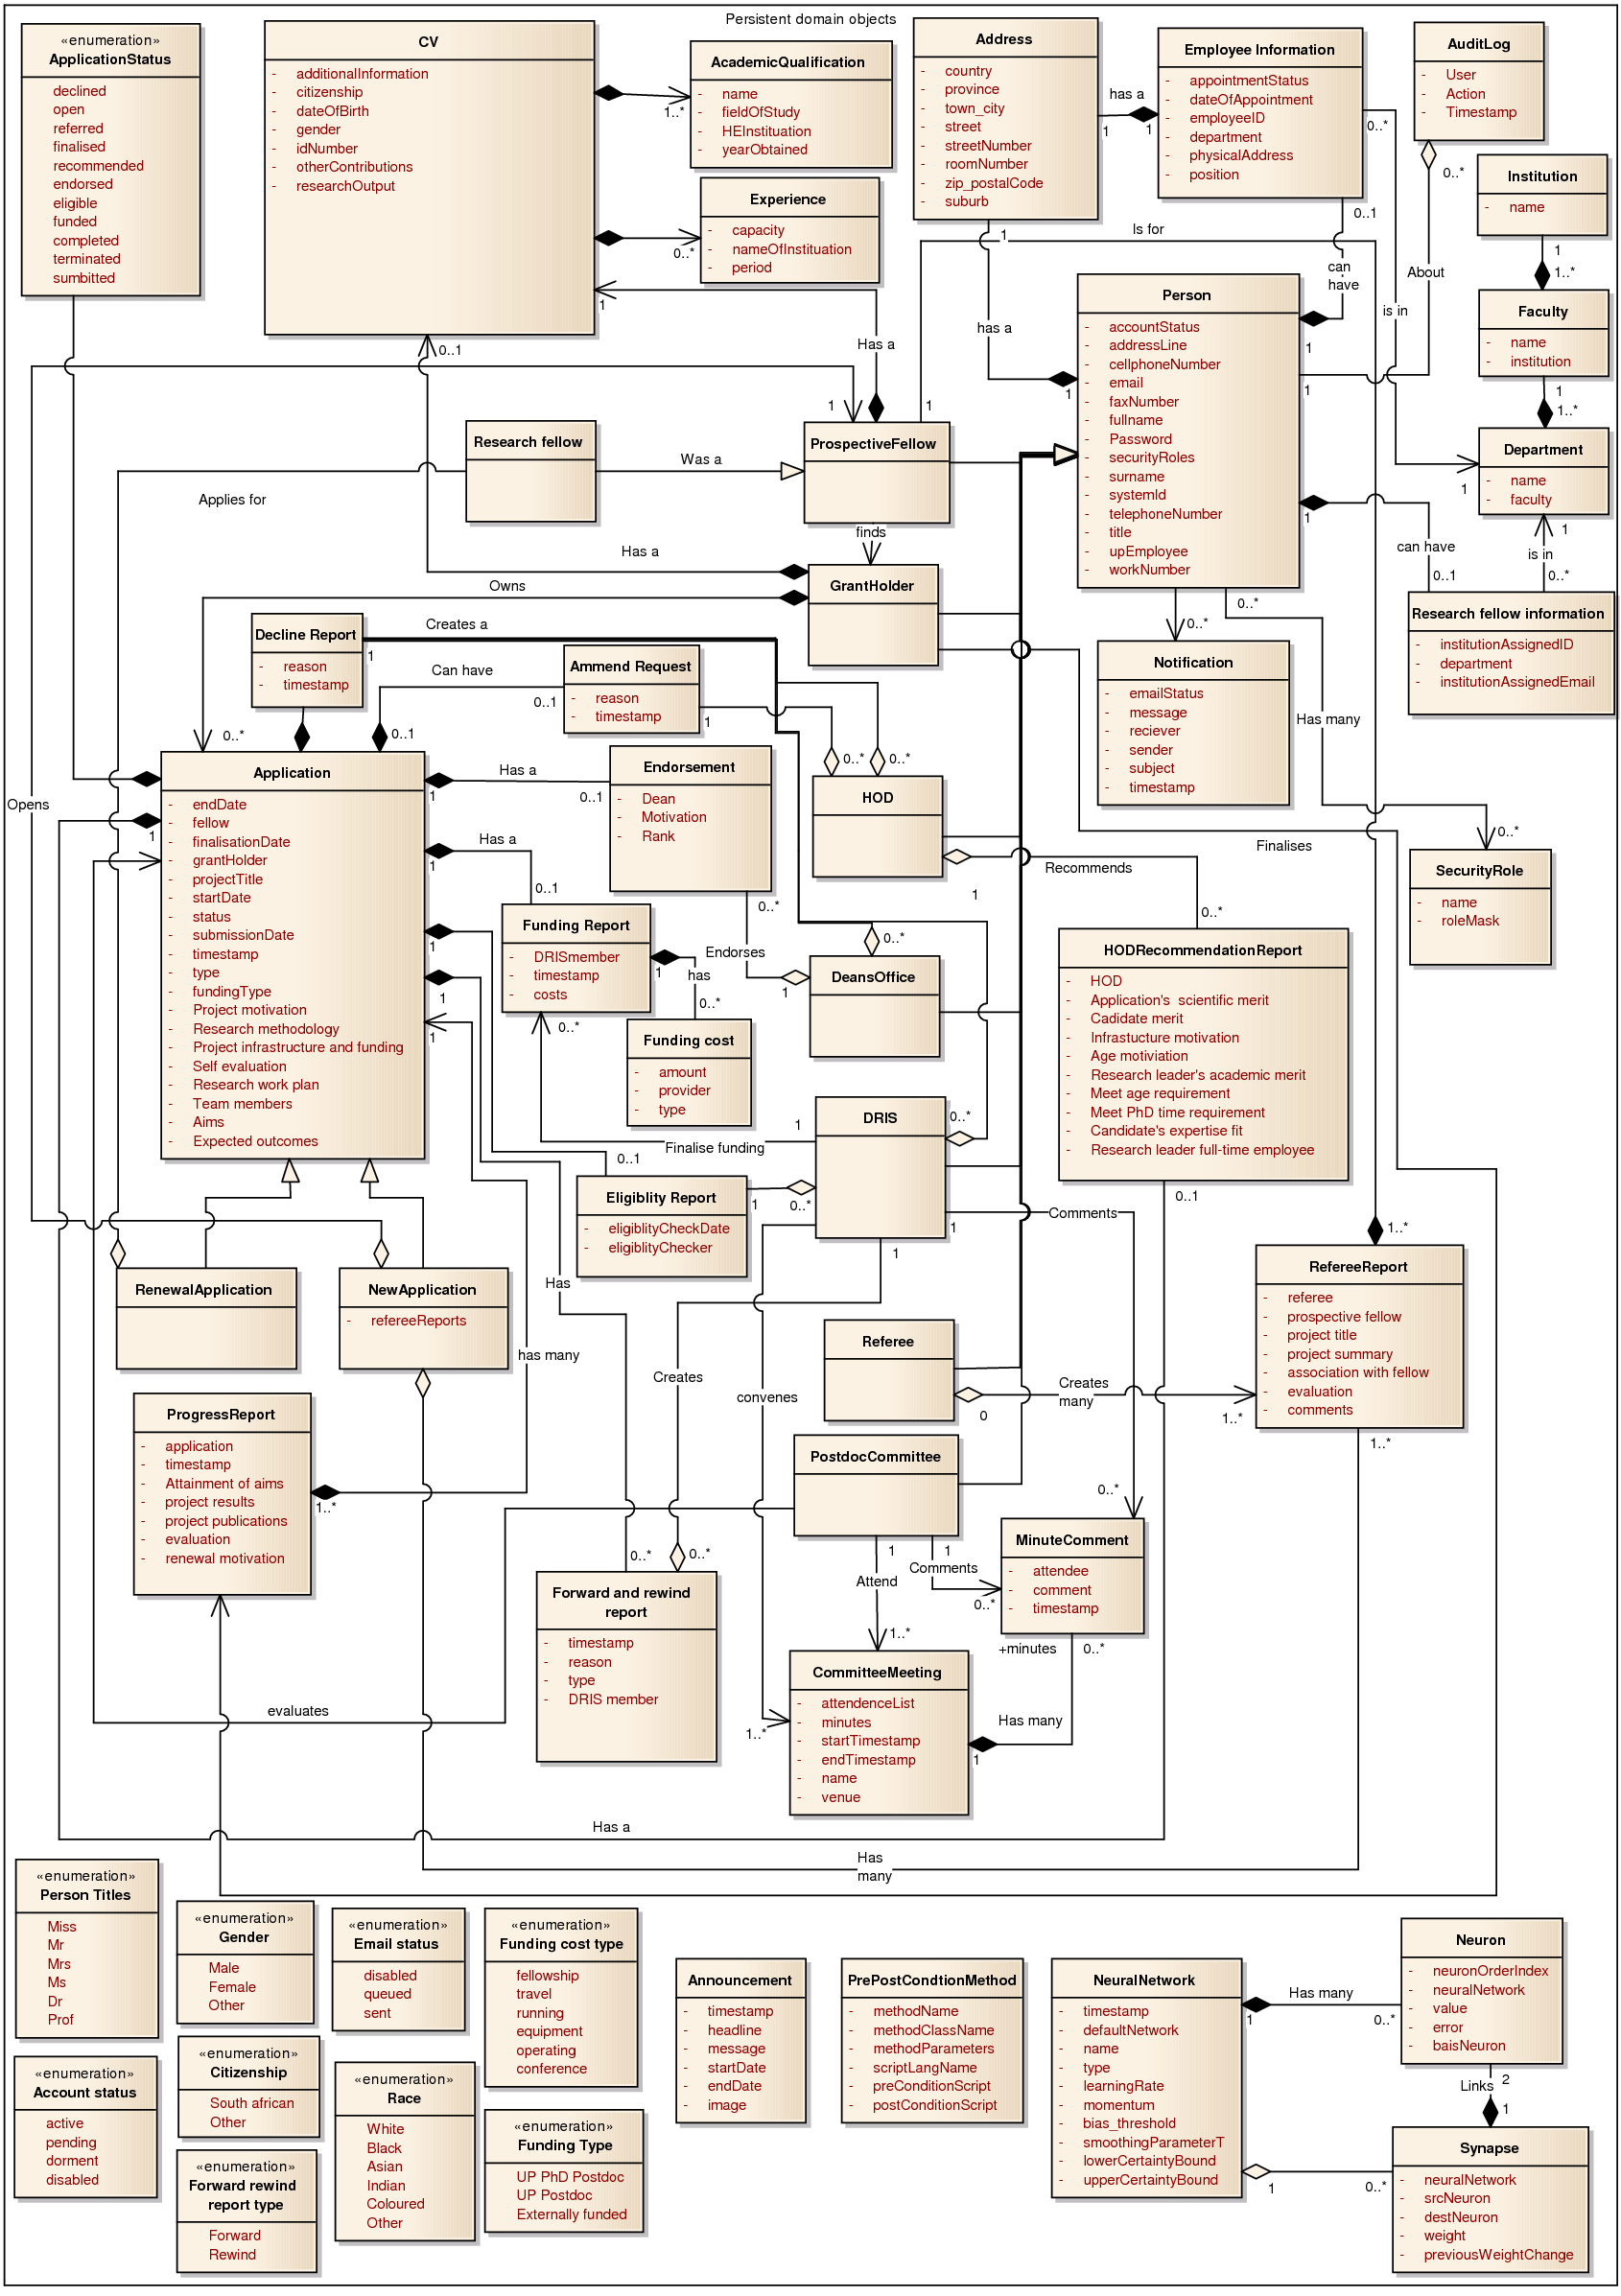
\includegraphics[scale=0.45]{../Images_Docs/Diagrams/DomainObjects/Persistent domain objects1.png}}
\caption{Overview of the data structures and relationships for the persistent domain objects of the
system}
\end{figure}

\newpage
\begin{itemize}
\item \textbf{Person}
This object represents the stakeholders that will make use of the system. All stakeholders will have accounts which they will use to log on to the system, using a unique user id and a predefined or user specified password. The unique user id can either be a Peoplesoft Emplid number or a email address. The person has an associated \textbf{Location} and \textbf{SecurityRole}(s)

\item \textbf{Department}
This object represents the department under which a \textbf{Person} falls in the \textbf{Faculty}. This is used to if they are a \textbf{employee} or \textbf{Research fellow} at the University of Pretoria. This object will no longer be needed if the system is integrated with peoplesoft as it would cause redundancy.

\item \textbf{Faculty}
This object represents the faculty that may exist under an institution. It is used to map the location of a \textbf{Person}. 

\item \textbf{Institution}
This object represents the institutions that may exist in the system. It is used to map the location of a \textbf{Person}. This allows for generic support if the software solution had to be expanded to other universities.

\item \textbf{EmployeeInformation}
This object represents the information regarding the employment of a \textbf{Person} at the University. It also contains the \textbf{Department} under which the \textbf{Person} falls. Also it contains the physical \textbf{Address} of the employee's office. This is made generic for software expansion support.  

\item \textbf{ResearchFellowInformation}
This object represents the CSC's or institution equivalents assigned emplid and the institution's assigned email address for an appointed \textbf{ResearchFellow}. This allows for possible future integration and better user support. Also it stores the \textbf{Department} in the institution to which the fellow was assigned to by the \textbf{DRIS}.

\item \textbf{Address}
This object represents a physical address. Thus it is used to expand and provide location details for a particular physical object or person.  

\item \textbf{SecurityRole}
This object represents a particular security role of a \textbf{Person}. A \textbf{Person} may have many different security roles. The security role can be used as a subtype discriminator for relational database architectures.

\item \textbf{DRIS}
This object represents members of Department of Research and Innovation Support who administers the process.

\item \textbf{FundingReport}
This object represents an \textbf{Application}'s funding costs as decide per the \textbf{DRIS}. It comprises of multiple \textbf{FundingCost}s that provides the various funding inputs from various parties for the particular fund-able costs namely fellowship, travel, running, equipment, operating
and conference.
 
\item \textbf{FundingCost}
This object represents a particular funding input cost for a \textbf{Application} from a particular funder. 

\item \textbf{DeclineReport}
This object represents the report associated with an \textbf{Application} that has been declined by some authority. It contains the creation timestamp, \textbf{Person} responsible and the reason. Only one such report can exist per \textbf{Application}.

\item \textbf{AmmendRequest}
This object represents a Amend request for a \textbf{Application} that is sent by some \textbf{HOD}. It contains the creation timestamp, \textbf{HOD} responsible and the reason. This is used to allow fellow to understand what is wrong with their \textbf{Application} so that they can correct it. There can be multiple such requests associated with an \textbf{Application}.

\item \textbf{EligibilityReport}
This object represents a report associated with an \textbf{Application} that has been checked for eligibility. It contains the check timestamp and \textbf{DRIS} member responsible. It is primary used for auditing. Only one such report can exist per \textbf{Application}.

\item \textbf{ForwardAndRewindReport}
This object represents a report associated with an \textbf{Application} that has been either forwarded or re-winded through a particular set of application stages. This is used to track such actions and the reasons for them. There can be multiple such reports associated with an \textbf{Application}. 
 
\item \textbf{ProspectiveFellow}
This inherited object represents a prospective fellow who is a holder of a PhD obtained in the last five years (or nearing completion of a PhD) or is 40 years or younger and has a PhD. The prospective fellow can open a \textbf{NewApplication}.

\item \textbf{ResearchFellow}
This inherited object represents a research fellow who is a currently a researcher at the University of Pretoria. This object was initially a \textbf{ProspectiveFellow}. The research fellow can apply for a \textbf{RenewalApplication} if their application falls in their renewal time frame.

\item \textbf{GrantHolder}
This inherited object represents a grant holder who can be a rated researcher by the NRF or not. The system should not require the CV's of A and B rated researchers to be added to the system. The reason for this is that the CV's of such researchers can be easily obtained from the NRF and tend to be very long. A grant holder is the supervisor for a or many \textbf{ProspectiveFellow}(s) or \textbf{ResearchFellow}(s) and owns the \textbf{Application} of the \textbf{ProspectiveFellow}(s) or \textbf{ResearchFellow}(s).

\item \textbf{HOD}
This inherited object represents a HOD of a particular department. The HOD creates the recommendation reports for \textbf{Application}(s) they consider to meet their requirements.\\

\item \textbf{HODRecommandationReport}
This inherited object represents a recommendation report highlighting the reasons to why the \textbf{Application} of a \textbf{ProspectiveFellow} or \textbf{ResearchFellow} is needed by the department.

\item \textbf{Deans Office}
The Dean's office object represents the relevant faculty's Dean and Deputy Dean. The Dean's Office creates the \textbf{Endorsement} for any the \textbf{Application} that is approved by them.

\item \textbf{Endorsement}
This object represents the endorsement of an \textbf{Application} of a \textbf{ProspectiveFellow} or \textbf{ResearchFellow} and contains the rank in comparison to other pending \textbf{Application}(s) with a \textbf{Endorsement}.

\item \textbf{Referee}
This inherited object represents the referees of any \textbf{ProspectiveFellow} and is responsible for creating \textbf{RefereeReport} regarding the \textbf{ProspectiveFellow}.

\item \textbf{RefereeReport}
This object represents the referral report from an identified referee of a \textbf{ProspectiveFellow}.

\item \textbf{PostDocCommittee}
This inherited object represents the individual members of the post-doctoral committee who approves all available \textbf{Applications} during committee meetings and records the \textbf{Minutes} of the meeting.

\item \textbf{CommitteeMeeting}
This object represents a meeting of the \textbf{PostDocCommittee} convened by the \textbf{DRIS} that will be review the \textbf{Applications} and will evaluate each. This object contains the attendance list, date and time convened and the \textbf{MinuteComment}s of the meeting.

\item \textbf{MinuteComment}
This object represents a comment made by a \textbf{PostDocCommittee} member during a \textbf{CommitteeMeeting}.

\item \textbf{Application}
This object represents an applications and will contain the information of \textbf{ProspectiveFellow} or \textbf{ResearchFellow} and \textbf{GrantHolder} who owns it. The object holds the status of the application and any project information. As well as the \textbf{HODRecommandationReport} of a \textbf{HOD} and \textbf{Endorsement} from a \textbf{DeansOffice}. It further holds the \textbf{EligibilityReport} and \textbf{FundingReport} from the \textbf{DRIS}. If the application is declined the \textbf{DeclineReport} is associated with the application. The application object can also hold multiple \textbf{AmmendRequest}s if any such requests are created. All the \textbf{ProgressReport}s created by the \textbf{ResearchFellow} are also contained in the application. Lastly if the application forwarded or re-winded then the associated \textbf{Forward rewind report}s are also contained by the application 

\item \textbf{NewApplication}
This inherited object represents new application for a \textbf{ProspectiveFellow} who is currently not a fellow in the system. Also it holds any \textbf{RefereeReport}(s) that has been created for the application.

\item \textbf{RenewalApplication}
This inherited object represents renewal application for a \textbf{ProspectiveFellow} who is a fellow in the system. Also it holds the \textbf{ProgressReport} that has been created for the application.

\item \textbf{ProgressReport}
This object represents the periodical report on the research that the \textbf{ResearchFellow} has done for the particular period in the duration of their fellowship. These reports are completed on an annual bases.

\item \textbf{CV}
This object represents a CV and contains all the information such as personal details, \textbf{AcademicQualification}(s), \textbf{Experience} regarding a \textbf{GrantHolder} or \textbf{ProspectiveFellow} in the system.

\item \textbf{AcademicQualification}
This object represents a academic qualification and the information regarding it such as the qualification name, field, where it was obtained and when it was obtained.

\item \textbf{Experience}
This object represents a work experience and the information regarding it such as the capacity of the work, where this work was done and when it was done.

\item \textbf{Notification}
This object represents a email or internal message sent by a user to a user via the system. The system itself may also seen as a user with regards to the sender of such notification. It consists of the actual message, subject, timestamp and email status. 

\item \textbf{AuditLog}
This object represents a audit log that stores all the actions of all users within the system. Each entry records the action, who committed the action as well as at what time the action was committed.


\end{itemize}

\newpage
\subsubsection{Non-Persistent domain objects}
These domain objects represent those domain objects that are not stored in some form of persistent data store and exist with in the runtime of the software solution.

\begin{figure}[H]
\centering	
\framebox{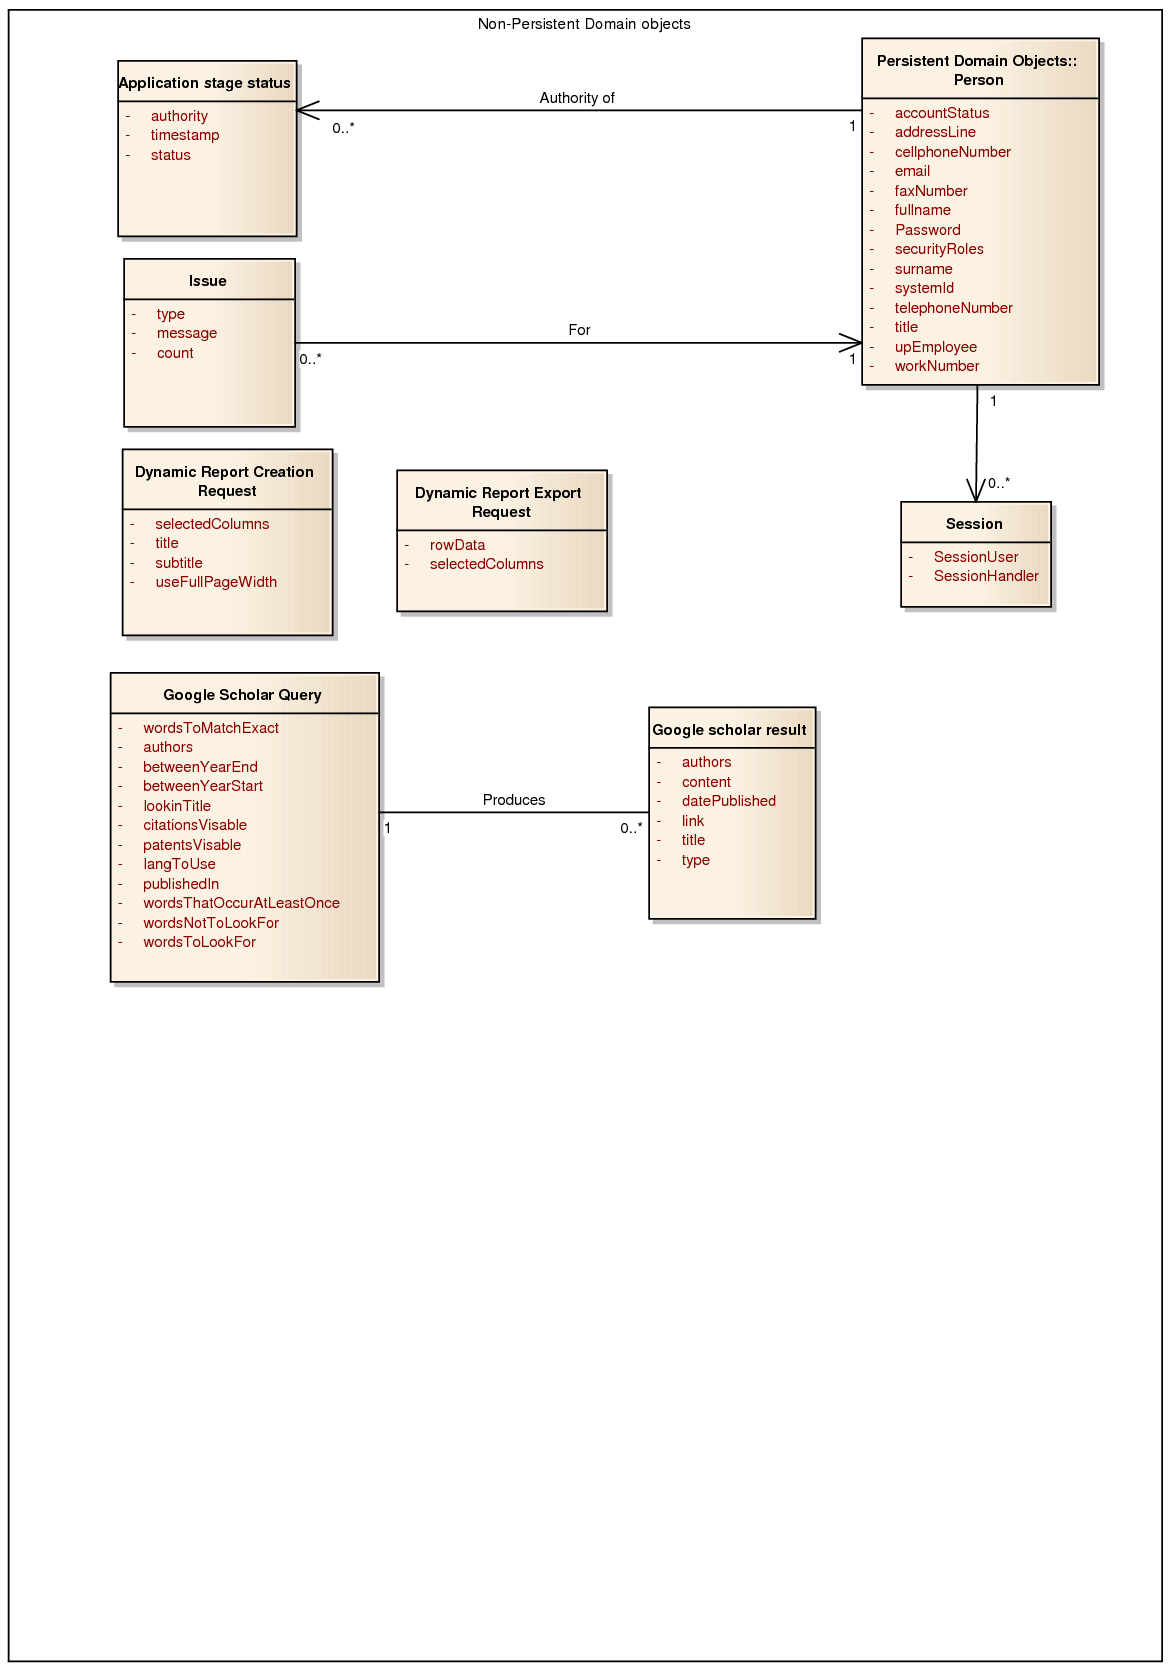
\includegraphics[scale=0.65]{../Images_Docs/Diagrams/DomainObjects/Non-Persistent domain objects1.png}}
\caption{Overview of the data structures and relationships for the non-persistent domain objects of the
system}
\end{figure}

\newpage
\begin{itemize}
\item \textbf{ApplicationStageStatus}
This object represents a stage change that has occurred for a particular \textbf{Application} which was caused by a \textbf{Person} in the system.

\item \textbf{Issue}
This object represents an outstanding issue for a particular \textbf{Person} in the system. It consist of a message and the number of such instances.

\item \textbf{Session}
This object represents a the details of a currently active session on the system. It contains the user (\textbf{Person}) and the link to the system's session management system's record. This object will be used through out the system for auditing and authentication.

\item \textbf{DynamicReportCreationRequest}
This object represents a report creation request that a \textbf{DRIS} member is making to the system. It contains all the configuration information needed to generate a report.

\item \textbf{DynamicReportExportRequest}
This object represents a report export request that a \textbf{DRIS} member is making to the system. It contains all the configuration and data information needed to generate the report to a particular format.

\item \textbf{GoogleScholarQuery}
This object represents a query that is made to the Google Scholar website by the system.

\item \textbf{GoogleScholarResult}
This object represents a result returned by one a \textbf{GoogleScholarQuery} to the Google scholar service.

\end{itemize} 

\newpage
\subsection{Data flow diagrams}
\begin{figure}[H]
\centering	
\framebox{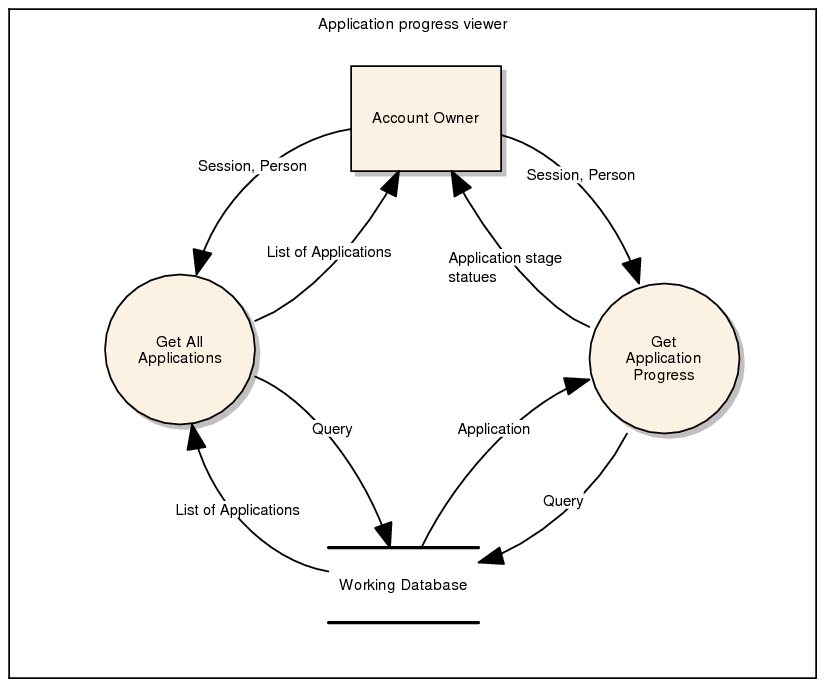
\includegraphics[scale=0.75]{../Images_Docs/Diagrams/Data Flow/ApplicationProgress1.png}}
\caption{Data Flow for Application progress viewer services}
\end{figure}

\begin{figure}[H]
\centering	
\framebox{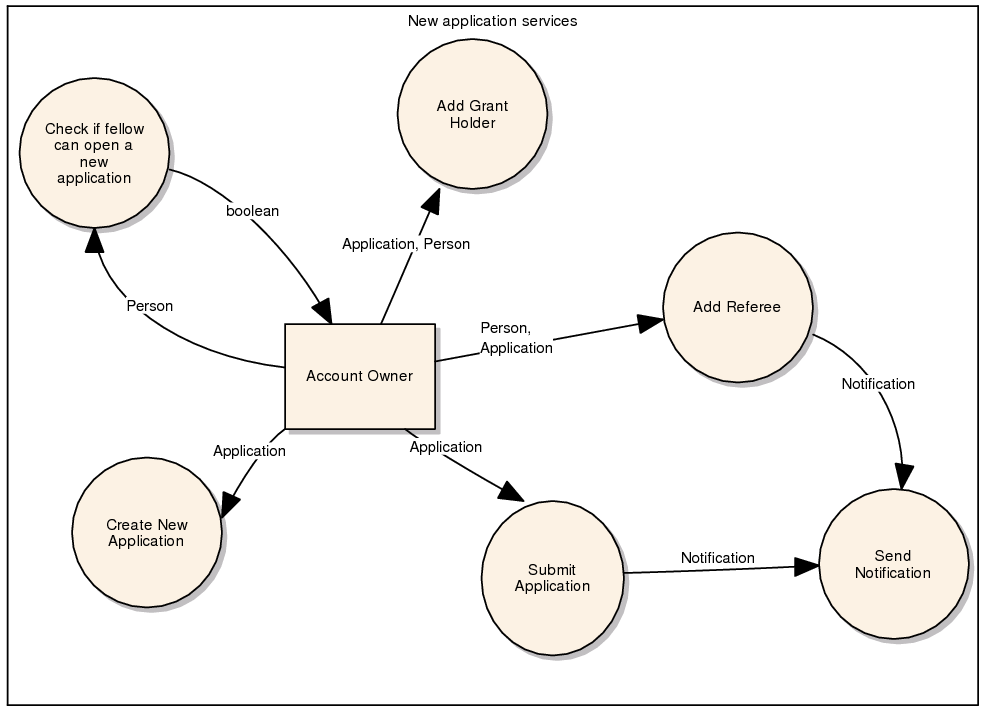
\includegraphics[scale=0.7]{../Images_Docs/Diagrams/Data Flow/NewApplication1.png}}
\caption{Data Flow for New Application services}
\end{figure}

\begin{figure}[H]
\centering	
\framebox{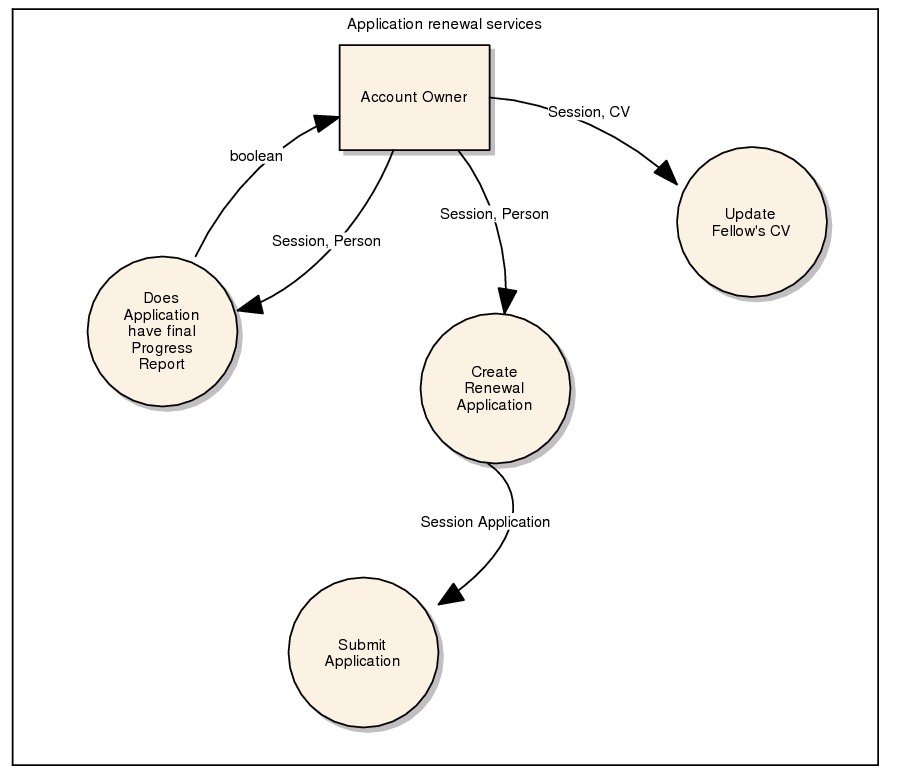
\includegraphics[scale=0.75]{../Images_Docs/Diagrams/Data Flow/ApplicationRenewal1.png}}
\caption{Data Flow for Application Renewal services}
\end{figure}

\begin{figure}[H]
\centering	
\framebox{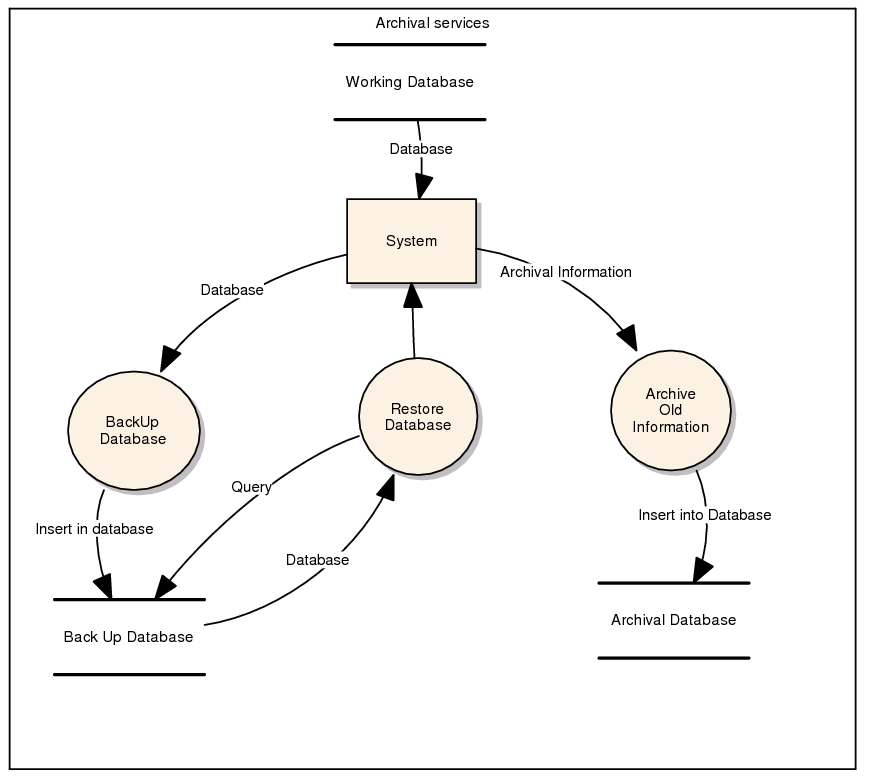
\includegraphics[scale=0.75]{../Images_Docs/Diagrams/Data Flow/ArchivalService1.png}}
\caption{Data Flow for Archival Service services}
\end{figure}

\begin{figure}[H]
\centering	
\framebox{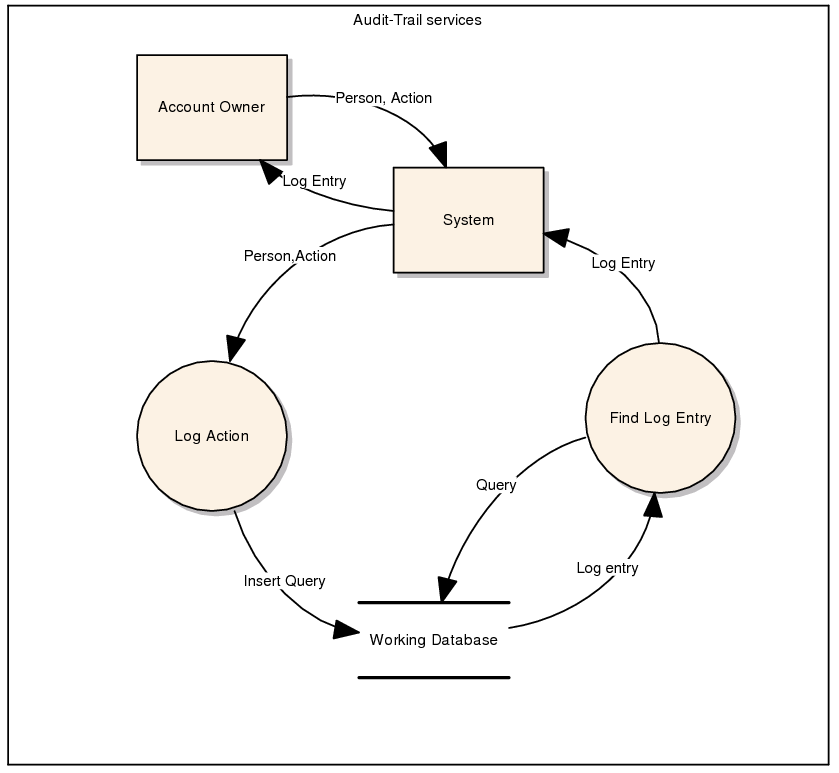
\includegraphics[scale=0.8]{../Images_Docs/Diagrams/Data Flow/AuditTrail1.png}}
\caption{Data Flow for Audit Trail services}
\end{figure}

\begin{figure}[H]
\centering	
\framebox{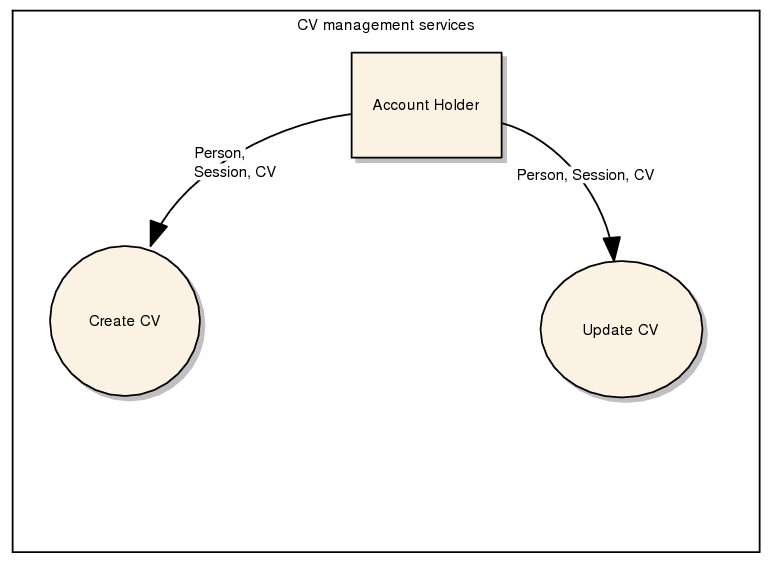
\includegraphics[scale=0.8]{../Images_Docs/Diagrams/Data Flow/CVManagement1.png}}
\caption{Data Flow CV Management services}
\end{figure}

\begin{figure}[H]
\centering	
\framebox{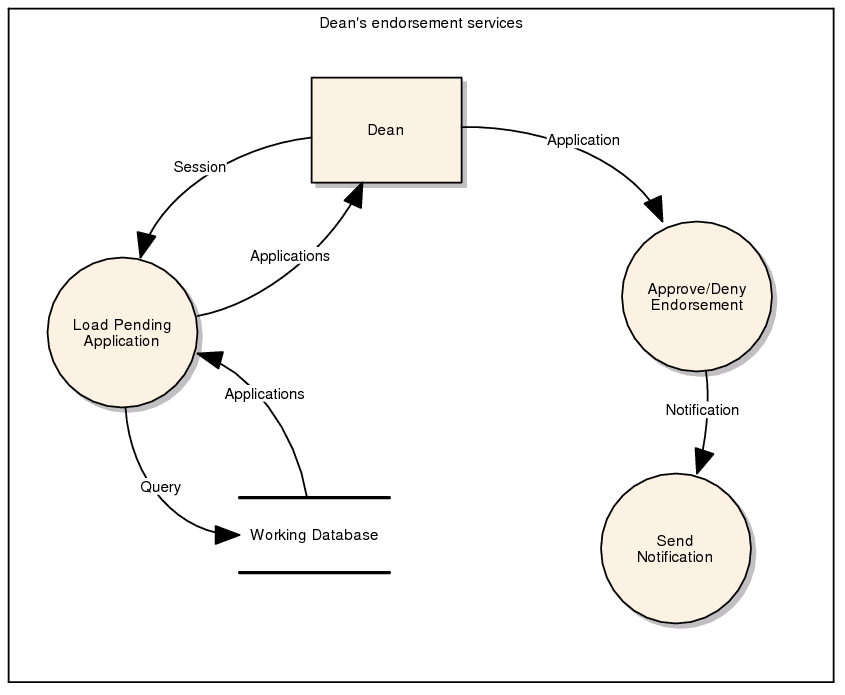
\includegraphics[scale=0.8]{../Images_Docs/Diagrams/Data Flow/DeansEndorsement1.png}}
\caption{Data Flow for Dean's Endorsement services}
\end{figure}

\begin{figure}[H]
\centering	
\framebox{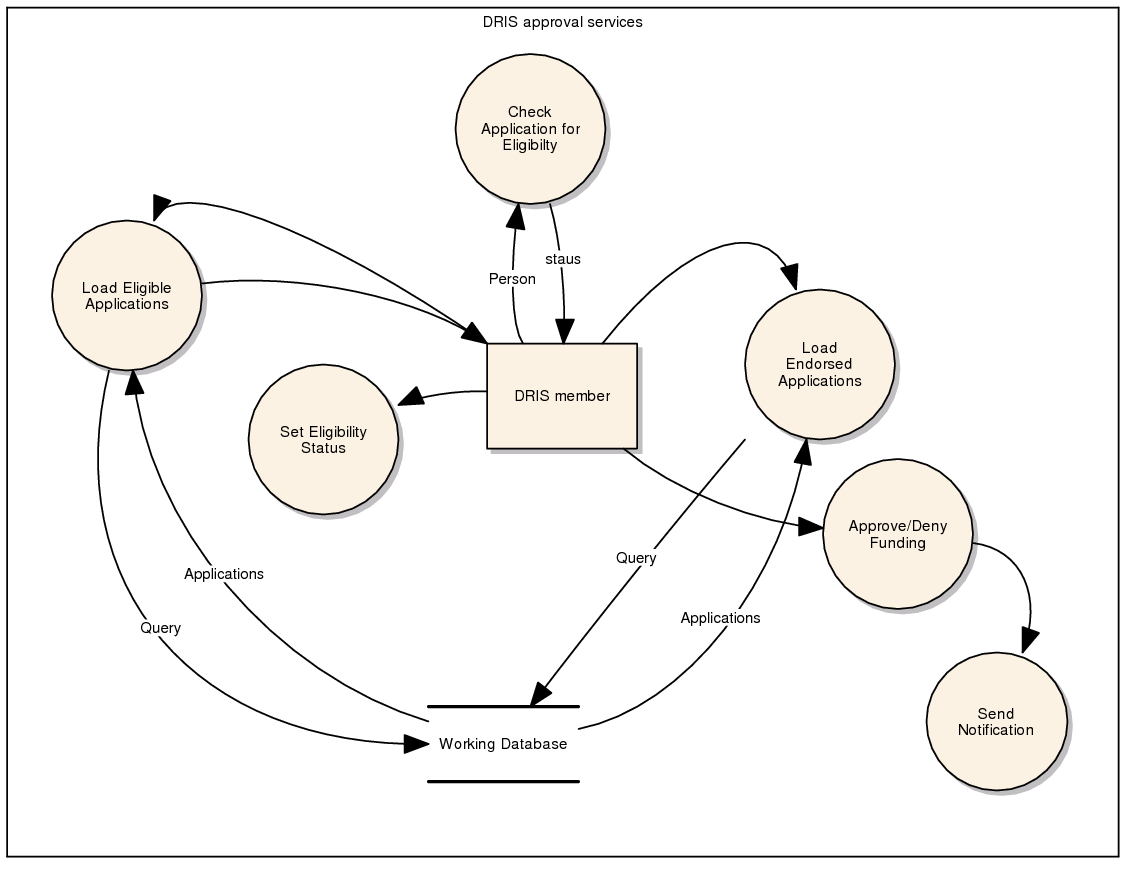
\includegraphics[scale=0.7]{../Images_Docs/Diagrams/Data Flow/DRISApproval1.png}}
\caption{Data Flow for DRIS Approval services}
\end{figure}

\begin{figure}[H]
\centering	
\framebox{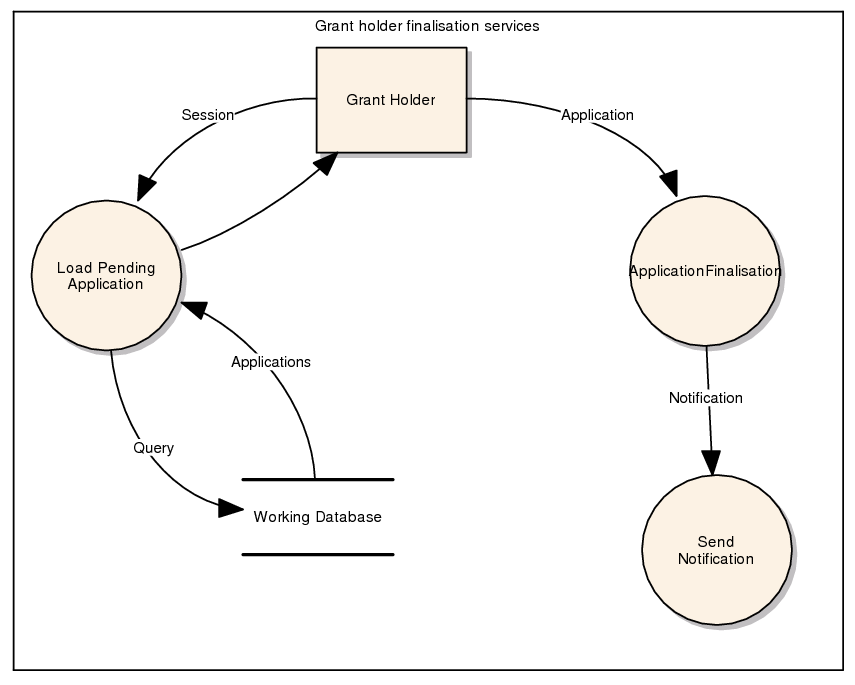
\includegraphics[scale=0.8]{../Images_Docs/Diagrams/Data Flow/GrantHolderFinalisation1.png}}
\caption{Data Flow for Grant Holder Finalisation services}
\end{figure}

\begin{figure}[H]
\centering	
\framebox{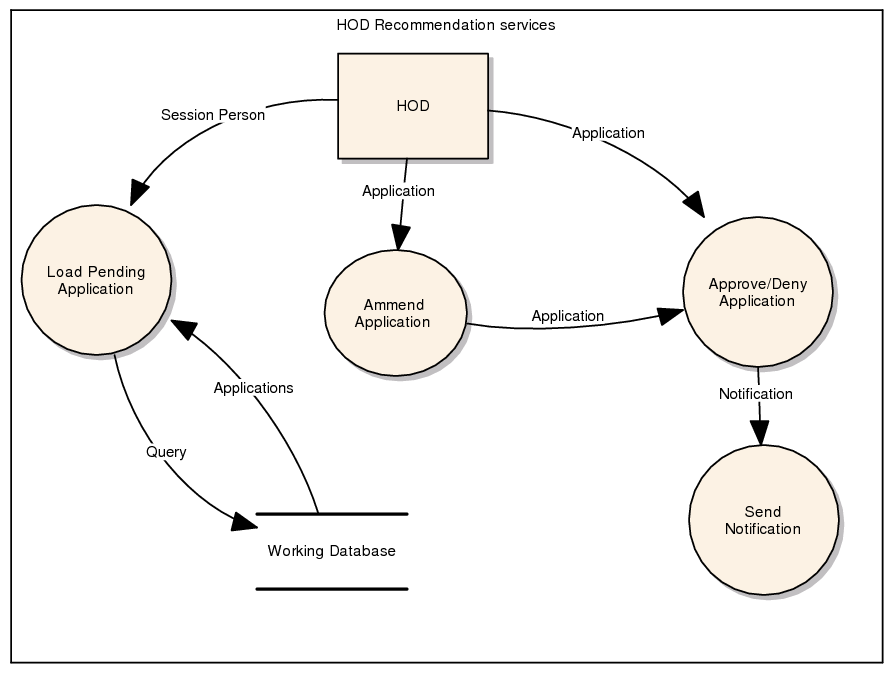
\includegraphics[scale=0.8]{../Images_Docs/Diagrams/Data Flow/HODRecommendation1.png}}
\caption{Data Flow for HOD Recommendation services}
\end{figure}

\begin{figure}[H]
\centering	
\framebox{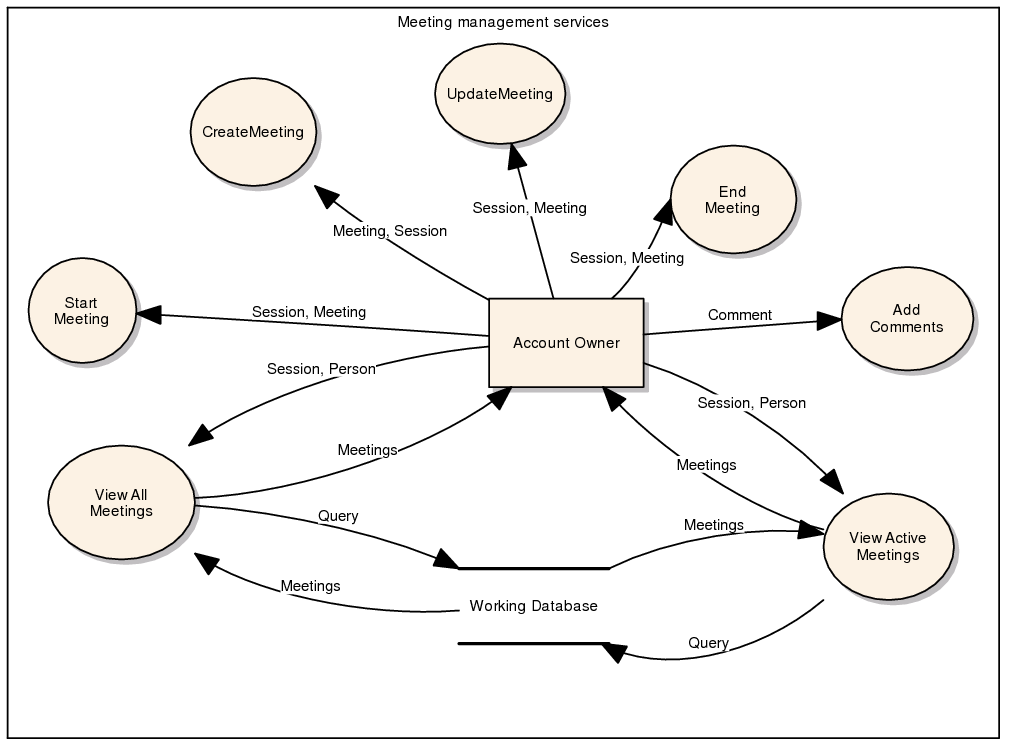
\includegraphics[scale=0.7]{../Images_Docs/Diagrams/Data Flow/MeetingManagement1.png}}
\caption{Data Flow for Meeting Management services}
\end{figure}

\begin{figure}[H]
\centering	
\framebox{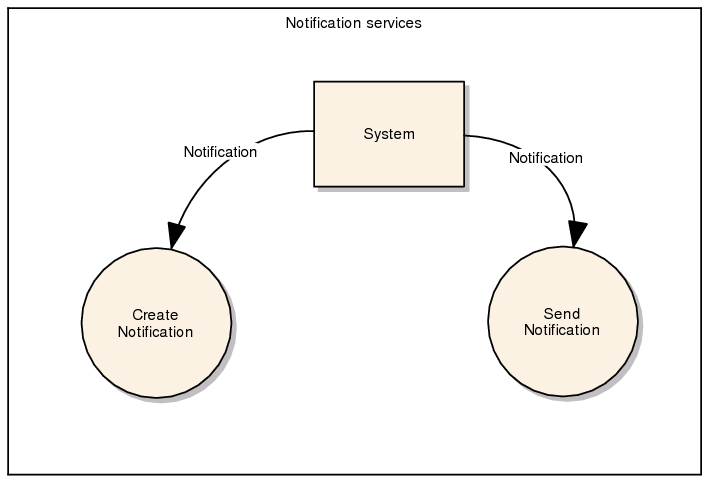
\includegraphics[scale=0.8]{../Images_Docs/Diagrams/Data Flow/NotificationService1.png}}
\caption{Data Flow for Notification Service services}
\end{figure}

\begin{figure}[H]
\centering	
\framebox{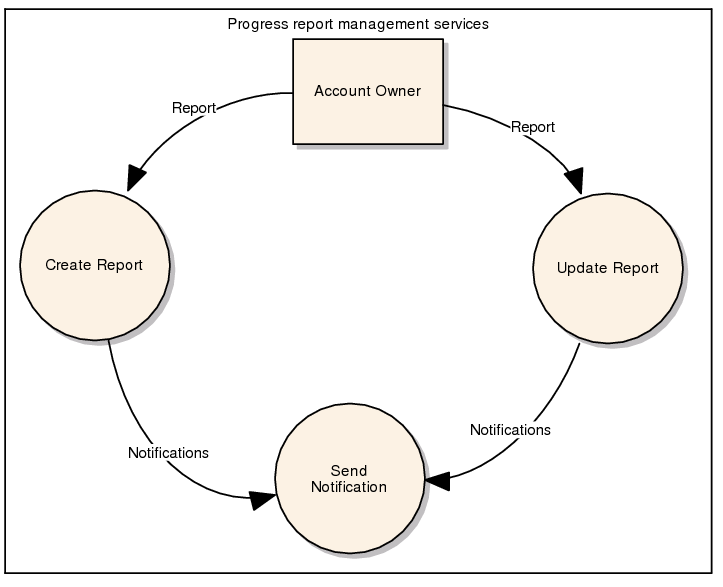
\includegraphics[scale=0.8]{../Images_Docs/Diagrams/Data Flow/ProgressReport1.png}}
\caption{Data Flow for Progress Reports services}
\end{figure}

\begin{figure}[H]
\centering	
\framebox{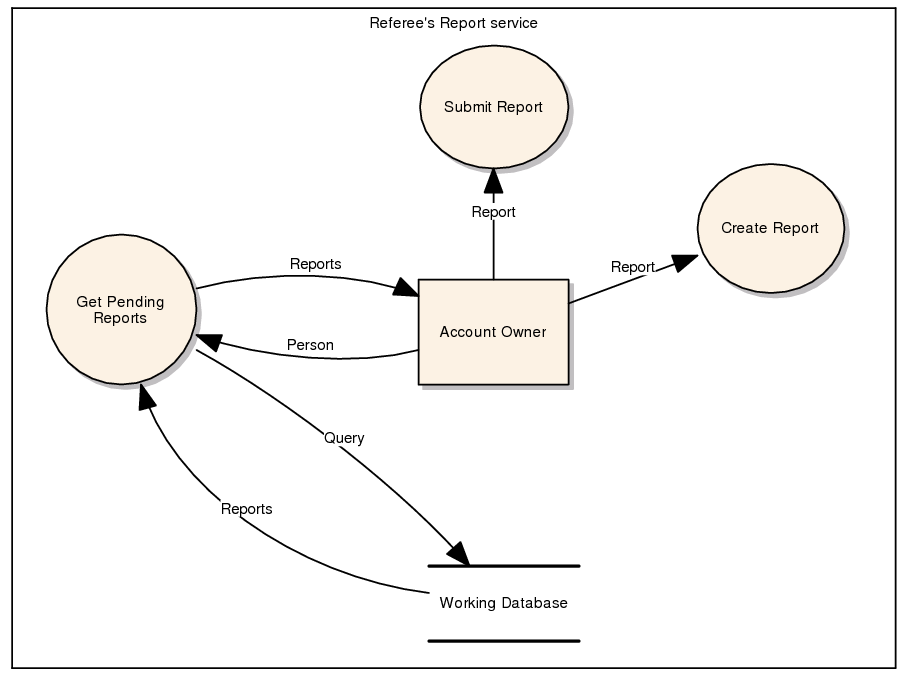
\includegraphics[scale=0.8]{../Images_Docs/Diagrams/Data Flow/RefereeReport1.png}}
\caption{Data Flow for Referee Report services}
\end{figure}

\begin{figure}[H]
\centering	
\framebox{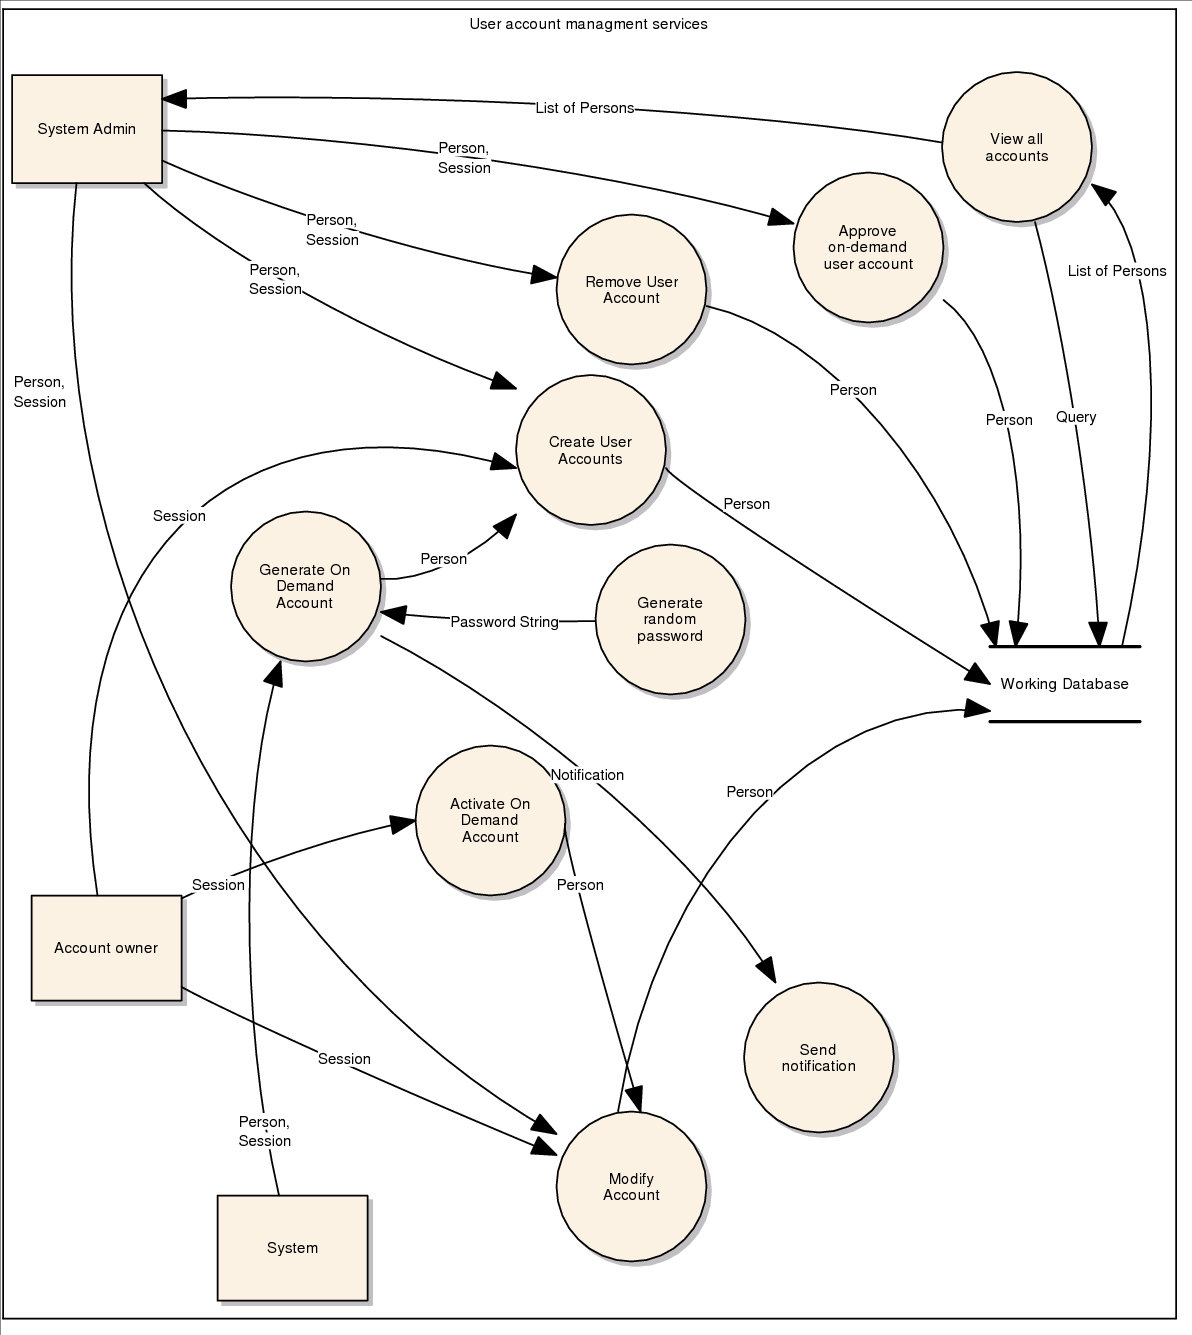
\includegraphics[scale=0.8]{../Images_Docs/Diagrams/Data Flow/UserAccount1.png}}
\caption{Data Flow for User Account Management services}
\end{figure}

\begin{figure}[H]
\centering	
\framebox{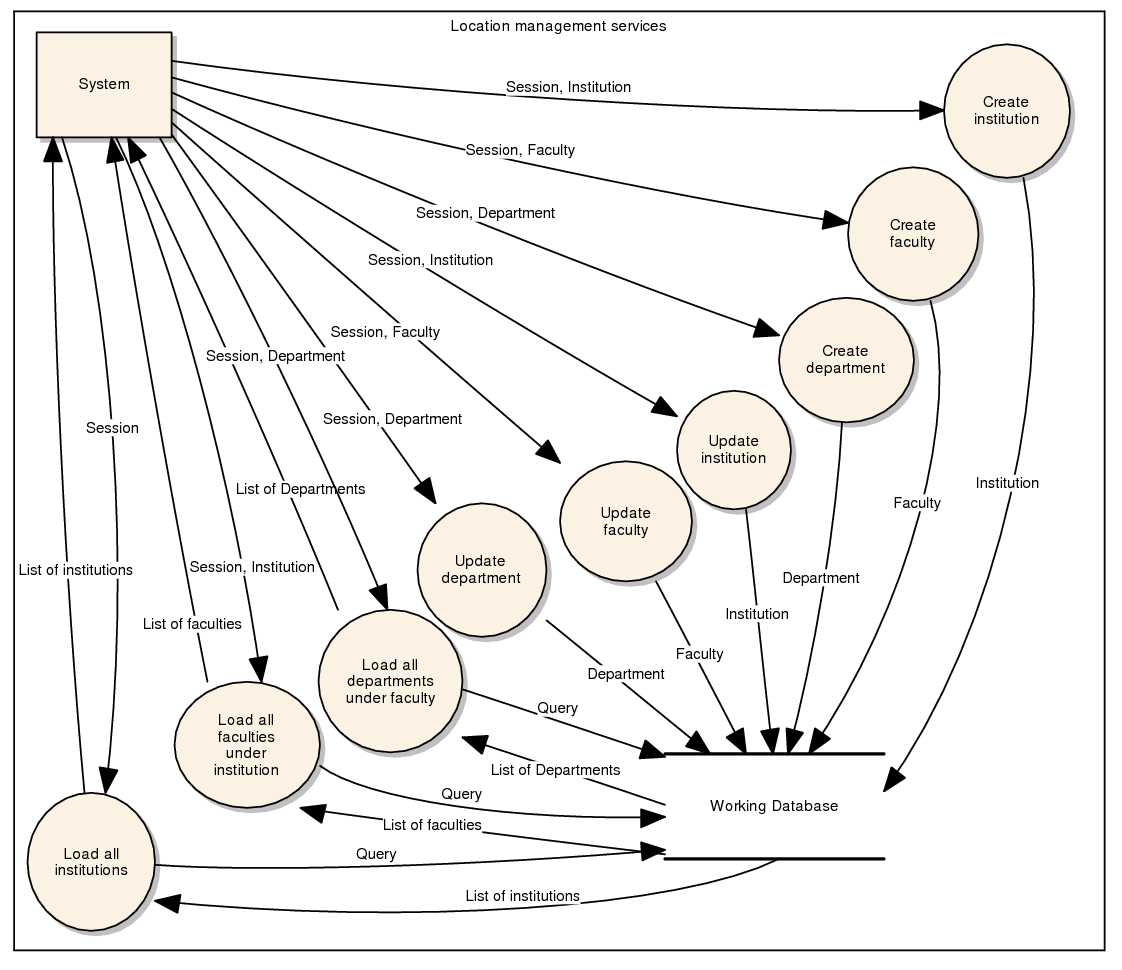
\includegraphics[scale=0.85]{../Images_Docs/Diagrams/Data Flow/Location management services1.png}}
\caption{Data Flow for Location management services}
\end{figure}

\begin{figure}[H]
\centering	
\framebox{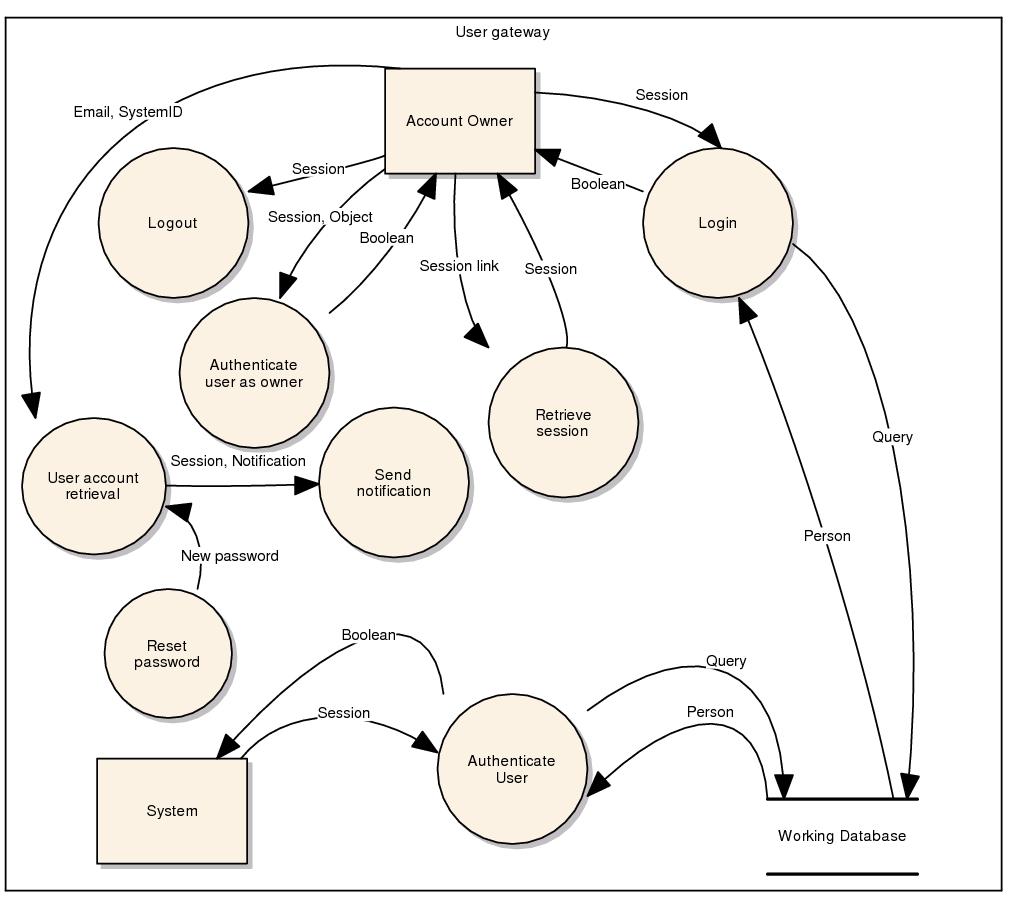
\includegraphics[scale=0.7]{../Images_Docs/Diagrams/Data Flow/UserGateway1.png}}
\caption{Data Flow for User Gateway.}
\end{figure}

\begin{figure}[H]
\centering	
\framebox{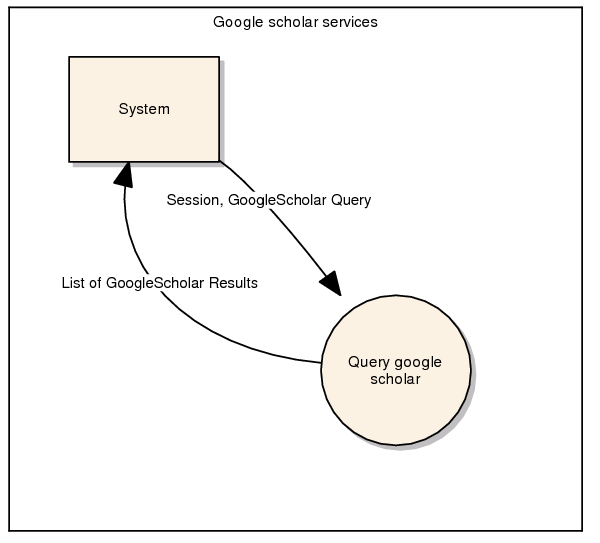
\includegraphics[scale=0.8]{../Images_Docs/Diagrams/Data Flow/Google scholar services1.png}}
\caption{Data Flow for Google scholar services}
\end{figure}

\begin{figure}[H]
\centering	
\framebox{\includegraphics[scale=0.75]{../Images_Docs/Diagrams/Data Flow/Forward and rewind services1.png}}
\caption{Data Flow for Forward and rewind services}
\end{figure}

\begin{figure}[H]
\centering	
\framebox{\includegraphics[scale=0.8]{../Images_Docs/Diagrams/Data Flow/Reporting1.png}}
\caption{Data Flow for Reporting Service services}
\end{figure}

\begin{figure}[H]
\centering	
\framebox{\includegraphics[scale=0.8]{../Images_Docs/Diagrams/Data Flow/Announcement services1.png}}
\caption{Data Flow for Announcement services}
\end{figure}

\begin{figure}[H]
\centering	
\framebox{\includegraphics[scale=0.8]{../Images_Docs/Diagrams/Data Flow/Application import services1.png}}
\caption{Data Flow for Application import services}
\end{figure}


\vspace{0.2in}
\newpage
\subsection{Process specifications}
\vspace{0.2in}

\begin{figure}[H]
\centering	
\framebox{\includegraphics[scale=0.7]{../Images_Docs/Diagrams/Process specs/Login user.jpg}}
\caption{Activity diagram of the Login user use case.}
\end{figure}

\begin{figure}[H]
\centering	
\framebox{\includegraphics[scale=0.65]{../Images_Docs/Diagrams/Process specs/Generate user on-demand account.jpg}}
\caption{Activity diagram of the Generate user on-demand account use case.}
\end{figure}


\begin{figure}[H]
\centering	
\framebox{\includegraphics[scale=1]{../Images_Docs/Diagrams/Process specs/Activate user on-demand account.jpg}}
\caption{Activity diagram of the Activate user on-demand account use case.}
\end{figure}

\begin{figure}[H]
\centering	
\framebox{\includegraphics[scale=1]{../Images_Docs/Diagrams/Process specs/Authenticate user.jpg}}
\caption{Activity diagram of the Authenticate user use case.}
\end{figure}

\begin{figure}[H]
\centering	
\framebox{\includegraphics[scale=1]{../Images_Docs/Diagrams/Process specs/User account retrieval.jpg}}
\caption{Activity diagram of the User account retrieval use case.}
\end{figure}

\begin{figure}[H]
\centering	
\framebox{\includegraphics[scale=1]{../Images_Docs/Diagrams/Process specs/Load pending applications.jpg}}
\caption{Activity diagram of the Load pending applications use case.}
\end{figure}

%%%%%%%%%%%%%%%%%%%%%%%%%%%%%%%%%%%%%%%%%%%%%%%%%%%%%%%%%%%%%%%%%%%%%%%%%%%%%%%%%%%%%%%%%%%%%%%%%%%%%%%%%%%%%%%%%%%%%%%%%%%%%%%%%%%%

\begin{figure}[H]
\centering	
\framebox{\includegraphics[scale=0.65]{../Images_Docs/Diagrams/Activity Diagrams/AnnouncementManagement/createAnnouncement.png}}
\caption{Activity diagram of the create anouncement use case.}
\end{figure}

\begin{figure}[H]
\centering	
\framebox{\includegraphics[scale=0.65]{../Images_Docs/Diagrams/Activity Diagrams/AnnouncementManagement/loadAllActiveAnnouncements.png}}
\caption{Activity diagram of the load all anouncements use case.}
\end{figure}


\begin{figure}[H]
\centering	
\framebox{\includegraphics[scale=0.65]{../Images_Docs/Diagrams/Activity Diagrams/AnnouncementManagement/loadAllPendingAnnouncements.png}}
\caption{Activity diagram of the load all pending anouncements use case.}
\end{figure}


\begin{figure}[H]
\centering	
\framebox{\includegraphics[scale=0.65]{../Images_Docs/Diagrams/Activity Diagrams/AnnouncementManagement/removeAnnouncement.png}}
\caption{Activity diagram of the remove anouncement use case.}
\end{figure}


\begin{figure}[H]
\centering	
\framebox{\includegraphics[scale=0.65]{../Images_Docs/Diagrams/Activity Diagrams/AnnouncementManagement/updateAnnouncement.png}}
\caption{Activity diagram of the update anouncement use case.}
\end{figure}


%%%%%%%%%%%%%%%%%%%%%%%%%%%%%%%%%%%%%%%%%%%%%%%%%%%%%%%%%%%%%%%%%%%%%%%%%%%%%%%%%%%%%%%%%%%%%%%%%%%%%%%%%%%%%%%%%%%%%%%%%%%%%%%%%%%%

\begin{figure}[H]
\centering	
\framebox{\includegraphics[scale=0.25]{../Images_Docs/Diagrams/Activity Diagrams/ApplicationProgressViewer/Get All Applications.jpg}}
\caption{Activity diagram of the Get All Applications use case.}
\end{figure}

\begin{figure}[H]
\centering	
\framebox{\includegraphics[scale=0.25]{../Images_Docs/Diagrams/Activity Diagrams/ApplicationProgressViewer/View application progress.jpg}}
\caption{Activity diagram of the View application progress use case.}
\end{figure}

%%%%%%%%%%%%%%%%%%%%%%%%%%%%%%%%%%%%%%%%%%%%%%%%%%%%%%%%%%%%%%%%%%%%%%%%%%%%%%%%%%%%%%%%%%%%%%%%%%%%%%%%%%%%%%%%%%%%%%%%%%%%%%%%%%%%

\begin{figure}[H]
\centering	
\framebox{\includegraphics[scale=0.25]{../Images_Docs/Diagrams/Activity Diagrams/ApplicationRenewalService/Create Final Progress Report For Application.jpg}}
\caption{Activity diagram of the Create Final Progress Report For Application use case.}
\end{figure}

\begin{figure}[H]
\centering	
\framebox{\includegraphics[scale=0.25]{../Images_Docs/Diagrams/Activity Diagrams/ApplicationRenewalService/Create renewal Application.jpg}}
\caption{Activity diagram of the Create renewal Application use case.}
\end{figure}

\begin{figure}[H]
\centering	
\framebox{\includegraphics[scale=0.25]{../Images_Docs/Diagrams/Activity Diagrams/ApplicationRenewalService/Does Application Have Final Progress Report.jpg}}
\caption{Activity diagram of the Does Application Have Final Progress Report use case.}
\end{figure}

\begin{figure}[H]
\centering	
\framebox{\includegraphics[scale=0.25]{../Images_Docs/Diagrams/Activity Diagrams/ApplicationRenewalService/Get Renewable Applications for Fellow.jpg}}
\caption{Activity diagram of the Get Renewable Applications for Fellow use case.}
\end{figure}

%%%%%%%%%%%%%%%%%%%%%%%%%%%%%%%%%%%%%%%%%%%%%%%%%%%%%%%%%%%%%%%%%%%%%%%%%%%%%%%%%%%%%%%%%%%%%%%%%%%%%%%%%%%%%%%%%%%%%%%%%%%%%%%%%%%%

\begin{figure}[H]
\centering	
\framebox{\includegraphics[scale=0.25]{../Images_Docs/Diagrams/Activity Diagrams/CV Management Service/Create CV.jpg}}
\caption{Activity diagram of the Create CV use case.}
\end{figure}

\begin{figure}[H]
\centering	
\framebox{\includegraphics[scale=0.25]{../Images_Docs/Diagrams/Activity Diagrams/CV Management Service/Update CV.jpg}}
\caption{Activity diagram of the Update CV use case.}
\end{figure}

%%%%%%%%%%%%%%%%%%%%%%%%%%%%%%%%%%%%%%%%%%%%%%%%%%%%%%%%%%%%%%%%%%%%%%%%%%%%%%%%%%%%%%%%%%%%%%%%%%%%%%%%%%%%%%%%%%%%%%%%%%%%%%%%%%%%

\begin{figure}[H]
\centering	
\framebox{\includegraphics[scale=0.25]{../Images_Docs/Diagrams/Activity Diagrams/Dean Endorsement/Deny Application.jpg}}
\caption{Activity diagram of the Deny Application use case.}
\end{figure}

\begin{figure}[H]
\centering	
\framebox{\includegraphics[scale=0.25]{../Images_Docs/Diagrams/Activity Diagrams/Dean Endorsement/Endorse Application.jpg}}
\caption{Activity diagram of the Endorse Application use case.}
\end{figure}

%%%%%%%%%%%%%%%%%%%%%%%%%%%%%%%%%%%%%%%%%%%%%%%%%%%%%%%%%%%%%%%%%%%%%%%%%%%%%%%%%%%%%%%%%%%%%%%%%%%%%%%%%%%%%%%%%%%%%%%%%%%%%%%%%%%%

\begin{figure}[H]
\centering	
\framebox{\includegraphics[scale=0.25]{../Images_Docs/Diagrams/Activity Diagrams/DRISApprovalService/Approve Funding.jpg}}
\caption{Activity diagram of the Approve Funding use case.}
\end{figure}

\begin{figure}[H]
\centering	
\framebox{\includegraphics[scale=0.25]{../Images_Docs/Diagrams/Activity Diagrams/DRISApprovalService/Check Appligibilty.jpg}}
\caption{Activity diagram of the Check Appligibilty use case.}
\end{figure}

\begin{figure}[H]
\centering	
\framebox{\includegraphics[scale=0.25]{../Images_Docs/Diagrams/Activity Diagrams/DRISApprovalService/Deny Funding.jpg}}
\caption{Activity diagram of the Deny Funding use case.}
\end{figure}

%%%%%%%%%%%%%%%%%%%%%%%%%%%%%%%%%%%%%%%%%%%%%%%%%%%%%%%%%%%%%%%%%%%%%%%%%%%%%%%%%%%%%%%%%%%%%%%%%%%%%%%%%%%%%%%%%%%%%%%%%%%%%%%%%%%%

\begin{figure}[H]
\centering	
\framebox{\includegraphics[scale=0.55]{../Images_Docs/Diagrams/Activity Diagrams/ForwardAndRewindServices/forwardApplication.png}}
\caption{Activity diagram of the foward application use case.}
\end{figure}

\begin{figure}[H]
\centering	
\framebox{\includegraphics[scale=0.55]{../Images_Docs/Diagrams/Activity Diagrams/ForwardAndRewindServices/loadMovableApplications.png}}
\caption{Activity diagram of the load movable applications use case.}
\end{figure}


\begin{figure}[H]
\centering	
\framebox{\includegraphics[scale=0.55]{../Images_Docs/Diagrams/Activity Diagrams/ForwardAndRewindServices/rewindApplication.png}}
\caption{Activity diagram of the rewind application use case.}
\end{figure}


%%%%%%%%%%%%%%%%%%%%%%%%%%%%%%%%%%%%%%%%%%%%%%%%%%%%%%%%%%%%%%%%%%%%%%%%%%%%%%%%%%%%%%%%%%%%%%%%%%%%%%%%%%%%%%%%%%%%%%%%%%%%%%%%%%%%

\begin{figure}[H]
\centering	
\framebox{\includegraphics[scale=0.55]{../Images_Docs/Diagrams/Activity Diagrams/GoogleScholarService/searchGoogleScholarUsing.png}}
\caption{Activity diagram of the search Google Scholar use case.}
\end{figure}


%%%%%%%%%%%%%%%%%%%%%%%%%%%%%%%%%%%%%%%%%%%%%%%%%%%%%%%%%%%%%%%%%%%%%%%%%%%%%%%%%%%%%%%%%%%%%%%%%%%%%%%%%%%%%%%%%%%%%%%%%%%%%%%%%%%%

\begin{figure}[H]
\centering	
\framebox{\includegraphics[scale=0.25]{../Images_Docs/Diagrams/Activity Diagrams/GrantHolderFinalisation/Create Grantholder CV.jpg}}
\caption{Activity diagram of the Create Grantholder CV use case.}
\end{figure}

\begin{figure}[H]
\centering	
\framebox{\includegraphics[scale=0.25]{../Images_Docs/Diagrams/Activity Diagrams/GrantHolderFinalisation/Finalise Application.jpg}}
\caption{Activity diagram of the Finalise Application use case.}
\end{figure}

%%%%%%%%%%%%%%%%%%%%%%%%%%%%%%%%%%%%%%%%%%%%%%%%%%%%%%%%%%%%%%%%%%%%%%%%%%%%%%%%%%%%%%%%%%%%%%%%%%%%%%%%%%%%%%%%%%%%%%%%%%%%%%%%%%%%

\begin{figure}[H]
\centering	
\framebox{\includegraphics[scale=0.25]{../Images_Docs/Diagrams/Activity Diagrams/HOD recommendations/Ammend Application.jpg}}
\caption{Activity diagram of the Ammend Application use case.}
\end{figure}

\begin{figure}[H]
\centering	
\framebox{\includegraphics[scale=0.25]{../Images_Docs/Diagrams/Activity Diagrams/HOD recommendations/Approve Application.jpg}}
\caption{Activity diagram of the Approve Application use case.}
\end{figure}

\begin{figure}[H]
\centering	
\framebox{\includegraphics[scale=0.25]{../Images_Docs/Diagrams/Activity Diagrams/HOD recommendations/Deny Application.jpg}}
\caption{Activity diagram of the Deny Application use case.}
\end{figure}

%%%%%%%%%%%%%%%%%%%%%%%%%%%%%%%%%%%%%%%%%%%%%%%%%%%%%%%%%%%%%%%%%%%%%%%%%%%%%%%%%%%%%%%%%%%%%%%%%%%%%%%%%%%%%%%%%%%%%%%%%%%%%%%%%%%%

\begin{figure}[H]
\centering	
\framebox{\includegraphics[scale=0.95]{../Images_Docs/Diagrams/Activity Diagrams/LocationManagement/createDepartment.png}}
\caption{Activity diagram of the create department use case.}
\end{figure}

\begin{figure}[H]
\centering	
\framebox{\includegraphics[scale=0.95]{../Images_Docs/Diagrams/Activity Diagrams/LocationManagement/createFaculty.png}}
\caption{Activity diagram of the create faculty use case.}
\end{figure}

\begin{figure}[H]
\centering	
\framebox{\includegraphics[scale=0.95]{../Images_Docs/Diagrams/Activity Diagrams/LocationManagement/createInstitution.png}}
\caption{Activity diagram of the create institution use case.}
\end{figure}

\begin{figure}[H]
\centering	
\framebox{\includegraphics[scale=0.95]{../Images_Docs/Diagrams/Activity Diagrams/LocationManagement/getAllDepartmentForFaculty.png}}
\caption{Activity diagram of the get all department for faculty use case.}
\end{figure}

\begin{figure}[H]
\centering	
\framebox{\includegraphics[scale=0.95]{../Images_Docs/Diagrams/Activity Diagrams/LocationManagement/getAllFacultiesInInstitution.png}}
\caption{Activity diagram of the get all faculties institution use case.}
\end{figure}

\begin{figure}[H]
\centering	
\framebox{\includegraphics[scale=0.95]{../Images_Docs/Diagrams/Activity Diagrams/LocationManagement/getAllInstitutions.png}}
\caption{Activity diagram of the get all institutions use case.}
\end{figure}

\begin{figure}[H]
\centering	
\framebox{\includegraphics[scale=0.95]{../Images_Docs/Diagrams/Activity Diagrams/LocationManagement/getDepartment.png}}
\caption{Activity diagram of the get department use case.}
\end{figure}

\begin{figure}[H]
\centering	
\framebox{\includegraphics[scale=0.95]{../Images_Docs/Diagrams/Activity Diagrams/LocationManagement/getFaculty.png}}
\caption{Activity diagram of the get faculty use case.}
\end{figure}

\begin{figure}[H]
\centering	
\framebox{\includegraphics[scale=0.95]{../Images_Docs/Diagrams/Activity Diagrams/LocationManagement/getInstitution.png}}
\caption{Activity diagram of the get institution use case.}
\end{figure}

\begin{figure}[H]
\centering	
\framebox{\includegraphics[scale=0.95]{../Images_Docs/Diagrams/Activity Diagrams/LocationManagement/updateDepartment.png}}
\caption{Activity diagram of the update department use case.}
\end{figure}

\begin{figure}[H]
\centering	
\framebox{\includegraphics[scale=0.95]{../Images_Docs/Diagrams/Activity Diagrams/LocationManagement/updateFaculty.png}}
\caption{Activity diagram of the update faculty use case.}
\end{figure}

\begin{figure}[H]
\centering	
\framebox{\includegraphics[scale=0.95]{../Images_Docs/Diagrams/Activity Diagrams/LocationManagement/updateInstitution.png}}
\caption{Activity diagram of the update institution use case.}
\end{figure}

%%%%%%%%%%%%%%%%%%%%%%%%%%%%%%%%%%%%%%%%%%%%%%%%%%%%%%%%%%%%%%%%%%%%%%%%%%%%%%%%%%%%%%%%%%%%%%%%%%%%%%%%%%%%%%%%%%%%%%%%%%%%%%%%%%%%


\begin{figure}[H]
\centering	
\framebox{\includegraphics[scale=0.5]{../Images_Docs/Diagrams/Activity Diagrams/MeetingManagement/AddMinuteComment.png}}
\caption{Activity diagram of the Add Minute Comment use case.}
\end{figure}

\begin{figure}[H]
\centering	
\framebox{\includegraphics[scale=0.5]{../Images_Docs/Diagrams/Activity Diagrams/MeetingManagement/Meetings.png}}
\caption{Activity diagram of the Create Meeting use case.}
\end{figure}

\begin{figure}[H]
\centering	
\framebox{\includegraphics[scale=0.5]{../Images_Docs/Diagrams/Activity Diagrams/MeetingManagement/EndMeeting.png}}
\caption{Activity diagram of the End Meeting use case.}
\end{figure}

\begin{figure}[H]
\centering	
\framebox{\includegraphics[scale=0.5]{../Images_Docs/Diagrams/Activity Diagrams/MeetingManagement/GetAllActiveMeetings.png}}
\caption{Activity diagram of the Get All Active Meetings use case.}
\end{figure}

\begin{figure}[H]
\centering	
\framebox{\includegraphics[scale=0.5]{../Images_Docs/Diagrams/Activity Diagrams/MeetingManagement/GetAllMeetings.png}}
\caption{Activity diagram of the Get All Meetings use case.}
\end{figure}


\begin{figure}[H]
\centering	
\framebox{\includegraphics[scale=0.5]{../Images_Docs/Diagrams/Activity Diagrams/MeetingManagement/StartMeeting.png}}
\caption{Activity diagram of the Start Meeting use case.}
\end{figure}

\begin{figure}[H]
\centering		
\framebox{\includegraphics[scale=0.5]{../Images_Docs/Diagrams/Activity Diagrams/MeetingManagement/UpdateMeeting.png}}
\caption{Activity diagram of the Update Meeting use case.}
\end{figure}

\begin{figure}[H]
\centering	
\framebox{\includegraphics[scale=0.5]{../Images_Docs/Diagrams/Activity Diagrams/NewApplication/CanFellowOpenNewApplication.png}}
\caption{Activity diagram of the Can the fellow open a New Application use case.}
\end{figure}

\begin{figure}[H]
\centering	
\framebox{\includegraphics[scale=0.5]{../Images_Docs/Diagrams/Activity Diagrams/NewApplication/CreateCV.png}}
\caption{Activity diagram of the Create CV use case.}
\end{figure}

\begin{figure}[H]
\centering	
\framebox{\includegraphics[scale=0.5]{../Images_Docs/Diagrams/Activity Diagrams/NewApplication/NewApplication.png}}
\caption{Activity diagram of the Create New Application use case.}
\end{figure}

\begin{figure}[H]
\centering	
\framebox{\includegraphics[scale=0.5]{../Images_Docs/Diagrams/Activity Diagrams/NewApplication/CreateCV.png}}
\caption{Activity diagram of the Get Open Application use case.}
\end{figure}

\begin{figure}[H]
\centering	
\framebox{\includegraphics[scale=0.5]{../Images_Docs/Diagrams/Activity Diagrams/NewApplication/LinkGrantHolderToApplication.png}}
\caption{Activity diagram of the Link Grant Holder to Application use case.}
\end{figure}

\begin{figure}[H]
\centering	
\framebox{\includegraphics[scale=0.5]{../Images_Docs/Diagrams/Activity Diagrams/NewApplication/LinkRefereeToApplication.png}}
\caption{Activity diagram of the Link Referee to Application use case.}
\end{figure}

\begin{figure}[H]
\centering	
\framebox{\includegraphics[scale=0.5]{../Images_Docs/Diagrams/Activity Diagrams/NewApplication/SubmitApplication.png}}
\caption{Activity diagram of the Submit Application use case.}
\end{figure}

\begin{figure}[H]
\centering	
\framebox{\includegraphics[scale=0.5]{../Images_Docs/Diagrams/Activity Diagrams/Notifications/SendEmail.png}}
\caption{Activity diagram of the Get Notifications for Person use case.}
\end{figure}


\begin{figure}[H]
\centering	
\framebox{\includegraphics[scale=0.5]{../Images_Docs/Diagrams/Activity Diagrams/Notifications/GetNotificationsFromPerson.png}}
\caption{Activity diagram of the Get Notifications from Person use case.}
\end{figure}


\begin{figure}[H]
\centering	
\framebox{\includegraphics[scale=0.5]{../Images_Docs/Diagrams/Activity Diagrams/Notifications/SendBatchNotifications.png}}
\caption{Activity diagram of the Send batch Notifications use case.}
\end{figure}

%%%%%%%%%%%%%%%%%%%%%%%%%%%%%%%%%%%%%%%%%%%%%%%%%%%%%%%%%%%%%%%%%%%%%%%%%%%%%%%%%%%%%%%%%%%%%%%%%%%%%%%%%%%%%%%%%%%%%%%%%%%%%%%%%%%%


\begin{figure}[H]
\centering	
\framebox{\includegraphics[scale=0.9]{../Images_Docs/Diagrams/Activity Diagrams/Notifier/loadAllPendingIssuesForSession.png}}
\caption{Activity diagram of the load all pending issues for session use case.}
\end{figure}

\begin{figure}[H]
\centering	
\framebox{\includegraphics[scale=0.9]{../Images_Docs/Diagrams/Activity Diagrams/Notifier/loadAllPendingIssuesForUser.png}}
\caption{Activity diagram of the load all pending issues for user use case.}
\end{figure}

\begin{figure}[H]
\centering	
\framebox{\includegraphics[scale=0.9]{../Images_Docs/Diagrams/Activity Diagrams/Notifier/sendDailyReminders.png}}
\caption{Activity diagram of the send daily reminders use case.}
\end{figure}

%%%%%%%%%%%%%%%%%%%%%%%%%%%%%%%%%%%%%%%%%%%%%%%%%%%%%%%%%%%%%%%%%%%%%%%%%%%%%%%%%%%%%%%%%%%%%%%%%%%%%%%%%%%%%%%%%%%%%%%%%%%%%%%%%%%%

\begin{figure}[H]
\centering	
\framebox{\includegraphics[scale=0.5]{../Images_Docs/Diagrams/Activity Diagrams/ProgressReportManagement/ProgressReport.png}}
\caption{Activity diagram of the Create Progress Report use case.}
\end{figure}

\begin{figure}[H]
\centering	
\framebox{\includegraphics[scale=0.5]{../Images_Docs/Diagrams/Activity Diagrams/ProgressReportManagement/UpdateProgressReport.png}}
\caption{Activity diagram of the Update Progress Report use case.}
\end{figure}

\begin{figure}[H]
\centering	
\framebox{\includegraphics[scale=0.5]{../Images_Docs/Diagrams/Activity Diagrams/RefereeReport/RefereesReport.png}}
\caption{Activity diagram of the Create Referee Report use case.}
\end{figure}

\begin{figure}[H]
\centering	
\framebox{\includegraphics[scale=0.5]{../Images_Docs/Diagrams/Activity Diagrams/RefereeReport/SubmitReferralReport.png}}
\caption{Activity diagram of the Submit Referee Report use case.}
\end{figure}

\begin{figure}[H]
\centering	
\framebox{\includegraphics[scale=0.5]{../Images_Docs/Diagrams/Activity Diagrams/RefereeReport/CountPendingApplications.png}}
\caption{Activity diagram of the Count Pending Reports use case.}
\end{figure}

\begin{figure}[H]
\centering	
\framebox{\includegraphics[scale=0.5]{../Images_Docs/Diagrams/Activity Diagrams/Reporting/ExportPDF.png}}
\caption{Activity diagram of the Export PDF Report use case.}
\end{figure}

\begin{figure}[H]
\centering	
\framebox{\includegraphics[scale=0.5]{../Images_Docs/Diagrams/Activity Diagrams/Reporting/ExportApplicationSpreadsheet.png}}
\caption{Activity diagram of the Export PDF Report use case.}
\end{figure}


\begin{figure}[H]
\centering	
\framebox{\includegraphics[scale=0.5]{../Images_Docs/Diagrams/Activity Diagrams/UserAccountManagement/GenerateSystemID.png}}
\caption{Activity diagram of the Generate System ID use case.}
\end{figure}

\begin{figure}[H]
\centering	
\framebox{\includegraphics[scale=0.5]{../Images_Docs/Diagrams/Activity Diagrams/UserAccountManagement/GetAllSecurityRoles.png}}
\caption{Activity diagram of the Get All Security Roles use case.}
\end{figure}

\begin{figure}[H]
\centering	
\framebox{\includegraphics[scale=0.5]{../Images_Docs/Diagrams/Activity Diagrams/UserAccountManagement/ViewAllAccounts.png}}
\caption{Activity diagram of the Get user by Email use case.}
\end{figure}

\begin{figure}[H]
\centering	
\framebox{\includegraphics[scale=0.5]{../Images_Docs/Diagrams/Activity Diagrams/UserAccountManagement/GetUserBySystemID.png}}
\caption{Activity diagram of the Get User by System ID use case.}
\end{figure}

\begin{figure}[H]
\centering	
\framebox{\includegraphics[scale=0.5]{../Images_Docs/Diagrams/Activity Diagrams/UserAccountManagement/RemoveUser.png}}
\caption{Activity diagram of the Remove User use case.}
\end{figure}

\begin{figure}[H]
\centering	
\framebox{\includegraphics[scale=0.5]{../Images_Docs/Diagrams/Activity Diagrams/UserAccountManagement/UpdateUserAccount.png}}
\caption{Activity diagram of the Update User use case.}
\end{figure}

\begin{figure}[H]
\centering	
\framebox{\includegraphics[scale=0.5]{../Images_Docs/Diagrams/Activity Diagrams/UserAccountManagement/ViewAllAccounts.png}}
\caption{Activity diagram of the View All Users use case.}
\end{figure}

\begin{figure}[H]
\centering	
\framebox{\includegraphics[scale=0.5]{../Images_Docs/Diagrams/Activity Diagrams/UserGateway/AuthenticateAsOwner.png}}
\caption{Activity diagram of the Authenticate User as Owner use case.}
\end{figure}

\begin{figure}[H]
\centering	
\framebox{\includegraphics[scale=0.5]{../Images_Docs/Diagrams/Activity Diagrams/UserGateway/GetUserFromSession.png}}
\caption{Activity diagram of the Get Http Session from Session use case.}
\end{figure}


\begin{figure}[H]
\centering	
\framebox{\includegraphics[scale=0.5]{../Images_Docs/Diagrams/Activity Diagrams/UserGateway/Logout.png}}
\caption{Activity diagram of the Logout use case.}
\end{figure}

\vspace{0.2in}
\newpage
\section{Application Design}
This section deals with actual design of the application itself and how the requirement will be implemented.
\subsection{Overview}
As seen from the various functional requirements above the application covers vast number of services and domain objects. Thus in order to break down and structure the application so that it doesn't become an complicate and unmaintainable system the application will make use of the Java EE reference framework that automatically implies a layered architectural pattern and provides many out of the box services. This is as discussed in the Software architectural document.

\newpage
\subsection{Web interface font-end layer}
\subsubsection{Summary}
The front-end is a single web interface that makes use of the JSF facelet technology and Primefaces component kit in order to provide the a interactive, attractive and cohesive user interface. This layer communicates with the JSF backing bean layer through means of Java Expression language and Servelt technology as document in the Software Architecture document. Some concept and template samples for the webpage design is provided below:
\newpage
\subsubsection{Web page template/Style}
\begin{figure}[H]
\centering	
\framebox{\includegraphics[scale=0.4]{../Images_Docs/Diagrams/WebsiteDesignSamples/WebsiteConceptSample1.png}}
\caption{Website Concept Sample 1}
\end{figure}

\begin{figure}[H]
\centering	
\framebox{\includegraphics[scale=0.4]{../Images_Docs/Diagrams/WebsiteDesignSamples/WebsiteConceptSample2.png}}
\caption{Website Concept Sample 2}
\end{figure}

\newpage
\subsection{JSF Backing bean layer}
\subsubsection{Summary}
The JSF Backing bean layer will provide managed beans in order to process, validate and structure the input from the front-end web interface to the EJB layer and vice versa. The managed beans will also be used to provide the support for the front-end by using a variety of CDI scopes in order to retain important information and discard once off information:
\begin{itemize}
	\item Application scope
	\item Session scope
	\item Conversation scope
	\item Request scope
	\item Dependent scope
\end{itemize}
Further the Context and Dependency Injection (CDI) Technology will be used provide communication between managed beans themselves and the EJBs.

\newpage
\subsection{EJB Layer}
\subsubsection{Summary}
The EJB layer will provide the back bone for the business logic and capture all the core non UI-related logic as seen by the class diagrams of the various interfaces below. Majority of the functions provided by the EJB layer will be expecting domain objects as stipulated above and only in some rare instances will expect primitives or non-domain objects. All the EJBs are stateless and all provide a local interface. Also in order to preform user authentication and auditing custom interceptors designed for these purposes where designed as well as accompanying custom method annotations to specify parameters for audit able and secured methods by the EJBs. Also in order to conform to the layered architecture no communication with Persistence layer is allowed with out using the EJB layer. Also since the system will make use of RestFul API inorder to integrate with other software this Layer needs to be completely secure. 

\subsubsection{Annotations}
This sections provides a overview of all the custom annotations used by the system.
\begin{itemize}
	\item \textbf{AuditableMethod} - Used to indicate the method needs to be audited and what audit message should be used.
	\item \textbf{SecuredMethod} - Used to indicate the needs authentication, the allowed security roles, if to test for ownership and what is the object to test ownership of.
\end{itemize} 

\newpage
\subsubsection{Class diagrams of interfaces}
This section handles the 
\begin{figure}[p]

\begin{subfigure}[p]{0.47\textwidth}
\centering	
\framebox{\includegraphics[width=\textwidth]{../Images_Docs/Diagrams/Interface Diagram/AnnouncementManagementInterface.jpg}}
\caption{Class diagram of interface for the Announcement Management service.}
\end{subfigure}
~
\begin{subfigure}[p]{0.47\textwidth}
\centering	
\framebox{\includegraphics[width=\textwidth]{../Images_Docs/Diagrams/Interface Diagram/ApplicationProgressViewerService.jpg}}
\caption{Class diagram of interface for the Application Progress Viewer service.}
\end{subfigure}

\begin{subfigure}[p]{0.47\textwidth}
\centering	
\framebox{\includegraphics[width=\textwidth]{../Images_Docs/Diagrams/Interface Diagram/ApplicationRenewalService.jpg}}
\caption{Class diagram of interface for the Application Renewal service.}
\end{subfigure}
~
\begin{subfigure}[p]{0.47\textwidth}
\centering	
\framebox{\includegraphics[width=\textwidth]{../Images_Docs/Diagrams/Interface Diagram/ArchivalService.jpg}}
\caption{Class diagram of interface for the Archival service.}
\end{subfigure}

\begin{subfigure}[p]{0.47\textwidth}
\centering	
\framebox{\includegraphics[width=\textwidth]{../Images_Docs/Diagrams/Interface Diagram/AuditTrailInterface.jpg}}
\caption{Class diagram of interface for the Archival service.}
\end{subfigure}
~
\begin{subfigure}[p]{0.47\textwidth}
\centering	
\framebox{\includegraphics[width=\textwidth]{../Images_Docs/Diagrams/Interface Diagram/CVManagementService.jpg}}
\caption{Class diagram of interface for the CV Management service.}
\end{subfigure}

\begin{subfigure}[p]{0.47\textwidth}
\centering	
\framebox{\includegraphics[width=\textwidth]{../Images_Docs/Diagrams/Interface Diagram/DeansEndorsementService.jpg}}
\caption{Class diagram of interface for the Deans Endorsement service.}
\end{subfigure}
~
\begin{subfigure}[p]{0.47\textwidth}
\centering	
\framebox{\includegraphics[width=\textwidth]{../Images_Docs/Diagrams/Interface Diagram/DRISApprovalService.jpg}}
\caption{Class diagram of interface for the DRIS Approval service.}
\end{subfigure}

\begin{subfigure}[p]{0.47\textwidth}
\centering	
\framebox{\includegraphics[width=\textwidth]{../Images_Docs/Diagrams/Interface Diagram/ForwardAndRewindInterface.jpg}}
\caption{Class diagram of interface for the Forward and Rewind service.}
\end{subfigure}
~
\begin{subfigure}[p]{0.47\textwidth}
\centering	
\framebox{\includegraphics[width=\textwidth]{../Images_Docs/Diagrams/Interface Diagram/GoogleScholarInterface.jpg}}
\caption{Class diagram of interface for the Google Scholar service.}
\end{subfigure}
\end{figure}

\begin{figure}[H]
\begin{subfigure}[p]{0.47\textwidth}
\centering	
\framebox{\includegraphics[width=\textwidth]{../Images_Docs/Diagrams/Interface Diagram/GrantHolderFinalisationService.jpg}}
\caption{Class diagram of interface for the Grant Holder Finalisation service.}
\end{subfigure}
~
\begin{subfigure}[p]{0.47\textwidth}
\centering	
\framebox{\includegraphics[width=\textwidth]{../Images_Docs/Diagrams/Interface Diagram/HODRecommendationServices.jpg}}
\caption{Class diagram of interface for the HOD Recommendation service.}
\end{subfigure}

\begin{subfigure}[p]{0.47\textwidth}
\centering	
\framebox{\includegraphics[width=\textwidth]{../Images_Docs/Diagrams/Interface Diagram/LocationManagementInterface.png}}
\caption{Class diagram of interface for the Location Management service.}
\end{subfigure}
~
\begin{subfigure}[H]{0.47\textwidth}
\centering	
\framebox{\includegraphics[width=\textwidth]{../Images_Docs/Diagrams/Interface Diagram/MeetingMananagementInterface.png}}
\caption{Class diagram of interface for the Meeting Management service.}
\end{subfigure}

\begin{subfigure}[H]{0.47\textwidth}
\centering	
\framebox{\includegraphics[scale=0.5]{../Images_Docs/Diagrams/Interface Diagram/NewApplicationServiceInterface.png}}
\caption{Class diagram of interface for the New Application service.}
\end{subfigure}
~
\begin{subfigure}[H]{0.47\textwidth}
\centering	
\framebox{\includegraphics[width=\textwidth]{../Images_Docs/Diagrams/Interface Diagram/NotificationsInterface.png}}
\caption{Class diagram of interface for the Notification service.}
\end{subfigure}


\begin{subfigure}[H]{0.47\textwidth}
\centering	
\framebox{\includegraphics[width=\textwidth]{../Images_Docs/Diagrams/Interface Diagram/NotifierInterface.png}}
\caption{Class diagram of interface for the Notifier service.}
\end{subfigure}
~
\begin{subfigure}[H]{0.47\textwidth}
\centering	
\framebox{\includegraphics[width=\textwidth]{../Images_Docs/Diagrams/Interface Diagram/ProgressReportManagementServiceInterface.png}}
\caption{Class diagram of interface for the Progress Report Management service.}
\end{subfigure}
\end{figure}

\begin{figure}[H]
\begin{subfigure}[H]{0.47\textwidth}
\centering	
\framebox{\includegraphics[width=\textwidth]{../Images_Docs/Diagrams/Interface Diagram/RefereeReportInterface.png}}
\caption{Class diagram of interface for the Referee Report service.}
\end{subfigure}
~
\begin{subfigure}[H]{0.47\textwidth}
\centering	
\framebox{\includegraphics[width=\textwidth]{../Images_Docs/Diagrams/Interface Diagram/UserAccountManagementServicesInterface.png}}
\caption{Class diagram of interface for the User Account Management service.}
\end{subfigure}

\begin{subfigure}[H]{0.47\textwidth}
\centering	
\framebox{\includegraphics[width=\textwidth]{../Images_Docs/Diagrams/Interface Diagram/UserGatewayInterface.png}}
\caption{Class diagram of interface for the User Gateway service.}
\end{subfigure}

%%%%%%%%%%%%%%%%%%%%%%%%%%%%%%%%%%%%%%%%%%%%%%%%%%%%%%%%%%%%%%%%%%%%%%%%%%%%%%%%%%%%%%%%%%%%%%%%%%%%%
\end{figure}

\newpage
\subsection{Persistence Layer}
\subsubsection{Summary}
The persistence layer is made up of three Relation MySQL databases each of which has precisely the same entity structure, as specified in the ERD diagram. These entities are the technological specific mapping of the persistence domain objects found above. The databases are as follows:
\begin{itemize}
	\item Working database - Used to store all the current data used by the application.
	\item Backup database - Used to store the latest full backup of the working database.
	\item Archive database - Used to store the any archived data that the application identified and moved from the working database. 
\end{itemize}

Ideally these databases should be store on separate database services to improve redundancy and fault tolerance. Though in the current situation this is not possible due to financial constraints.\\
In order to convert the relation entities to object representation for the EJB layer, the Eclipse Top-link JPA object relational mapper is used. Further to efficiently use storage space and increase maintainability of the large text data in the database certain text sections are in XML format. This string of text is converted to and from Objects using JAXB technology.  
As stipulated in the Software architecture document this the RDBMS can be replaced with ObjectDB if financial support is provided this would increase the performance, maintainability and cohesiveness of the data structures in the persistence layer.
\newpage
\subsubsection{ERD diagram of database}
\begin{figure}[H]
\centering	
\framebox{\includegraphics[ width=\paperwidth ,angle=90]{../Images_Docs/Diagrams/ERD/Database ERD.png}}
\caption{ERD diagram of MySQL database}
\end{figure}




\newpage

\section{Glossary:}
\vspace{0.2in}

\begin{itemize}
\item \textbf{Activity diagram} - A UML diagram that depicts the flow of actions or activities in the process.
\item \textbf{API} - Application Programming Interface
\item \textbf{Audit log} - A log that keeps track of user actions.
\item \textbf{Application} -Both renewal applications or new fellowship applications are seen as applications by this project.
\item \textbf{CV} - Curriculum Vita
\item \textbf{Domain objects} - Are the objects that are present in the system being modelled.
\item \textbf{HTML} - Hyper Text Mark-up Language
\item \textbf{Java EE} - Java Enterprise Edition
\item \textbf{NRF} - National Research Foundation
\item \textbf{PhD} - A doctoral degree in a particular field of study.
\item \textbf{PDF} - Portable Document Format file
\item \textbf{Peoplesoft} - A management system designed by oracle. 
\item \textbf{Spreadsheet} - A special type of digital document that is used to represent data in rows and columns
\item \textbf{Use case diagram} - A UML diagram that gives a visual depiction of a service or group of services.
\item \textbf{UML} - Unified modelling language. A commonly used model standard to provide technology neutral models of different aspects of software.
\item \textbf{UP} - University of Pretoria
 


\end{itemize}	

\end{document}